%% descomentar para sacar la versión con transiciones
\documentclass[10pt, pdftex, xcolor=dvipsnames, table, aspectratio=1610]{beamer}
%% descomentar para sacar la versión sin transiciones para los alumnos
%\documentclass[10pt, pdftex, xcolor=dvipsnames, table, handout, aspectratio=1610]{beamer}
% Change aspectratio (aspectatio=...): 1610 (16:10), 1609 (16:09), 149, 54, 43 (classic 4:3, 128mm by 96mm) and 32.

\usetheme{JuanLesPins}
\usecolortheme{beaver}
\usepackage[utf8]{inputenc}
\usepackage[spanish]{babel}
\usepackage{amsmath}
\usepackage{amsfonts}
\usepackage{amssymb}
\usepackage{graphicx}
\usepackage{color}
\usepackage{booktabs}
\usepackage{multirow}
\usepackage{scrextend} % labeling
\usepackage{setspace}
\usepackage{etoolbox}
\usepackage{helvet}\renewcommand{\familydefault}{\sfdefault} % Helvética
\usepackage{multicol}
\usepackage{booktabs}
\usepackage{arydshln}
\input xy
\xyoption{all}
\usepackage{comment}


% Colores
\definecolor{darkred}{rgb}{0,0.2,0.3} % este color afecta a todo el colortheme
\definecolor{darkdarkred}{rgb}{0,0.1,0.15}
\definecolor{green}{rgb}{.7,.7,.7} % afecta a los examplebox
\definecolor{darkgreen}{rgb}{0,0.4,0}
\definecolor{lightgreen}{rgb}{0.9,1,0.9}
\definecolor{lesslightgreen}{rgb}{0.8,1,0.8}
\definecolor{codegreen}{rgb}{0,0.6,0}
\definecolor{codeblue}{rgb}{0,0,0.8}
\definecolor{codegray}{rgb}{0.5,0.5,0.5}
\definecolor{codepurple}{rgb}{0.58,0,0.82}
\definecolor{backcolour}{rgb}{0.95,0.95,0.92}
\definecolor{backborder}{rgb}{0.85,0.85,0.82}
\definecolor{lightblue}{rgb}{0.9,0.9,1.0}
\definecolor{lesslightblue}{rgb}{0.8,0.8,1.0}
\definecolor{gold}{HTML}{FFBB00}

% Bloques y enumerate/itemize items en darkred
\setbeamercolor{block title}{bg=darkred}
%\setbeamercolor{alertblock title}{bg=darkdarkred}
\setbeamercolor{local structure}{fg=darkred}
% alertblocks colors
\setbeamercolor{block title alerted}{bg=gold,fg=black}%title

% qoute style
\AtBeginEnvironment{quote}{\tiny}

% for source code environments
\usepackage{listings}
\usepackage{listingsutf8}
% Definición de estilos para los ejemplos de código
\lstdefinestyle{mystyle}{
    backgroundcolor=\color{backcolour},   
    commentstyle=\color{codeblue},
    keywordstyle=\color{magenta},
    numberstyle=\tiny\color{codegray},
    stringstyle=\color{codepurple},
    basicstyle=\footnotesize\ttfamily,
    breakatwhitespace=false,         
    breaklines=true,      
    captionpos=b,         
    keepspaces=true,      
    numbers=none,         
    numbersep=5pt,       
    showspaces=false,     
    showstringspaces=false,
    showtabs=false,       
    tabsize=2,
    frame=single,
    rulecolor=\color{backborder}
}
\lstset{style=mystyle,columns=fullflexible}
% Carácteres especiales en el ambiente  lstlisting
\lstset{literate=
  {á}{{\'a}}1 {é}{{\'e}}1 {í}{{\'i}}1 {ó}{{\'o}}1 {ú}{{\'u}}1
  {Á}{{\'A}}1 {É}{{\'E}}1 {Í}{{\'I}}1 {Ó}{{\'O}}1 {Ú}{{\'U}}1
  {à}{{\`a}}1 {è}{{\`e}}1 {ì}{{\`i}}1 {ò}{{\`o}}1 {ù}{{\`u}}1
  {À}{{\`A}}1 {È}{{\'E}}1 {Ì}{{\`I}}1 {Ò}{{\`O}}1 {Ù}{{\`U}}1
  {ä}{{\"a}}1 {ë}{{\"e}}1 {ï}{{\"i}}1 {ö}{{\"o}}1 {ü}{{\"u}}1
  {Ä}{{\"A}}1 {Ë}{{\"E}}1 {Ï}{{\"I}}1 {Ö}{{\"O}}1 {Ü}{{\"U}}1
  {â}{{\^a}}1 {ê}{{\^e}}1 {î}{{\^i}}1 {ô}{{\^o}}1 {û}{{\^u}}1
  {Â}{{\^A}}1 {Ê}{{\^E}}1 {Î}{{\^I}}1 {Ô}{{\^O}}1 {Û}{{\^U}}1
  {œ}{{\oe}}1 {Œ}{{\OE}}1 {æ}{{\ae}}1 {Æ}{{\AE}}1 {ß}{{\ss}}1
  {ű}{{\H{u}}}1 {Ű}{{\H{U}}}1 {ő}{{\H{o}}}1 {Ő}{{\H{O}}}1
  {ç}{{\c c}}1 {Ç}{{\c C}}1 {ø}{{\o}}1 {å}{{\r a}}1 {Å}{{\r A}}1
  {€}{{\EUR}}1 {£}{{\pounds}}1
  {ñ}{{\~n}}1 {`}{{\``}}1
  %{~}{{$\sim$}}1 % Se ve bonita la ~ pero no copia y pega bien
}

\lstdefinelanguage{syntax}
{
  backgroundcolor=\color{lightblue},
  rulecolor=\color{lesslightblue},
  commentstyle=\color{codeblue},
  morecomment=[l]{\#},
}

\lstdefinelanguage{shell}
{
  backgroundcolor=\color{black},
  rulecolor=\color{black},
  basicstyle=\scriptsize\ttfamily\color{white},
  morecomment=[l]{\#},
  commentstyle=\scriptsize\ttfamily\color{lesslightblue}
}

\lstdefinelanguage{output}
{
  backgroundcolor=\color{lightgreen},
  rulecolor=\color{lesslightgreen}
}

\lstdefinelanguage{json}{
    literate=
     *{0}{{{\color{numb}0}}}{1}
      {1}{{{\color{numb}1}}}{1}
      {2}{{{\color{numb}2}}}{1}
      {3}{{{\color{numb}3}}}{1}
      {4}{{{\color{numb}4}}}{1}
      {5}{{{\color{numb}5}}}{1}
      {6}{{{\color{numb}6}}}{1}
      {7}{{{\color{numb}7}}}{1}
      {8}{{{\color{numb}8}}}{1}
      {9}{{{\color{numb}9}}}{1}
      {:}{{{\color{punct}{:}}}}{1}
      {,}{{{\color{punct}{,}}}}{1}
      {\{}{{{\color{delim}{\{}}}}{1}
      {\}}{{{\color{delim}{\}}}}}{1}
      {[}{{{\color{delim}{[}}}}{1}
      {]}{{{\color{delim}{]}}}}{1},
}

% Estilo del contador de frames
%\newcounter{cont}
%\makeatletter
%%allowframebreaks numbering in the title
%\setbeamertemplate{frametitle continuation}{%
%    \setcounter{cont}{\beamer@endpageofframe}%
%    \addtocounter{cont}{1}%
%    \addtocounter{cont}{-\beamer@startpageofframe}%
%    \tt{\insertcontinuationcount/\arabic{cont}}%
%}
%\makeatother

% Números de página abajo a la derecha
\defbeamertemplate*{footline}{title in head/foot}{%
\leavevmode%
\begin{beamercolorbox}[wd=\paperwidth,ht=2.5ex,dp=1.125ex,leftskip=.3cm,rightskip=.3cm plus1fil]{sides number}%
\textcolor{darkred}{%
\includegraphics[scale=.4]{./figures/cc-compact.png}~
Distributed under: Creative Commons Attribution-ShareAlike 4.0 International\hfill\insertframenumber\,~/~\,\inserttotalframenumber}
\end{beamercolorbox}%
\vskip0pt%
}

% Part pages
\AtBeginPart{\frame{\partpage}}
\newtranslation[to=spanish]{Part}{Parte}
\setbeamercolor{part title}{bg=darkdarkred,fg=white}
\setbeamertemplate{part page}
{
    \begin{beamercolorbox}[sep=12pt,center]{part title}
    \usebeamerfont{part title}\insertpart\par
    %\usebeamerfont{part title}\partname~\thepart. \insertpart\par
    \end{beamercolorbox}
    
    \vspace{.3cm}
    {\small\tableofcontents[part=\thepart,hidesubsections]}
}

% Section pages 
\AtBeginSection{\frame{\sectionpage}}
\newtranslation[to=spanish]{Section}{Tema}
\setbeamercolor{section title}{bg=darkred,fg=white}
\setbeamertemplate{section page}
{
    \begin{beamercolorbox}[sep=12pt,center]{section title}
    \usebeamerfont{section title}\insertsection\par
    %\usebeamerfont{section title}\thesection. \insertsection\par
    \end{beamercolorbox}
    
    \vspace{.5cm}
    \tableofcontents[sections=\thesection]
}

% Subsection pages
\AtBeginSubsection{\frame{\subsectionpage}}
\newtranslation[to=spanish]{Subsection}{Apartado}
\setbeamertemplate{subsection page}
{
    \begin{beamercolorbox}[sep=12pt,center]{block body}
    \usebeamerfont{subsection title}\textcolor{darkred}{\thesection.\thesubsection. \insertsubsection}\par
    \end{beamercolorbox}
}

% Macro para mostrar 1 bloque sin titulo
\newcommand{\bloque}[1]{
 \begin{beamercolorbox}[sep=10pt,center]{block body}
  #1
 \end{beamercolorbox}
 \vspace{.2cm}
}

% caption style 
\setbeamertemplate{caption}{\begin{beamercolorbox}[wd=\textwidth,sep=.4ex]{block body}\centering\small{\textcolor{darkred}{\insertcaption}}\end{beamercolorbox}}

% bullets style 
\setbeamertemplate{itemize item}[square]
\setbeamertemplate{itemize subitem}[default]
\setbeamertemplate{itemize subsubitem}[ball]
\setbeamertemplate{enumerate items}[default]
\setbeamertemplate{enumerate item}{%
  \usebeamercolor[bg]{item projected}%
  \colorbox{bg}{\color{fg}\footnotesize\hspace{0.025cm}\bf\insertenumlabel\hspace{0.025cm}}%
}

% imagen de fondo
\usebackgroundtemplate{\vbox to \paperheight{\vfil\hbox to \paperwidth{\hfil
\includegraphics[width=\paperwidth]{./img/header-robotica.png}\hfil}}}% background-positiom: bottom center
%\usebackgroundtemplate{\vbox to \paperheight{\vfil\hbox to \paperwidth{\hfil
\includegraphics[width=\paperwidth]{./img/header-robotica.png}\hfil}\vfil}}% background-positiom: middle center

% Empty headline
%\defbeamertemplate*{headline}{}{}
%\setbeamercolor{frametitle}{fg=white,bg=darkred}

% Presentation data 
%\author{Ángel Manuel Guerrero Higueras\texorpdfstring{\\ \url{am.guerrero@unileon.es}}{}}
%\author{GRUPO DE \textbf{ROBÓTICA}}
\author{Claudia Álvarez Aparicio\texorpdfstring{\\ \url{calvaa@unileon.es}}{}}

%\title{Computación empotrada y ubícua}
\title{Robot Operating System (ROS)}
\subtitle{Getting started}
%\setbeamercovered{transparent} 

% \title{Contenedorización}
% \subtitle{Docker}

\setbeamertemplate{navigation symbols}{} 

\logo{
\includegraphics[width=.6cm,height=.6cm,keepaspectratio]{./img/ule.png}%
\hspace{\dimexpr\paperwidth-1.4cm}%

\includegraphics[width=.6cm,height=.6cm,keepaspectratio]{./img/robotica-seguridad.png}}

\institute{
\includegraphics[height=1.7cm]{./img/robotica-seguridad.png}\hspace{1cm}
\includegraphics[height=1.5cm]{./img/ule.png}\\

\vspace{.2cm}
%Áreas de \textbf{Arquitectura y Tecnología de Computadores} y \textbf{Ciencia de la Computación e Inteligencia Artificial}\\
%Departamento de Ingenierías Mecánica, Informática y Aerospacial (DIMIA)\\
%Escuela de Ingenierías Industrial, Informática y Aeroespacial (EIIIA) \\
%Universidad de León}
\textbf{Seguridad en Sistemas Ciberfísicos}}


\date{Curso 2023--2024\\{\tiny Distributed under: Creative Commons Attribution-ShareAlike 4.0 International}\\
\vspace{0,025cm}

\includegraphics[scale=.5]{./img/cc-compact.png}}
 
% Contador para ejercicios
\newcounter{ex}

\begin{document}

\begin{frame}[plain]
    \titlepage
\end{frame}

%\section{Contenedorización}
%TODO actualizar con este tuto https://docker-curriculum.com/

\subsection{Contenedores versus VMs}

\begin{frame}{Contenedorización}
 \begin{itemize}
  \item El uso de contenedores Linux para implementar aplicaciones se denomina \textbf{contenedorización}. 
  \item Los contenedores no son nuevos, pero su uso para implementar aplicaciones fácilmente sí lo es.
  \item \textbf{Contenedor} $\longrightarrow$ ejemplar en tiempo de ejecución de una imagen (cargada en memoria).
  \item \textbf{Imagen} $\longrightarrow$ paquete ejecutable que incluye todo lo necesario para ejecutar una aplicación: código, entorno de ejecución, bibliotecas, variables de entorno y archivos de configuración.
 \end{itemize}
 \begin{alertblock}{Docker}
  Plataforma para desarrolladores y administradores de sistemas para desarrollar, implementar y ejecutar aplicaciones con contenedores. Permite separar las aplicaciones de la infraestructura para desplegar software rápidamente.
 \end{alertblock}
\end{frame}

\begin{frame}{Contenedores versus VMs}
 \begin{itemize}
  \item Un contenedor se ejecuta nativamente en Linux y comparte el kernel de la máquina host con otros contenedores. 
  \item Un contenedor se ejecuta como cualquier otro proceso, no teniendo más memoria que otro ejecutable (lightweight).
  \item Una máquina virtual (VM) ejecuta un sistema operativo ``invitado'' completo con acceso virtual a recursos de host a través de un hipervisor. 
  \item En general, las VM proporcionan un entorno con más recursos de los que la mayoría de las aplicaciones necesitan. 
 \end{itemize}
 \begin{center}
  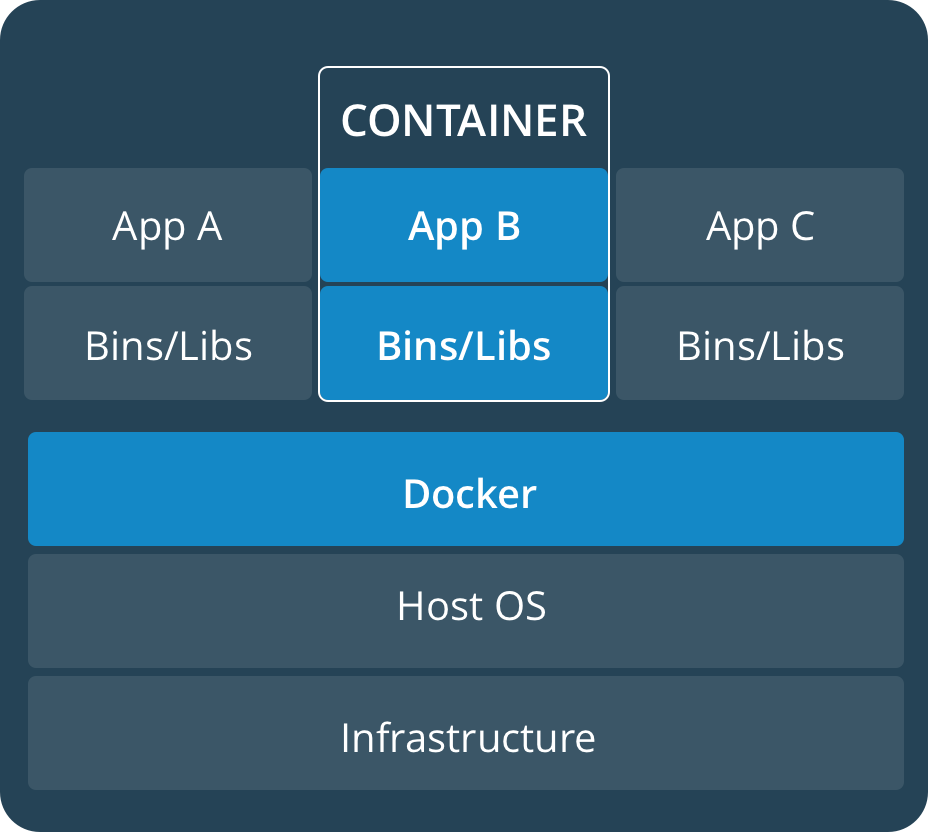
\includegraphics[height=3cm]{img/contenedor.png}~~~
  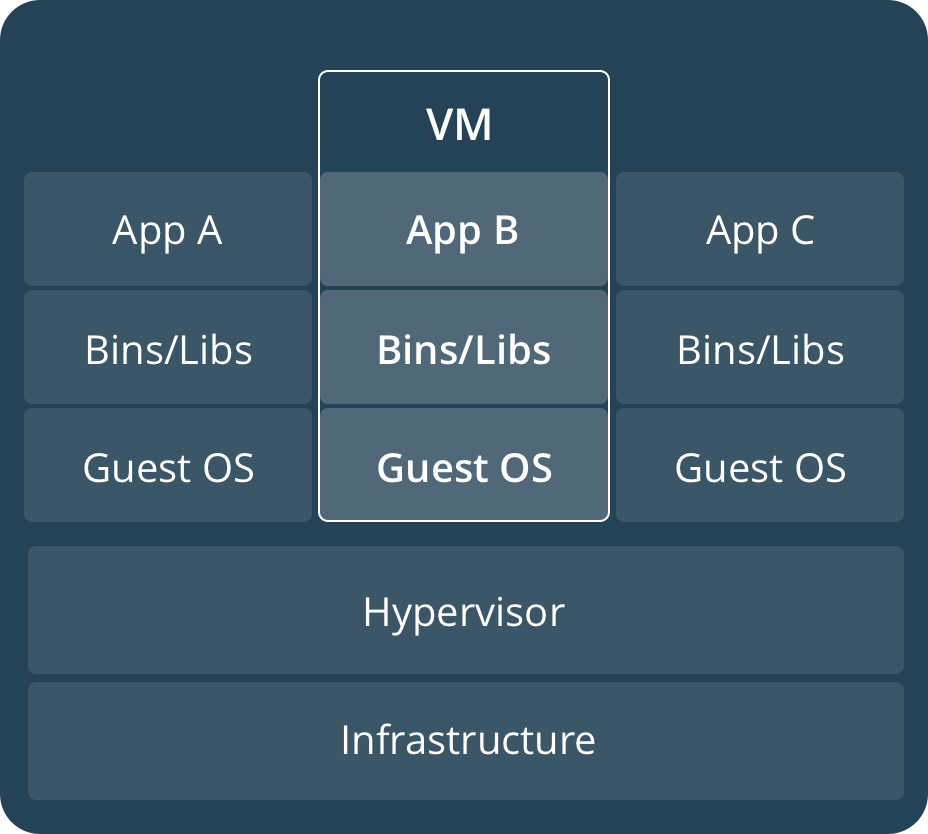
\includegraphics[height=3cm]{img/VM.png}
 \end{center}
\end{frame}

\subsection{Get started}

\begin{frame}[fragile,allowframebreaks]{Docker installation}
\begin{enumerate}
 \item Set up the repository:
\begin{lstlisting}[language=shell]
$ sudo apt-get update # Update the package index
$ sudo apt-get install ca-certificates curl gnupg lsb-release # Install packages to allow apt to use a repository over HTTP
$  curl -fsSL https://download.docker.com/linux/ubuntu/gpg | sudo gpg --dearmor -o /usr/share/keyrings/docker-archive-keyring.gpg  # Add Docker's official GPG key
$ echo "deb [arch=$(dpkg --print-architecture) signed-by=/usr/share/keyrings/docker-archive-keyring.gpg] https://download.docker.com/linux/ubuntu $(lsb_release -cs) stable" | sudo tee /etc/apt/sources.list.d/docker.list > /dev/null # Use the following command to set up the stable repository
\end{lstlisting}
 \framebreak
 \item Install Docker CE:
\begin{lstlisting}[language=shell]
$ sudo apt-get update # Update the package index
$ sudo apt-get install apt-get install docker-ce docker-ce-cli containerd.io # Install the latest version of Docker CE
$ sudo docker run hello-world # Verify that Docker CE is installed correctly by running the hello-world image.
...
Hello from Docker!
This message shows that your installation appears to be working correctly.
...
\end{lstlisting}

 \item Post-installation
  \begin{itemize}
   \item Manage Docker as a non-root user:
\begin{lstlisting}[language=shell]
$ sudo groupadd docker # Create the docker group
$ sudo usermod -aG docker $USER # Add your user to the docker group. Log out and log back in so that your group membership is re-evaluated or run 'newgrp docker' to activate the changes to groups
$ docker run hello-world # Verify that you can run docker commands without sudo
\end{lstlisting}
  \end{itemize}
\end{enumerate}
\end{frame}

% \begin{frame}[fragile]{BusyBox}
%  \begin{itemize}
%   \item Fetch the \textbf{busybox} image from the \textbf{Docker registry}:
% \begin{lstlisting}[language=shell]
% $ docker pull busybox
% \end{lstlisting}
  
%   \item You can use the \texttt{docker images} command to see a list of all images on your system:
% \begin{lstlisting}[language=shell]
% $ docker images
% \end{lstlisting}

%   \item Run a Docker container based on this image:
% \begin{lstlisting}[language=shell]
% $ docker run busybox
% $
% $ docker run busybox echo "hello from busybox"
% hello from busybox
% \end{lstlisting}
  
%   \item \texttt{docker ps} command shows you all containers that are currently running.
% \begin{lstlisting}[language=shell]
% $ docker ps
% CONTAINER ID        IMAGE               COMMAND             CREATED             STATUS              PORTS               NAMES
% $ docker ps -a
% ...
% \end{lstlisting}
%  \end{itemize}
% \end{frame}

\begin{frame}[fragile]{Basic commands}
 \begin{itemize}
  \item List Docker CLI commands:
\begin{lstlisting}[language=shell]
$ docker
$ docker container --help
\end{lstlisting}

  \item Display Docker version and info:
\begin{lstlisting}[language=shell]
$ docker --version
$ docker version
$ docker info
\end{lstlisting}

  \item Execute Docker images:
\begin{lstlisting}[language=shell]
$ docker run hello-world
$ docker run -it <image> sh # -it attaches us to an interactive tty in the container
\end{lstlisting}

  \item List Docker images/networks/containers:
\begin{lstlisting}[language=shell]
$ docker image ls
$ docker network ls
$ docker container ls        # containers running
$ docker container ls --all  # all
$ docker container ls -a -q  # all in quiet mode
$ docker ps
\end{lstlisting}
 \end{itemize}
\end{frame}

\subsection{Define a container}

\begin{frame}[fragile]{Sample application}
 \begin{itemize}
  \item Create a simple Python application using the Flask framework:
\begin{lstlisting}[language=shell]
$ cd /path/to/app
$ pip3 install Flask
$ pip3 freeze | grep Flask >> requirements.txt
$ touch app.py  
\end{lstlisting}

  \item Enter the following code into the \texttt{app.py} file:
\begin{lstlisting}[language=python]
from flask import Flask
app = Flask(__name__)

@app.route('/')
def hello_world():
    return 'Hello, Docker!'
\end{lstlisting}
  
  \item Test the application:
\begin{lstlisting}[language=shell]
$ pwd
/path/to/app
$ python3 -m flask run
\end{lstlisting}
  
  \item Open a browser and navigate to \texttt{http://localhost:5000}. Switch back to the terminal where the server is running and you should see the requests in the server logs.
 \end{itemize}
\end{frame}


\begin{frame}[fragile]{Create a Dockerfile}
\begin{itemize}
  \item \textit{Dockerfile} defines what goes on in the environment inside your container:
\begin{lstlisting}[language=syntax]
FROM python:3.8-slim-buster # Docker images inherit from other base images

WORKDIR /app # default location for all subsequent commands

COPY requirements.txt requirements.txt # copy files into the image
RUN pip3 install -r requirements.txt # execute the command
#RUN pip3 install Flask # Uncomment on Windows and Mac and comment the above lines

COPY . . # Takes all the files located in the current directory and copies them into the image

CMD [ "python3", "-m" , "flask", "run", "--host=0.0.0.0"] # Command to run when the image is executed inside a container
\end{lstlisting}

 \item The Python application directory (\texttt{/path/to/app}) structure would now look like:
\begin{lstlisting}
app
|____ app.py
|____ requirements.txt
|____ Dockerfile
\end{lstlisting}
\end{itemize}
\end{frame}

\begin{frame}[fragile]{Build and run the app}
\begin{itemize}
 \item Build the app:
\begin{lstlisting}[language=shell]
$ pwd
/path/to/app
$ docker build --tag sample-app .
...
$ docker images
...
\end{lstlisting}
 \item Run the app:
\begin{lstlisting}[language=shell]
$ docker run --publish 5000:5000 sample-app
\end{lstlisting}

 \item In a new terminal:
\begin{lstlisting}[language=shell]
$ curl localhost:5000
Hello, Docker!
\end{lstlisting}

 \item Run the app in the background, in detached mode:
\begin{lstlisting}[language=shell]
$ docker run -d -p 5000:5000 sample-app
$ docker ps
$ docker stop CONTAINER_ID
$ docker ps
\end{lstlisting}
\end{itemize}
\end{frame}

\subsection{Rocker}
\begin{frame}[fragile]{Rocker}

 \begin{alertblock}{Rocker}
  Herramienta que permite ejecutar imágenes de Docker con soporte local, por ejemplo soporte de nvidia. Dando la posibilidad de abrir interfaces gráficas en el equipo host. 
  
  \url{https://github.com/osrf/rocker}
 \end{alertblock}

\begin{itemize}
    \item Installation:
\begin{lstlisting}[language=shell]
$ pip install rocker
\end{lstlisting}

    \item Extensions:
    \begin{itemize}
        \item x11 -- Enable the use of X11 inside the container via the host X instance.
        \item nvidia -- Enable NVIDIA graphics cards for rendering
        \item cuda -- Enable NVIDIA CUDA in the container
        \item user -- Create a user inside the container with the same settings as the host and run commands inside the container as that user.
        \item home -- Mount the user's home directory into the container
        \item pulse -- Mount pulse audio into the container
        \item ssh -- Pass through ssh access to the container.
    \end{itemize}
\end{itemize}
    
\end{frame}

\subsection{Docker Hub}
\begin{frame}[fragile]{Docker Hub}
\begin{alertblock}{Docker Hub}
    Repositorio de imágenes docker.
  
  \url{https://hub.docker.com/}
 \end{alertblock}
 
\begin{itemize}
    \item Download an image:
\begin{lstlisting}[language=shell]
$ docker pull <name of the image>
\end{lstlisting}
    
\end{itemize}
    
\end{frame}


%\part{Robot Operating System (ROS)}

\begin{frame}{References}
\begin{columns}[b]
\begin{column}{.32\textwidth}
 \begin{figure}
  
\includegraphics[width=\columnwidth]{./img/ros/ros_org.png}
  \caption{\textbf{ROS wiki}
  
  \url{http://wiki.ros.org/}
  
  The \href{http://wiki.ros.org/}{ROS wiki} is licensed under the \href{http://creativecommons.org/licenses/by/3.0/}{Creative Commons Attribution 3.0}.}
 \end{figure}
\end{column}
\begin{column}{.32\textwidth}
 \begin{figure}
  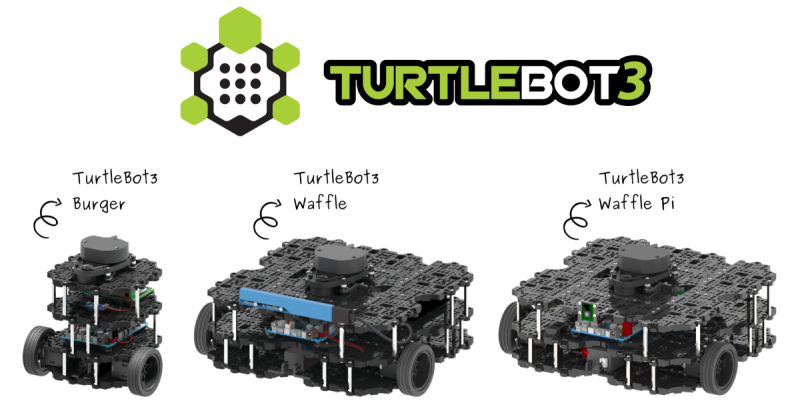
\includegraphics[width=\columnwidth]{./img/ros/turtlebot3.png}
  \caption{\textbf{Robotis e-Manual}
  
  \url{http://emanual.robotis.com/docs/en/platform/turtlebot3/overview/}}
 \end{figure}
\end{column}
\begin{column}{.32\textwidth}
 \begin{figure}
  
\includegraphics[width=.5\columnwidth]{./img/ros/masteringbook.jpg}
  \caption{Joseph, L., \& Cacace, J. (2018). \href{https://www.amazon.es/Mastering-Robotics-Programming-Lentin-Joseph/dp/1783551798}{Mastering ROS for Robotics Programming: Design, build, and simulate complex robots using the Robot Operating System}. Packt Publishing Ltd.}
 \end{figure}
\end{column}
\end{columns}
\end{frame}


% \section{Parts of a robot}
% \begin{frame}{Parts of a robot}
% \begin{figure}
%     \centering
%     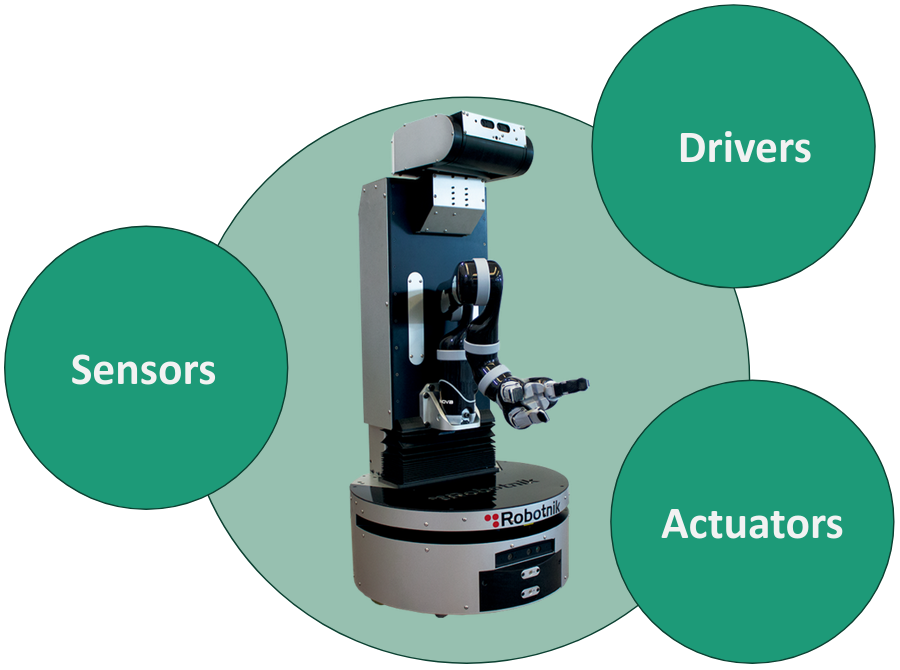
\includegraphics[scale=0.3]{img/ros/partes_robot.png}
% \end{figure}
% \end{frame}

\section{ROS Concepts}
%TODO intro ROS (ROBOT17) y completar filesystem level, community level

\begin{frame}[allowframebreaks]{ROS overview}
 \begin{block}{Robot Operating System (ROS)}
 ROS is basically a set of libraries for robotics similar to operating system services, providing hardware abstraction for sensors and actuators, low-level device control, and inter-process communication. 
 \end{block}
 
 \begin{itemize}
  \item The ROS project was started in 2007, 
  \item with the name \textit{Switchyard}, by Morgan Quigley (\url{wiki.osrfoundation.org/morgan}), 
  \item as part of the Stanford STAIR robot project. 
  %\item The main development of ROS happened at Willow Garage (\url{www.willowgarage.com}).
 \end{itemize}
 


  \framebreak
 \begin{figure}
  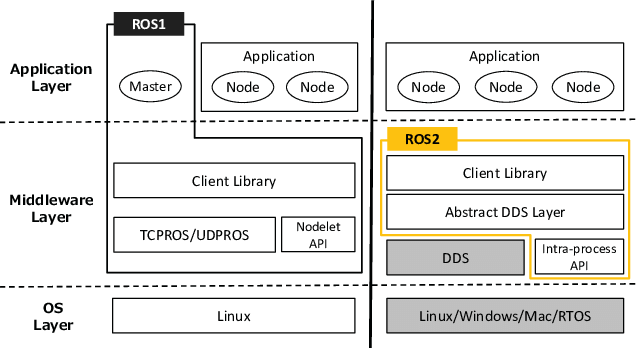
\includegraphics[width=.7\textwidth]{./img/ros/ROS1-ROS2-architecture.png}
 \end{figure}

 

  \framebreak
 \textbf{Why ROS?}
 \begin{itemize}
			\item High-end capabilities: ROS comes with ready-to-use capabilities.
			\item Myriad of tools: ROS is packed with tons of tools for debugging, visualizing, and
			performing a simulation.
			\item Support for high-end sensors and actuators: ROS is packed with device drivers
			and interface packages of various sensors and actuators in robotics.
			\item Inter-platform operability: The ROS message-passing middleware allows
			communication between different nodes. These nodes can be programmed in any
			language that has ROS client libraries.
			\item Modularity: One of the issues that can occur in most of the standalone robotic
			applications is that if any of the threads of main code crash, the entire robot
			application can stop.
			\item Concurrent resource handling: Handling a hardware resource via more than two
			processes is always a headache.
			\item Active community: When we choose a library or software framework,  one of the main factors that needs to be checked before using it is its software support and developer community.
 \end{itemize}
 
 \framebreak
 
 \textbf{Why not?}
		\begin{itemize}
			\item Difficulty in learning:  ROS   has a steep learning curve and developers should become familiar with many new concepts to get the expected benefits.
			\item Difficulties in starting with simulation: The main simulator in ROS is Gazebo.
			Even though Gazebo works well (it requires medium-high computer specs), to get started with Gazebo is not an easy task.
			\item Difficulties in robot modeling: The robot modeling in ROS is performed using
			URDF, which is an XML-based robot description. 
			\item Potential limitations: Current limitations in fields as real time or cibersegurity. 
			\item ROS in commercial robot products:  ROS on a commercial
			product. It needs a lot of things to be taken care of before to stay in public spaces and  long-term scenarios.
		\end{itemize}
  
 \framebreak
 
 \begin{block}{ROS framework} 
 ROS framework is a message-passing distributed system. 
 \begin{itemize}
  \item Computation takes place in processes named \textbf{nodes} 
  \item which can receive and send \textbf{messages} 
  \item throught information buffers called \textbf{topics}. 
 \end{itemize}  
 
 \end{block}
 
 \begin{figure}
  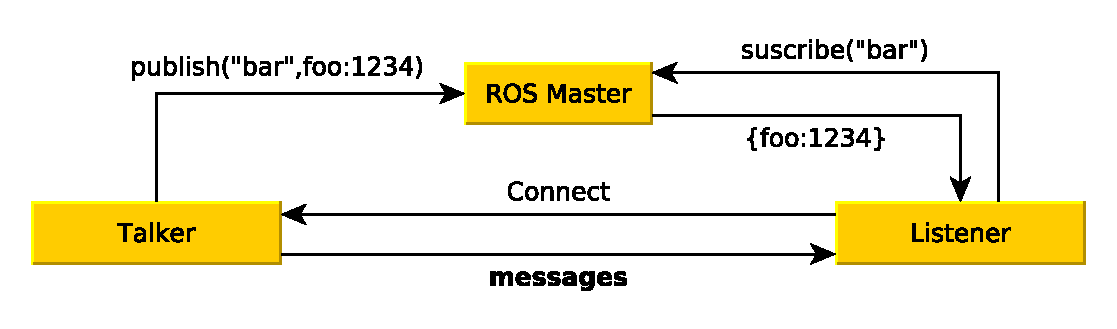
\includegraphics[width=.8\textwidth]{./img/ros/ros.pdf}
 \end{figure}
\end{frame}

\begin{frame}[allowframebreaks]{ROS Computation Graph level}
The \textbf{Computation Graph} is the peer-to-peer network of ROS processes that are processing data together. 

 \begin{figure}
	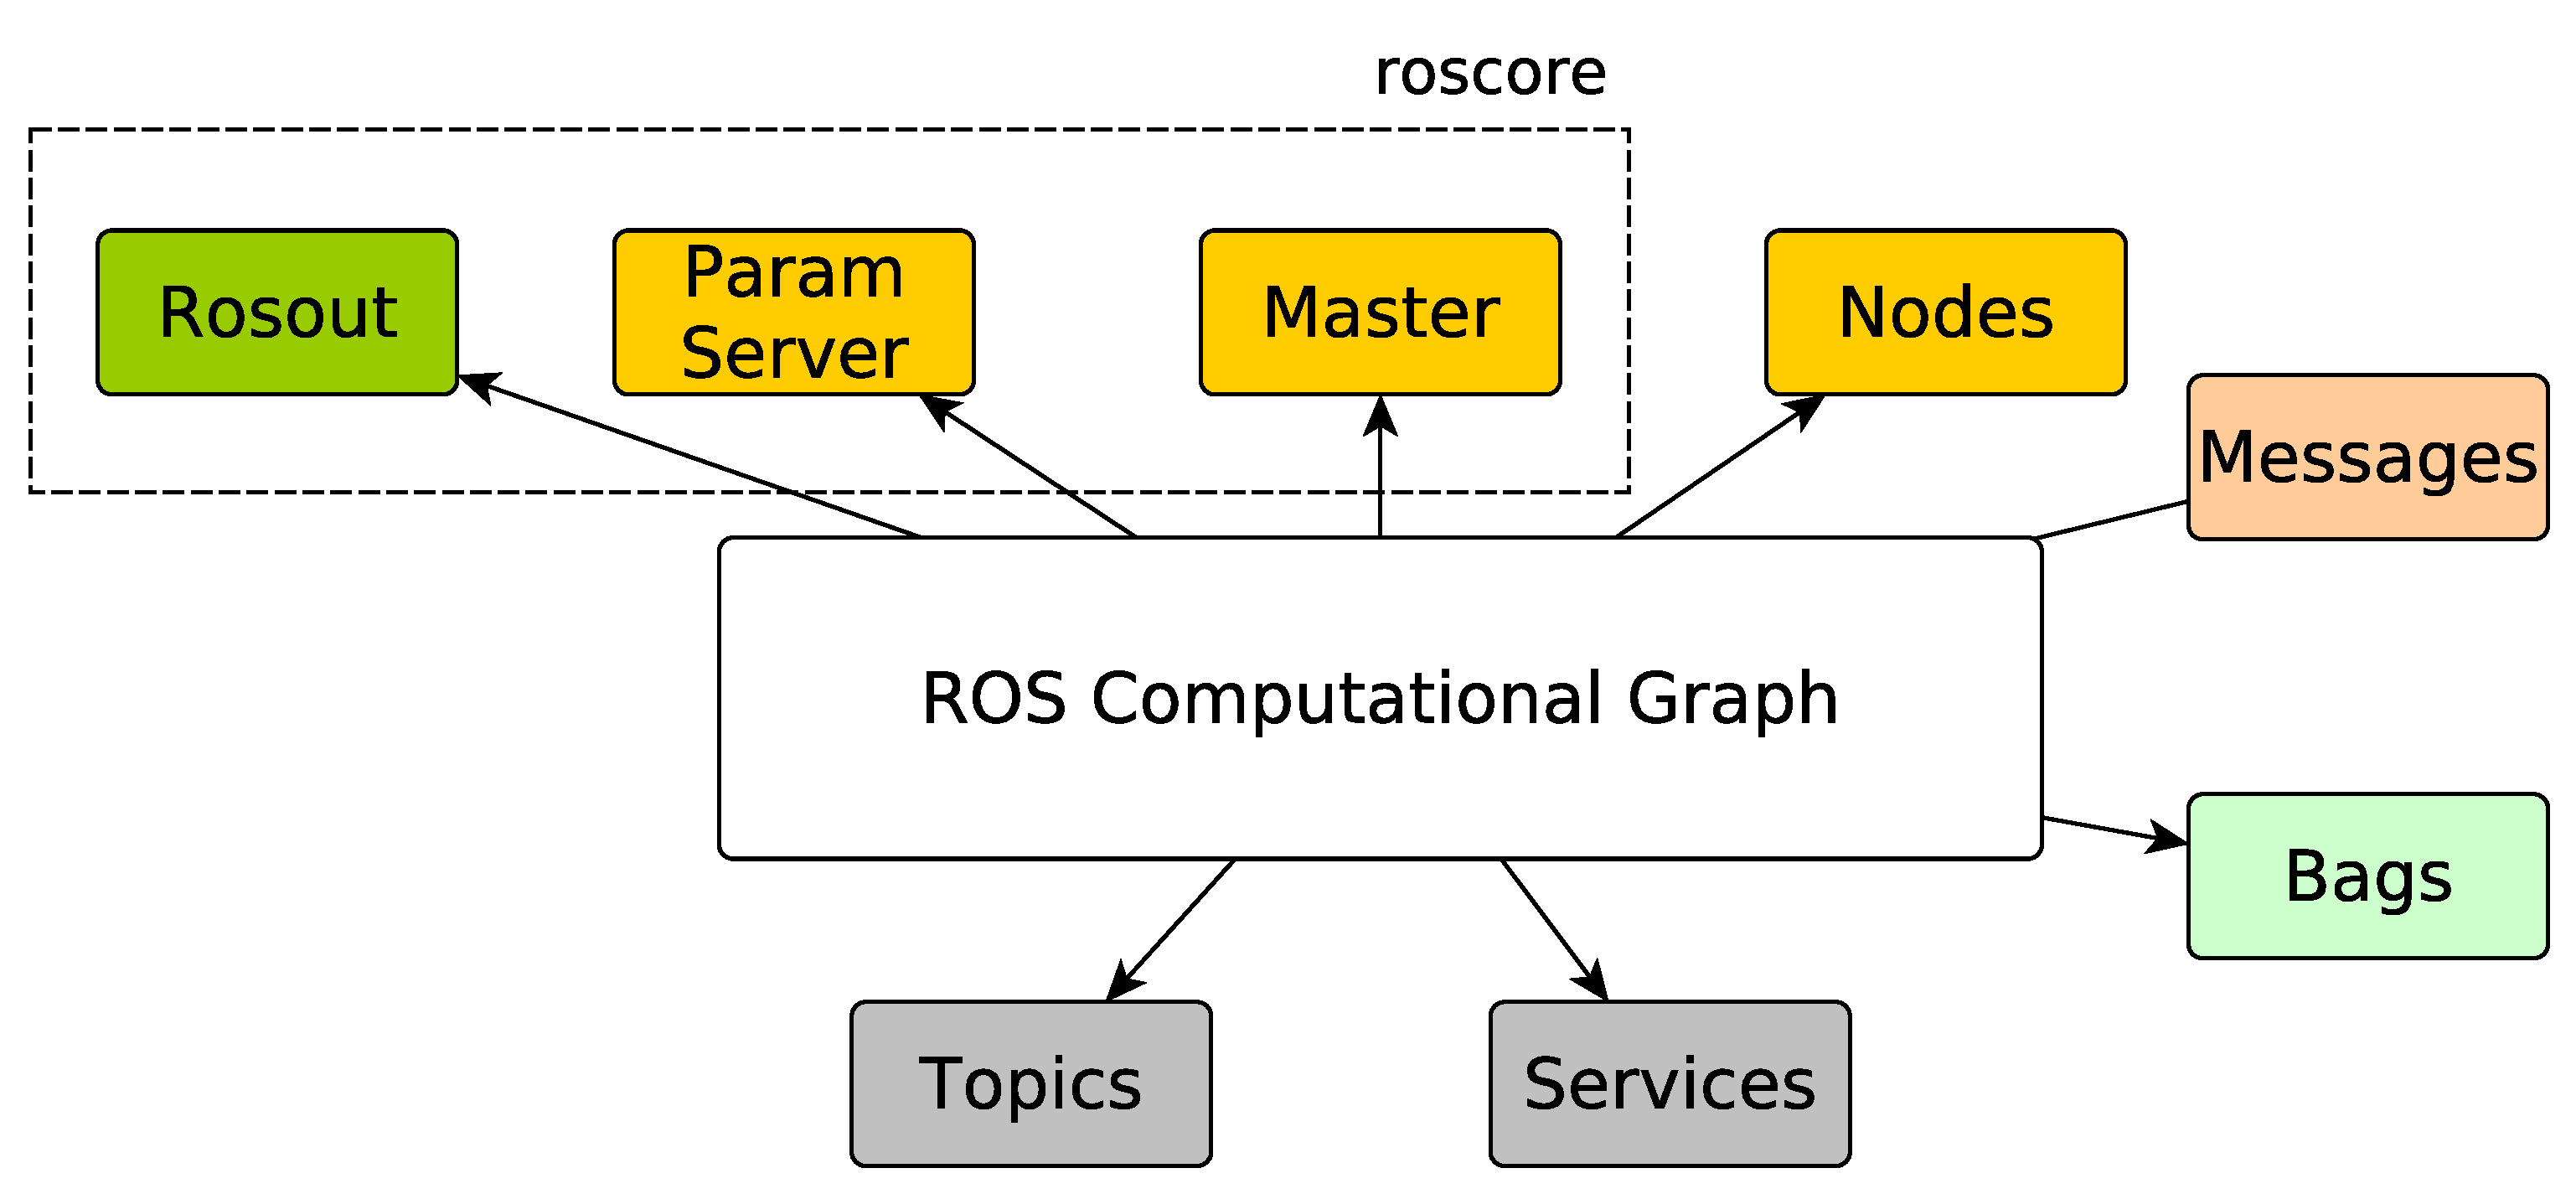
\includegraphics[width=.6\textwidth]{./img/ros/RosGraph.pdf}
 \end{figure}
 
Basic \textbf{Computation Graph concepts} of ROS:

 \begin{description}[leftmargin=10.1cm]
  \item[Nodes] A node is an executable that uses ROS to communicate with other nodes.
  \item[Messages] ROS data type used when subscribing or publishing to a topic.
  \item[Topics] Nodes can publish messages to a topic as well as subscribe to a topic to receive messages.
  \item[Master] Name service for ROS (i.e. helps nodes find each other).
  \item[rosout] ROS equivalent of stdout/stderr.
  \item[Parameter Server] Allows data to be stored by key in a central location.
  \item[roscore] Master + Rosout + Parameter Server.
  \item[Services] Request/reply interaction is done via services, which are defined by a pair of message structures: one for the request and one for the reply. A providing node offers a service under a name and a client uses the service by sending the request message and awaiting the reply.
  \item[Bags] Bags are a format for saving and playing back ROS message data. Bags are an important mechanism for storing data, such as sensor data, that can be difficult to collect but is necessary for developing and testing algorithms.
 \end{description}
 
\end{frame}

\begin{frame}{Example}
\begin{figure}
    \centering
    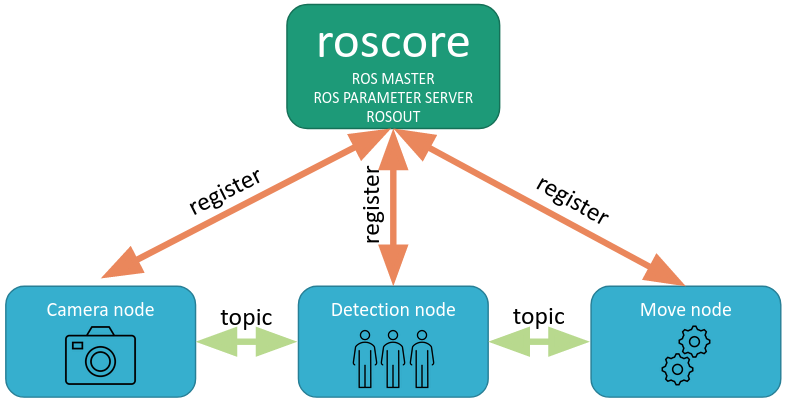
\includegraphics[scale=0.4]{img/ros/nodos_topics.png}
\end{figure}

\end{frame}

\section{ROS basics}

\subsection{Installing and configuring your ROS environment}

\begin{frame}[fragile, allowframebreaks]{Ubuntu install of ROS noetic}
ROS noetic \textbf{ONLY} supports FocalFossa (Ubuntu 20.04) and Buster (Debian 10) for debian packages. 
\begin{enumerate}
 \item Setup your computer to \textbf{accept software from packages.ros.org}:
\begin{lstlisting}[language=shell]
$ sudo sh -c 'echo "deb http://packages.ros.org/ros/ubuntu $(lsb_release -sc) main" > /etc/apt/sources.list.d/ros-latest.list'
\end{lstlisting}
 \item Set up your \textbf{keys}:
\begin{lstlisting}[language=shell]
$ sudo apt install curl # if you haven't already installed curl
$ curl -s https://raw.githubusercontent.com/ros/rosdistro/master/ros.asc | sudo apt-key add -
\end{lstlisting}
 \item \textbf{Installation}:
\begin{lstlisting}[language=shell]
$ sudo apt-get update
$ sudo apt install ros-noetic-desktop-full
\end{lstlisting}
 \item \textbf{Initialize rosdep}.
 
 \vspace{.1cm}
 Before you can use ROS, you will need to initialize \textit{rosdep}. rosdep enables you to easily install system dependencies for source you want to compile and is required to run some core components in ROS. 
\begin{lstlisting}[language=shell]
$ sudo apt install python3-rosdep
$ sudo rosdep init
$ rosdep update
\end{lstlisting}

 \item \textbf{Environment setup}.

 \vspace{.1cm}
 It's convenient if the ROS environment variables are automatically added to your bash session every time a new shell is launched.
\begin{lstlisting}[language=shell]
$ echo "source /opt/ros/noetic/setup.bash" >> ~/.bashrc
$ source ~/.bashrc
\end{lstlisting}

 \framebreak
 
 \item \textbf{Dependencies for building packages}.

 \vspace{.1cm}
 To install \textit{rosinstall} and other dependencies for building ROS packages, run: 
\begin{lstlisting}[language=shell]
sudo apt install python3-rosdep python3-rosinstall python3-rosinstall-generator python3-wstool build-essential
\end{lstlisting}
\end{enumerate}
\end{frame}

\begin{frame}[fragile, allowframebreaks]{Setting up docker image}

\begin{enumerate}
    \item Download the image from Docker Hub
\begin{lstlisting}[language=shell]
$ docker pull osrf/ros:noetic-desktop-full
\end{lstlisting}
    \item Launch the container using Rocker
\begin{lstlisting}[language=shell]
$ rocker --nvidia --x11 --network host --name ros-noetic  --volume <path_to_shared_folder>:/root/catkin_ws -- docker.io/osrf/ros:noetic-desktop-full
\end{lstlisting}
\textcolor{blue}{- -nvidia option only if the computer has a graphic card}\\
\textcolor{blue}{- -volume only if you want to share a folder between the host and the container.\textit{Important for save changes that you do inside the container}}
    \item To open a new terminal inside the container:
\begin{lstlisting}[language=shell]
$ docker exec -it ros-noetic /bin/bash 
\end{lstlisting}    
\newpage
\item To source the ROS environment:
\begin{lstlisting}[language=shell]
$ source /opt/ros/noetic/setup.bash
\end{lstlisting}  
\item To source the software installed in the workspace (\textit{necessary have executed before a catkin\_make}):
\begin{lstlisting}[language=shell]
$ source /root/catkin_ws/devel/setup.bash
\end{lstlisting}  
    
\end{enumerate}
\end{frame}

\begin{frame}[fragile]{Create a ROS Workspace}
Let's create and build a catkin workspace: 

\begin{lstlisting}[language=shell]
$ mkdir -p ~/catkin_ws/src
$ cd ~/catkin_ws/
$ catkin_make
\end{lstlisting}

The catkin\_make command is a convenience tool for working with catkin workspaces. Running it the first time in your workspace, it will create a \texttt{CMakeLists.txt} link in your `src' folder. 

\vspace{.1cm}
Additionally, if you look in your current directory you should now have a `build' and `devel' folder. Inside the 'devel' folder you can see that there are now several setup.*sh files. 

\vspace{.1cm}
Sourcing any of these files will overlay this workspace on top of your environment. Before continuing source your new setup.*sh file: 

\begin{lstlisting}[language=shell]
$ source devel/setup.bash
\end{lstlisting}

To make sure your workspace is properly overlayed by the setup script, make sure ROS\_PACKAGE\_PATH environment variable includes the directory you're in. 

\begin{lstlisting}[language=shell]
$ echo $ROS_PACKAGE_PATH
/home/youruser/catkin_ws/src:/opt/ros/noetic/share
\end{lstlisting}
\end{frame}

\subsection{Navigating the ROS Filesystem}

\begin{frame}[fragile,allowframebreaks]{Filesystem concepts}
 \begin{description}[leftmargin=10.1cm]
  \item[Packages] Packages are the software organization unit of ROS code. Each package can contain libraries, executables, scripts, or other artifacts. 
  \item[Manifests] (package.xml) A manifest is a description of a package. It serves to define dependencies between packages and to capture meta information about the package like version, maintainer, license, etc...
  \item[Metapackage] Metapackages are specialized Packages which only serve to represent a group of related other packages.
 \end{description}
 
  \begin{figure}
 	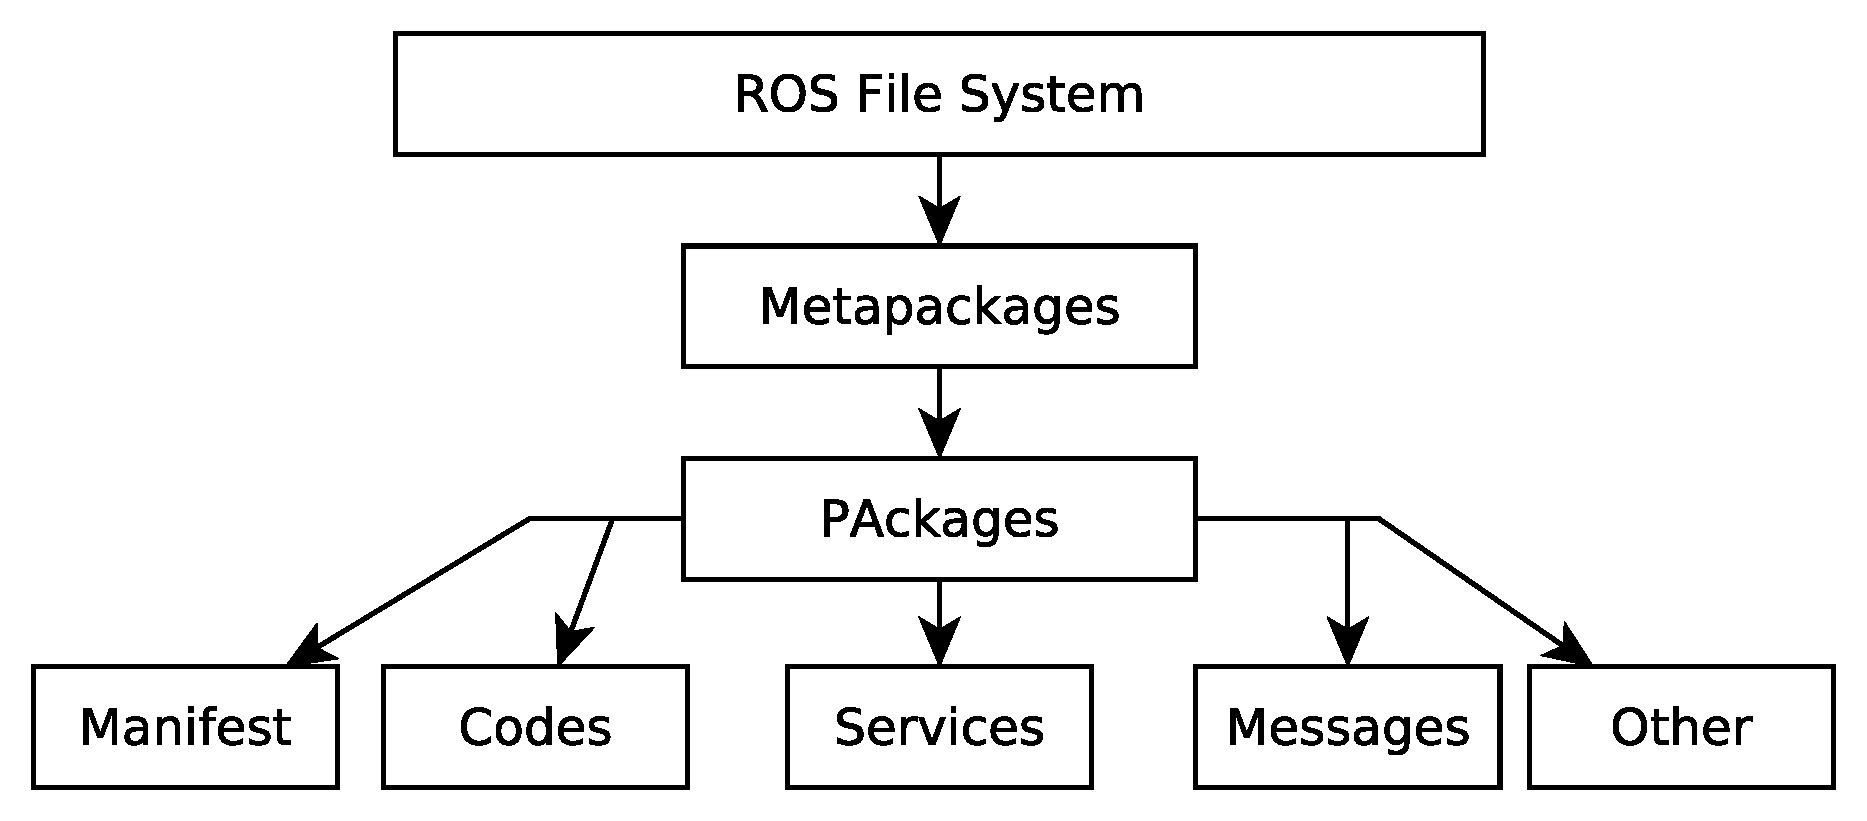
\includegraphics[width=.5\textwidth]{./img/ros/RosFilesystem.pdf}
 \end{figure}%TODO citar packt 
 
 \framebreak
 
 \begin{alertblock}{Prerequisites}
  We will inspect a package in ros-tutorials, please install it using:
\begin{lstlisting}[language=shell]
$ sudo apt-get install ros-<distro>-ros-tutorials
\end{lstlisting}
  Replace `$<$distro$>$' (including the `$<>$') with the name of your ROS distribution (e.g. indigo, kinetic, lunar etc.). 
 \end{alertblock}
\end{frame}

\begin{frame}[fragile,allowframebreaks]{Filesystem tools}
 \begin{itemize}  
  \item \textbf{rospack}: allows to get information about packages.
\begin{lstlisting}[language=syntax]
rospack find [package_name]
\end{lstlisting}
\begin{lstlisting}[language=shell]
$ rospack find roscpp
/opt/ros/noetic/share/roscpp
\end{lstlisting}

  \item \textbf{roscd}: allows to change directory (cd) directly to a package or a stack. 
\begin{lstlisting}[language=syntax]
roscd [locationname[/subdir]]
\end{lstlisting}
\begin{lstlisting}[language=shell]
$ roscd roscpp
$ pwd
/opt/ros/noetic/share/roscpp
\end{lstlisting}
\begin{lstlisting}[language=shell]
$ roscd roscpp/cmake
$ pwd
/opt/ros/noetic/share/roscpp/cmake
\end{lstlisting}

  \item \textbf{roscd log} will take you to the folder where ROS stores log files. Note that if you have not run any ROS programs yet, this will yield an error saying that it does not yet exist. 
\begin{lstlisting}[language=shell]
$ roscd log
$ pwd
/home/youruser/.ros/log
\end{lstlisting}

  \item \textbf{rosls}: allows to ls directly in a package by name rather than by absolute path. 
\begin{lstlisting}[language=syntax]
rosls [locationname[/subdir]]
\end{lstlisting}
\begin{lstlisting}[language=shell]
$ rosls roscpp_tutorials
cmake launch package.xml  srv
\end{lstlisting}
 \end{itemize}

 \begin{alertblock}{TAB completion}
  Some ROS tools support TAB completion.  
 \end{alertblock}
\end{frame}

\subsection{Creating and building ROS Packages}

\begin{frame}[fragile]{What makes up a catkin Package?}
For a package to be considered a catkin package it must meet a few requirements: 
\begin{itemize}
 \item The package must contain a catkin compliant package.xml file. 
 \item The package must contain a CMakeLists.txt which uses catkin. 
 \item Each package must have its own folder 
\end{itemize}

The recommended method of working with catkin packages is using a catkin workspace, but you can also build catkin packages standalone. A trivial workspace might look like this: 
\begin{lstlisting}[language=syntax]
workspace_folder/        -- WORKSPACE
  src/                   -- SOURCE SPACE
    CMakeLists.txt       -- 'Toplevel' CMake file, provided by catkin
    package_1/
      CMakeLists.txt     -- CMakeLists.txt file for package_1
      package.xml        -- Package manifest for package_1
    ...
    package_n/
      CMakeLists.txt     -- CMakeLists.txt file for package_n
      package.xml        -- Package manifest for package_n
\end{lstlisting}
\end{frame}

\begin{frame}[fragile]{Creating a catkin Package}
The \textbf{catkin\_create\_pkg} script allows to create new packages. It requires that you give it a package name and optionally a list of dependencies on which that package depends: 

\begin{lstlisting}[language=syntax]
catkin_create_pkg <package_name> [depend1] [depend2] [depend3]
\end{lstlisting}

First change to the source space directory of the catkin workspace.

\begin{lstlisting}[language=shell]
$ cd ~/catkin_ws/src
\end{lstlisting}

Now use the catkin\_create\_pkg script to create a new package called `my\_first\_package' which depends on std\_msgs, roscpp, and rospy: 

\begin{lstlisting}[language=shell]
$ catkin_create_pkg my_first_package std_msgs rospy roscpp
\end{lstlisting}
\end{frame}

\begin{frame}[fragile]{Building a catkin workspace and sourcing the setup file}
\textbf{catkin\_make} allows to build the packages in the catkin workspace: 

\begin{lstlisting}[language=shell]
$ cd ~/catkin_ws
$ catkin_make
\end{lstlisting}

After the workspace has been built it has created a similar structure in the devel subfolder as you usually find under /opt/ros/\$ROS\_DISTRO.

\vspace{.1cm}
To add the workspace to your ROS environment you need to source the generated setup file: 

\begin{lstlisting}[language=shell]
$ source ~/catkin_ws/devel/setup.bash
\end{lstlisting}

It's convenient if the ROS environment variables are automatically added to your bash session every time a new shell is launched.
\begin{lstlisting}[language=shell]
$ echo "source /home/youruser/catkin_ws/devel/setup.bash" >> ~/.bashrc
$ source ~/.bashrc
\end{lstlisting}
\end{frame}

\begin{frame}[fragile,allowframebreaks]{Package dependencies}
 \begin{itemize}
  \item \textbf{First-order dependencies}
  
  \vspace{.1cm}
  When using catkin\_create\_pkg earlier, a few package dependencies were provided. These first-order dependencies can now be reviewed with the rospack tool. 
\begin{lstlisting}[language=shell]
$ rospack depends1 my_first_package
roscpp
rospy
std_msgs
\end{lstlisting}
  These dependencies for a package are stored in the package.xml file: 
\begin{lstlisting}[language=shell]
$ roscd my_first_package && cat package.xml
<package format="2">
...
  <buildtool_depend>catkin</buildtool_depend>
  <build_depend>roscpp</build_depend>
  <build_depend>rospy</build_depend>
  <build_depend>std_msgs</build_depend>
...
</package>
\end{lstlisting}  
  \item \textbf{Indirect dependencies}
  
  \vspace{.1cm}
  A package can have quite a few indirect dependencies. Luckily rospack can recursively determine all nested dependencies. 
\begin{lstlisting}[language=shell]
$ rospack depends my_first_package
cpp_common
rostime
roscpp_traits
roscpp_serialization
catkin
genmsg
genpy
message_runtime
gencpp
geneus
gennodejs
...
\end{lstlisting}
 \end{itemize}
\end{frame}

\begin{frame}[fragile]{Customizing the package.xml}
\begin{lstlisting}[language=xml]
<?xml version="1.0"?>
<package format="2">
  <name>my_first_package</name>
  <version>0.1.0</version>
  <description>The my_first_package package</description>

  <maintainer email="you@yourdomain.tld">Your Name</maintainer>
  <license>BSD</license>
  <url type="website">http://wiki.ros.org/beginner_tutorials</url>
  <author email="you@yourdomain.tld">Jane Doe</author>

  <buildtool_depend>catkin</buildtool_depend>

  <build_depend>roscpp</build_depend>
  <build_depend>rospy</build_depend>
  <build_depend>std_msgs</build_depend>

  <exec_depend>roscpp</exec_depend>
  <exec_depend>rospy</exec_depend>
  <exec_depend>std_msgs</exec_depend>
</package>
\end{lstlisting}
\end{frame}

\subsection{Understanding ROS Nodes}

\begin{frame}{Nodes}
 \begin{itemize}
  \item A node really isn't much more than an executable file within a ROS package. 
  \item Nodes can publish or subscribe to a Topic. 
  \item Nodes can also provide or use a Service.
  \item ROS nodes use a \textbf{ROS client library} to communicate with other nodes. 
  \item ROS client libraries allow nodes written in different programming languages to communicate: 
   \begin{itemize}
    \item rospy = python client library 
    \item roscpp = c++ client library 
   \end{itemize}
 \end{itemize}
\end{frame}

\begin{frame}[fragile]{roscore}
\textbf{roscore} is the first thing you should run when using ROS. 
\begin{lstlisting}[language=shell]
$ roscore
...
SUMMARY
======

PARAMETERS
 * /rosversion
 * /rosdistro

NODES

auto-starting new master
process[master]: started with pid [13054]
ROS_MASTER_URI=http://machine_name:11311/

setting /run_id to 9cf88ce4-b14d-11df-8a75-00251148e8cf
process[rosout-1]: started with pid [13067]
started core service [/rosout]
\end{lstlisting}
\end{frame}

\begin{frame}[fragile,allowframebreaks]{Using rosnode}
\textbf{rosnode} displays information about the ROS nodes that are currently running. The rosnode list command lists these active nodes: 
\begin{lstlisting}[language=shell]
$ rosnode list
/rosout
\end{lstlisting}
This showed us that there is only one node running: rosout. This is always running as it collects and logs nodes' debugging output. 

\vspace{.1cm}
The \textbf{rosnode info} command returns information about a specific node. 
\begin{lstlisting}[language=shell]
$ rosnode info /rosout
------------------------------------------------------------------------
Node [/rosout]
Publications:
 * /rosout_agg [rosgraph_msgs/Log]

Subscriptions:
 * /rosout [unknown type]

Services:
 * /rosout/get_loggers
 * /rosout/set_logger_level

contacting node http://machine_name:54614/ ...
Pid: 5092
\end{lstlisting}

\begin{alertblock}{Note}
When opening a new terminal your environment is reset and your ~/.bashrc file is sourced. If you have trouble running commands like rosnode then you might need to add some environment setup files to your $\sim$/.bashrc or manually re-source them. 
\end{alertblock}
\end{frame}

\begin{frame}[fragile,allowframebreaks]{Using rosrun}
\textbf{rosrun} allows you to use the package name to directly run a node within a package (without having to know the package path). 
\begin{lstlisting}[language=syntax]
rosrun [package_name] [node_name]
\end{lstlisting}
e.g.:
\begin{lstlisting}[language=shell]
$ rosrun turtlesim turtlesim_node
\end{lstlisting}
You will see the turtlesim window. Now, in a new terminal:
\begin{lstlisting}[language=shell]
$ rosnode list
/rosout
/turtlesim
\end{lstlisting}
One powerful feature of ROS is that you can reassign Names from the command-line. Close the turtlesim window to stop the node (or go back to the rosrun turtlesim terminal and use ctrl-C). Now let's re-run it, but this time use a Remapping Argument to change the node's name: 
\begin{lstlisting}[language=shell]
$ rosrun turtlesim turtlesim_node __name:=my_turtle
\end{lstlisting}
Now, if we go back and use rosnode list:
\begin{lstlisting}[language=shell]
$ rosnode list
/my_turtle
/rosout
\end{lstlisting}
Let's use another rosnode command, ping, to test that it's up: 
\begin{lstlisting}[language=shell]
$ rosnode ping my_turtle
rosnode: node is [/my_turtle]
pinging /my_turtle with a timeout of 3.0s
xmlrpc reply from http://aqy:42235/     time=1.152992ms
xmlrpc reply from http://aqy:42235/     time=1.120090ms
xmlrpc reply from http://aqy:42235/     time=1.700878ms
xmlrpc reply from http://aqy:42235/     time=1.127958ms
\end{lstlisting}
\end{frame}

\subsection{Understanding ROS Topics}

\begin{frame}[fragile]{Turtlebot teleoperation}
Please run in a new terminal:
\begin{lstlisting}[language=shell]
$ rosrun turtlesim turtlesim_node
\end{lstlisting}

We'll also need something to drive the turtle around with. Please run in a new terminal:
\begin{lstlisting}[language=shell]
$ rosrun turtlesim turtle_teleop_key
[ INFO] 1254264546.878445000: Started node [/teleop_turtle], pid [5528], bound on [aqy], xmlrpc port [43918], tcpros port [55936], logging to [~/ros/ros/log/teleop_turtle_5528.log], using [real] time
Reading from keyboard
---------------------------
Use arrow keys to move the turtle.
\end{lstlisting}
Now you can use the arrow keys of the keyboard to drive the turtle around. If you can not drive the turtle select the terminal window of the turtle\_teleop\_key to make sure that the keys that you type are recorded.

\vspace{.1cm}
The turtlesim\_node and the turtle\_teleop\_key node are communicating with each other over a \textbf{ROS Topic}. turtle\_teleop\_key is publishing the key strokes on a topic, while turtlesim subscribes to the same topic to receive the key strokes.
\end{frame}

\begin{frame}[fragile]{rqt\_graph}
\textbf{rqt\_graph} creates a dynamic graph of what's going on in the system. rqt\_graph is part of the rqt package. Unless you already have it installed, run:
\begin{lstlisting}[language=shell]
$ sudo apt-get install ros-<distro>-rqt
$ sudo apt-get install ros-<distro>-rqt-common-plugins
\end{lstlisting}
replacing $<$distro$>$ with the name of your ROS distribution (e.g. indigo, jade, kinetic, lunar ...). Now, in a new terminal:
\begin{lstlisting}[language=shell]
$ rosrun rqt_graph rqt_graph
\end{lstlisting}
You will see something similar to:
\begin{figure}
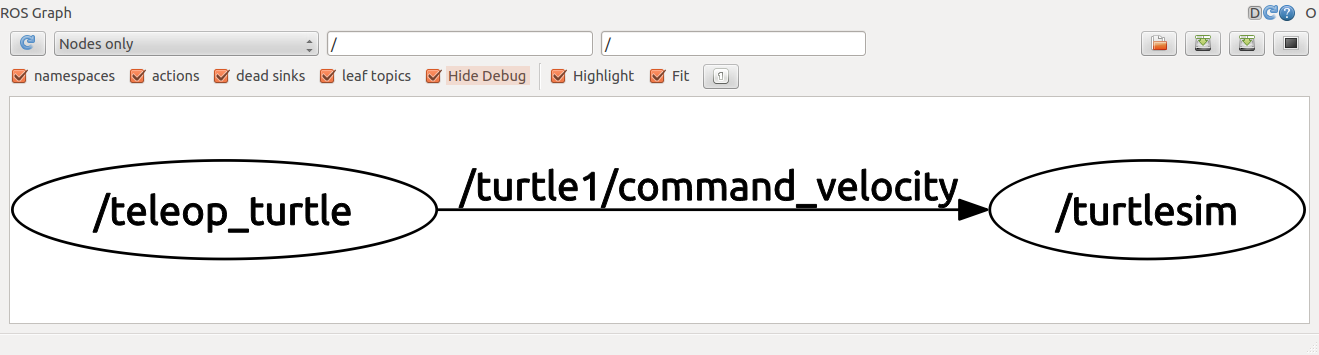
\includegraphics[width=.85\textwidth]{./img/ros/rqt_graph_1.png}
\end{figure}
\end{frame}

\begin{frame}[fragile,allowframebreaks]{ROS messages}
Communication on topics happens by sending ROS \textbf{messages} between nodes. The publisher and subscriber must send and receive the same \textbf{type} of message. The type of the message sent on a topic can be determined using \textbf{rostopic type}.

\begin{lstlisting}[language=syntax]
rostopic type [topic]
\end{lstlisting}

\begin{lstlisting}[language=shell]
$ rostopic type /turtle1/cmd_vel
You should get:
geometry_msgs/Twist
\end{lstlisting}

We can look at the details of the message using \textbf{rosmsg}:

\begin{lstlisting}[language=shell]
$ rosmsg show geometry_msgs/Twist
geometry_msgs/Vector3 linear
  float64 x
  float64 y
  float64 z
geometry_msgs/Vector3 angular
  float64 x
  float64 y
  float64 z
\end{lstlisting}

\framebreak

The message definition can consist of two types: \textbf{fields} and \textbf{constants}. 
\begin{itemize}
		\item  The field type is the data type of the transmitting message. 
		\item The constants define a constant value in the message file.
\end{itemize}

\vspace{.3cm}
Other kinds of messages:
\begin{itemize}
	\item \textbf{Specific}: cover a particular application necessity, such as
	exchanging common geometrical ( geometry\_msgs ) or sensor ( sensor\_msgs ) information.
	\item \textbf{Headers}: Headers can carry information,
	such as time, frame of reference or frame\_id, and sequence number. It is mainly used to send data such as robot joint transforms (TF).
\end{itemize}

\framebreak

	\begin{figure}
		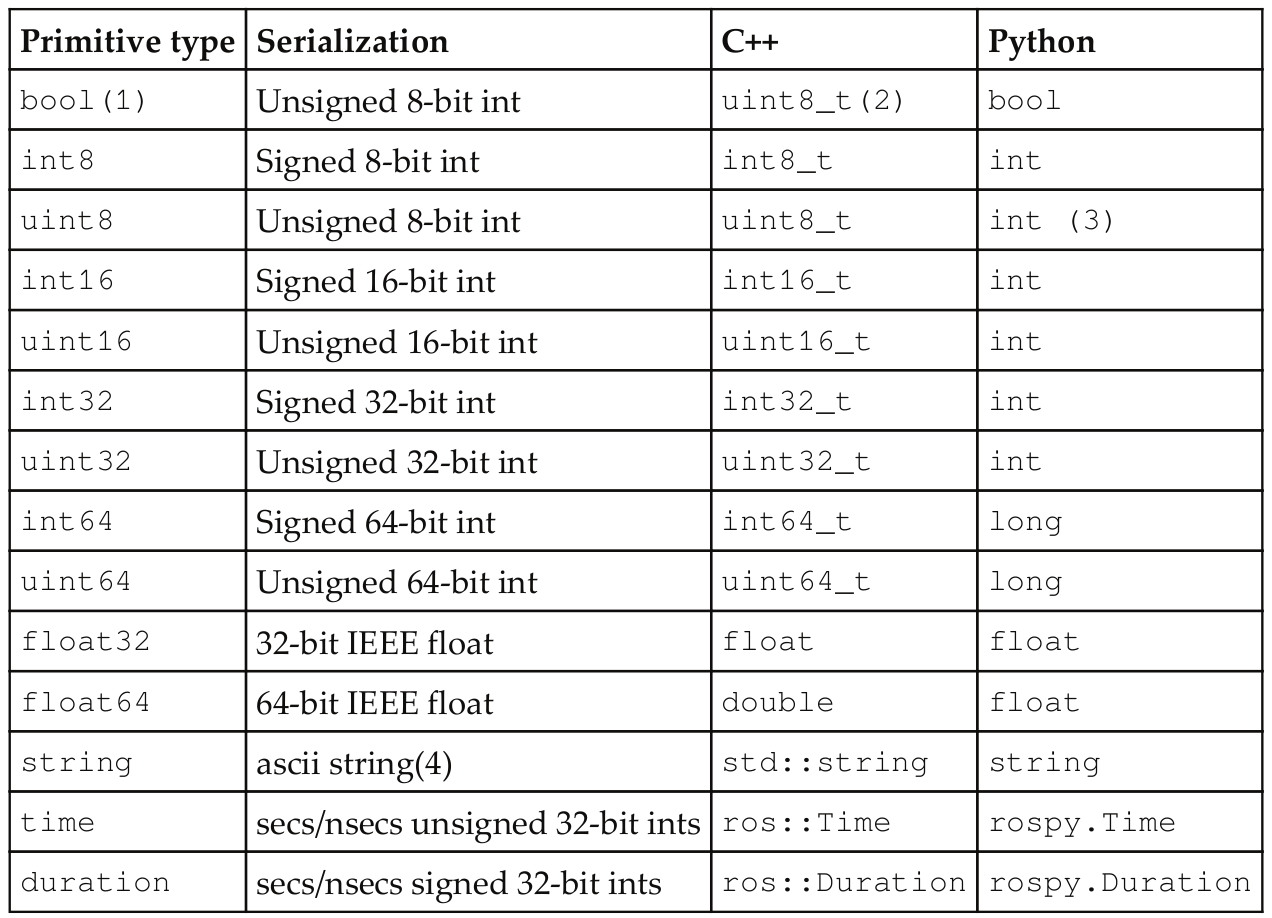
\includegraphics[width=.65\textwidth]{./img/ros/MessageType.png}
	\end{figure}

\end{frame}

\begin{frame}[fragile]{Using rostopic}
The \textbf{rostopic} tool allows you to get information about ROS topics. 

\vspace{.1cm}
You can use the help option to get the available sub-commands for rostopic:
\begin{lstlisting}[language=shell]
$ rostopic -h
rostopic bw     display bandwidth used by topic
rostopic echo   print messages to screen
rostopic hz     display publishing rate of topic    
rostopic list   print information about active topics
rostopic pub    publish data to topic
rostopic type   print topic type
\end{lstlisting}
\end{frame}

\begin{frame}[fragile]{rostopic echo}
\textbf{rostopic echo} shows the data published on a topic.
\begin{lstlisting}[language=syntax]
rostopic echo [topic]
\end{lstlisting}
e.g.:
\begin{lstlisting}[language=shell]
$ rostopic echo /turtle1/cmd_vel
\end{lstlisting}
You probably won't see anything happen because no data is being published on the topic. Let's make turtle\_teleop\_key publish data by pressing the arrow keys. 

\vspace{.1cm}
Now let's look at rqt\_graph again. Press the refresh button in the upper-left to show the new node.
\begin{figure}
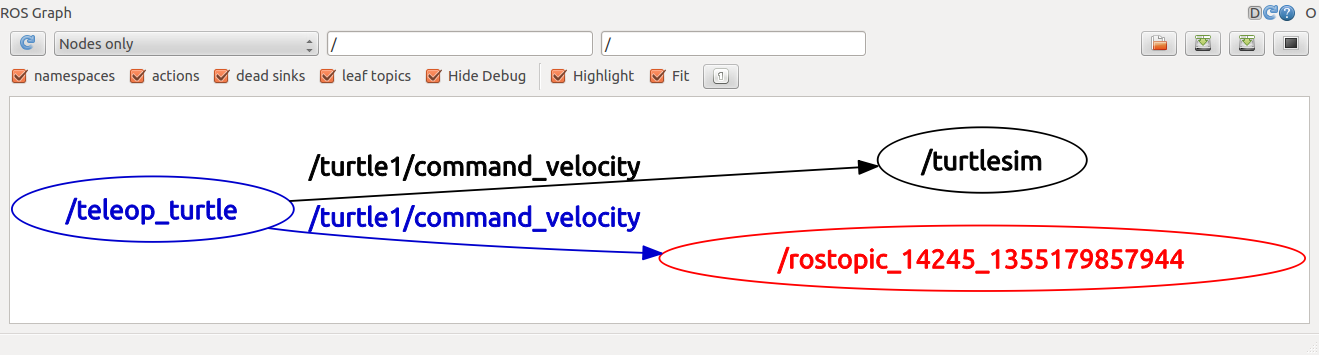
\includegraphics[width=.8\textwidth]{./img/ros/rqt_graph_echo.png}
\end{figure}
\end{frame}

\begin{frame}[fragile]{rostopic list}
\textbf{rostopic list} returns a list of all topics currently subscribed to and published.

\begin{lstlisting}[language=shell]
$ rostopic list -h # help message
...
$ rostopic list -v # This displays a verbose list of topics to publish to and subscribe to and their type.
Published topics:
 * /turtle1/color_sensor [turtlesim/Color] 1 publisher
 * /turtle1/cmd_vel [geometry_msgs/Twist] 1 publisher
 * /rosout [rosgraph_msgs/Log] 2 publishers
 * /rosout_agg [rosgraph_msgs/Log] 1 publisher
 * /turtle1/pose [turtlesim/Pose] 1 publisher

Subscribed topics:
 * /turtle1/cmd_vel [geometry_msgs/Twist] 1 subscriber
 * /rosout [rosgraph_msgs/Log] 1 subscriber
\end{lstlisting}
\end{frame}

\begin{frame}[fragile,allowframebreaks]{rostopic pub}
\textbf{rostopic pub} publishes data on to a topic currently advertised.

\begin{lstlisting}[language=syntax]
rostopic pub [topic] [msg_type] [args]
\end{lstlisting}

\begin{lstlisting}[language=shell]
$ rostopic pub -1 /turtle1/cmd_vel geometry_msgs/Twist -- '[2.0, 0.0, 0.0]' '[0.0, 0.0, 1.8]'
\end{lstlisting}

\begin{itemize}
 \item \texttt{-1} causes rostopic to only publish one message then exit.
 \item \texttt{/turtle1/cmd\_vel} is the name of the topic to publish to.
 \item \texttt{geometry\_msgs/Twist} is the message type to use when publishing to the topic.
 \item \texttt{--} tells the option parser that none of the following arguments is an option. This is required in cases where your arguments have a leading dash \texttt{-}, like negative numbers.
 \item \texttt{'[2.0, 0.0, 0.0]' '[0.0, 0.0, 1.8]'}, as noted before, a geometry\_msgs/Twist msg has two vectors of three floating point elements each: linear and angular. In this case, \texttt{'[2.0, 0.0, 0.0]'} becomes the linear value with x=2.0, y=0.0, and z=0.0, and '\texttt{[0.0, 0.0, 1.8]'} is the angular value with x=0.0, y=0.0, and z=1.8.
\end{itemize}

\framebreak

You may have noticed that the turtle has stopped moving; this is because the turtle requires a steady stream of commands at 1 Hz to keep moving. We can publish a steady stream of commands using rostopic pub -r command:

\begin{lstlisting}[language=shell]
$ rostopic pub /turtle1/cmd_vel geometry_msgs/Twist -r 1 -- '[2.0, 0.0, 0.0]' '[0.0, 0.0, -1.8]'
\end{lstlisting}

We can also look at what is happening in rqt\_graph. Press the refresh button in the upper-left. The rostopic pub node (here in red) is communicating with the rostopic echo node (here in green):
\begin{figure}
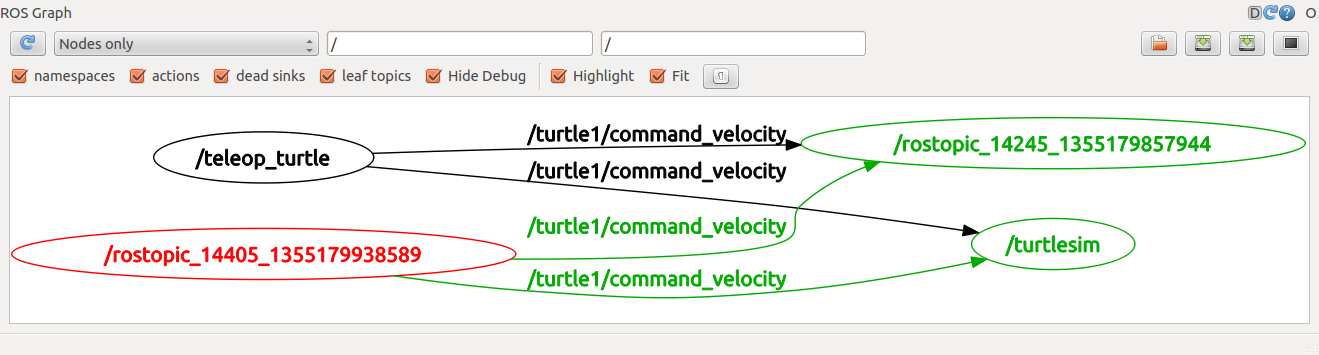
\includegraphics[width=.8\textwidth]{./img/ros/rqt_graph_pub.png}
\end{figure}
\end{frame}

\begin{frame}[fragile]{rostopic hz}
\textbf{rostopic hz} reports the rate at which data is published.

\begin{lstlisting}[language=syntax]
rostopic hz [topic]
\end{lstlisting}

\begin{lstlisting}[language=shell]
$ rostopic hz /turtle1/pose
subscribed to [/turtle1/pose]
average rate: 59.354
        min: 0.005s max: 0.027s std dev: 0.00284s window: 58
average rate: 59.459
        min: 0.005s max: 0.027s std dev: 0.00271s window: 118
average rate: 59.539
        min: 0.004s max: 0.030s std dev: 0.00339s window: 177
average rate: 59.492
        min: 0.004s max: 0.030s std dev: 0.00380s window: 237
average rate: 59.463
        min: 0.004s max: 0.030s std dev: 0.00380s window: 290
\end{lstlisting}
Now we can tell that the turtlesim is publishing data about our turtle at the rate of 60 Hz.
\end{frame}

\subsection{Writing a Simple Publisher and Subscriber (Python)}

\begin{frame}[fragile, allowframebreaks]{Writing the Publisher Node}
\textbf{Node} is the ROS term for an executable that is connected to the ROS network. Here we'll create the publisher (``talker'') node which will continually broadcast a message.

% FIXME REvisar kinetic 
\begin{lstlisting}[language=shell]
$ roscd my_first_package
$ mkdir scripts
$ cd scripts
$ wget https://raw.github.com/ros/ros_tutorials/kinetic-devel/rospy_tutorials/001_talker_listener/talker.py
$ chmod +x talker.py
\end{lstlisting}

\begin{lstlisting}[language=python]
#!/usr/bin/env python
# license removed for brevity
import rospy
from std_msgs.msg import String # import the std_msgs/String message type

def talker():
    pub = rospy.Publisher('chatter', String, queue_size=10)
    rospy.init_node('talker', anonymous=True)
    rate = rospy.Rate(10) # 10hz
    
    while not rospy.is_shutdown():
        hello_str = "hello world %s" % rospy.get_time()
        rospy.loginfo(hello_str)
        pub.publish(hello_str)
        rate.sleep()

if __name__ == '__main__':
    try:
        talker()
    except rospy.ROSInterruptException:
        pass
\end{lstlisting}

In ROS, nodes are uniquely named. If two nodes with the same name are launched, the previous one is kicked off. The \textbf{\texttt{anonymous=True}} flag means that rospy will choose a unique name for our 'talker' node so that multiple listeners can run simultaneously.

\framebreak

Then, edit the \texttt{catkin\_install\_python()} call in your CMakeLists.txt so it looks like the following:

\begin{lstlisting}[language=syntax]
catkin_install_python(PROGRAMS scripts/talker.py
  DESTINATION ${CATKIN_PACKAGE_BIN_DESTINATION}
)
\end{lstlisting}

Go to your catkin workspace and run catkin\_make:
\begin{lstlisting}[language=shell]
$ cd ~/catkin_ws
$ catkin_make
\end{lstlisting}
\end{frame}

% FIXME REvisar kinetic 
\begin{frame}[fragile,allowframebreaks]{Writing the Subscriber Node}
\begin{lstlisting}[language=shell]
$ roscd my_first_package/scripts/
$ wget https://raw.github.com/ros/ros_tutorials/kinetic-devel/rospy_tutorials/001_talker_listener/listener.py
$ chmod +x listener.py
\end{lstlisting}

\begin{lstlisting}[language=python]
#!/usr/bin/env python
import rospy
from std_msgs.msg import String

def callback(data):
    rospy.loginfo(rospy.get_caller_id() + "I heard %s", data.data)
    
def listener():
    rospy.init_node('listener', anonymous=True)
    rospy.Subscriber("chatter", String, callback)
    # spin() simply keeps python from exiting until this node is stopped
    rospy.spin()

if __name__ == '__main__':
    listener()
\end{lstlisting}

Then, edit the \texttt{catkin\_install\_python()} call in your CMakeLists.txt so it looks like the following:

\begin{lstlisting}[language=syntax]
catkin_install_python(PROGRAMS scripts/talker.py scripts/listener.py
  DESTINATION ${CATKIN_PACKAGE_BIN_DESTINATION}
)
\end{lstlisting}

Go to your catkin workspace and run \texttt{catkin\_make}:

\begin{lstlisting}[language=shell]
$ cd ~/catkin_ws
$ catkin_make
\end{lstlisting}
\end{frame}

\subsection{Examining the Simple Publisher and Subscriber}

\begin{frame}[fragile]{Running the Publisher}
Make sure that a roscore is up and running:
\begin{lstlisting}[language=shell]
$ roscore
\end{lstlisting}

Let's run talker node:
\begin{lstlisting}[language=shell]
$ rosrun my_first_package talker.py
[INFO] [WallTime: 1314931831.774057] hello world 1314931831.77
[INFO] [WallTime: 1314931832.775497] hello world 1314931832.77
[INFO] [WallTime: 1314931833.778937] hello world 1314931833.78
[INFO] [WallTime: 1314931834.782059] hello world 1314931834.78
[INFO] [WallTime: 1314931835.784853] hello world 1314931835.78
[INFO] [WallTime: 1314931836.788106] hello world 1314931836.79
\end{lstlisting}
\end{frame}

\begin{frame}[fragile]{Running the Subscriber}
Let's run listener node:
\begin{lstlisting}[language=shell]
$ rosrun my_first_package listener.py 
[INFO] [WallTime: 1314931969.258941] /listener_17657_1314931968795I heard hello world 1314931969.26
[INFO] [WallTime: 1314931970.262246] /listener_17657_1314931968795I heard hello world 1314931970.26
[INFO] [WallTime: 1314931971.266348] /listener_17657_1314931968795I heard hello world 1314931971.26
[INFO] [WallTime: 1314931972.270429] /listener_17657_1314931968795I heard hello world 1314931972.27
[INFO] [WallTime: 1314931973.274382] /listener_17657_1314931968795I heard hello world 1314931973.27
[INFO] [WallTime: 1314931974.277694] /listener_17657_1314931968795I heard hello world 1314931974.28
[INFO] [WallTime: 1314931975.283708] /listener_17657_1314931968795I heard hello world 1314931975.28
\end{lstlisting}
When you are done, press Ctrl-C to terminate both the listener and the talker.
\end{frame}

\subsection{Understanding ROS Services and Parameters}

\begin{frame}[fragile]{ROS services}
Services are another way that nodes can communicate with each other. Services allow nodes to send a \textbf{request} and receive a \textbf{response}.

\vspace{.1cm}
\textbf{rosservice}  has many commands that can be used on services:

\begin{lstlisting}[language=syntax]
rosservice list        # print information about active services
rosservice call        # call the service with the provided args
rosservice type        # print service type
rosservice find        # find services by service type
rosservice uri         # print service ROSRPC uri
\end{lstlisting}

  Now run roscore and turtlesim\_node to test some of them.
\end{frame}

\begin{frame}[fragile]{rosservice list}
\begin{lstlisting}[language=shell]
$ rosservice list
/clear
/kill
/reset
/rosout/get_loggers
/rosout/set_logger_level
/spawn
/teleop_turtle/get_loggers
/teleop_turtle/set_logger_level
/turtle1/set_pen
/turtle1/teleport_absolute
/turtle1/teleport_relative
/turtlesim/get_loggers
/turtlesim/set_logger_level
\end{lstlisting}
The list command shows us that the turtlesim\_node provides nine services: reset, clear, spawn, kill, turtle1/set\_pen, /turtle1/teleport\_absolute, /turtle1/teleport\_relative, turtlesim/get\_loggers, and turtlesim/set\_logger\_level.

\vspace{.1cm}
There are also two services related to the separate rosout node: /rosout/get\_loggers and /rosout/set\_logger\_level.
\end{frame}

\begin{frame}[fragile]{rosservice type}
\begin{lstlisting}[language=syntax]
rosservice type [service]
\end{lstlisting}
Let's find out what type the clear service is:
\begin{lstlisting}[language=shell]
$ rosservice type /clear
std_srvs/Empty
\end{lstlisting}
This service is empty, this means when the service call is made it takes no arguments (i.e. it sends no data when making a request and receives no data when receiving a response).
\end{frame}

\begin{frame}[fragile]{rosservice call}
\begin{lstlisting}[language=syntax]
rosservice call [service] [args]
\end{lstlisting}

Here we'll call with no arguments because the service is of type empty:
\begin{lstlisting}[language=shell]
$ rosservice call /clear
\end{lstlisting}
This does what we expect, it clears the background of the turtlesim\_node.

\vspace{.1cm}
Let's look at the case where the service has arguments:
\begin{lstlisting}[language=shell]
$ rosservice type /spawn | rossrv show
float32 x
float32 y
float32 theta
string name
---
string name
\end{lstlisting}
This service lets us spawn a new turtle at a given location and orientation. 
\begin{lstlisting}[language=shell]
$ rosservice call /spawn 2 2 0.2 "my_second_turtle"
name: my_second_turtle
\end{lstlisting}
\end{frame}

\begin{frame}[fragile]{Using rosparam}
\textbf{rosparam} allows you to store and manipulate data on the ROS Parameter Server. The Parameter Server can store integers, floats, boolean, dictionaries, and lists. rosparam uses the YAML markup language for syntax. 

\vspace{.1cm}
rosparam has many commands that can be used on parameters, as shown below:

\begin{lstlisting}[language=syntax]
rosparam set           # set parameter
rosparam get           # get parameter
rosparam load          # load parameters from file
rosparam dump          # dump parameters to file
rosparam delete        # delete parameter
rosparam list          # list parameter names
\end{lstlisting}
\end{frame}

\begin{frame}[fragile]{rosparam list}
\begin{lstlisting}[language=shell]
$ rosparam list
/background_b
/background_g
/background_r
/rosdistro
/roslaunch/uris/host_57aea0986fef__34309
/rosversion
/run_id
\end{lstlisting}
Here we can see that the turtlesim node has three parameters on the param server for background color.
\end{frame}

\begin{frame}[fragile,allowframebreaks]{rosparam set}
\begin{lstlisting}[language=syntax]
rosparam set [param_name]
rosparam get [param_name]
\end{lstlisting}
Here will change the red channel of the background color:

\begin{lstlisting}[language=shell]
$ rosparam set /background_r 150
\end{lstlisting}
This changes the parameter value, now we have to call the clear service for the parameter change to take effect:
\begin{lstlisting}[language=shell]
$ rosservice call /clear
\end{lstlisting}
Now our turtlesim shows a different background color.

\framebreak 

ROS  offers integrated measurement of the following parameters for every ROS connections (in rospy and roscpp).
\begin{itemize}
\item Period of messages by all publishers (average, maximum, standard deviation)
\item Age of messages, based on header timestamp (average, maximum, standard deviation)
\item Number of dropped messages
\item  Traffic volume (Bytes) 
\end{itemize}

\vspace{.2cm}
All measurements are performed on a window, that resizes automatically depending on the number of messages published.

\vspace{.2cm}
Note, that this parameter has to be set before you start your nodes.
\begin{lstlisting}[language=bash]
$ rosparam set enable_statistics true
\end{lstlisting}
\end{frame}

\begin{frame}[fragile]{rosparam get}
\begin{lstlisting}[language=syntax]
rosparam get [param_name]
\end{lstlisting}

Let's get the value of the green background channel:
\begin{lstlisting}[language=shell]
$ rosparam get /background_g 
86
\end{lstlisting}

We can also use rosparam get / to show us the contents of the entire Parameter Server.
\begin{lstlisting}[language=shell]
$ rosparam get /
background_b: 255
background_g: 86
background_r: 150
roslaunch:
  uris: {'aqy:51932': 'http://aqy:51932/'}
run_id: e07ea71e-98df-11de-8875-001b21201aa8
\end{lstlisting}
\end{frame}

\begin{frame}[fragile]{rosparam dump and rosparam load}
You may wish to store the Parameter Server contents in a file so that you can reload it at another time. This is easy using rosparam:

\begin{lstlisting}[language=syntax]
rosparam dump [file_name] [namespace]
rosparam load [file_name] [namespace]
\end{lstlisting}

Here we write all the parameters to the file params.yaml:
\begin{lstlisting}[language=shell]
$ rosparam dump params.yaml
\end{lstlisting}
You can even load these yaml files into new namespaces, e.g. copy:
\begin{lstlisting}[language=shell]
$ rosparam load params.yaml copy
$ rosparam get /copy/background_b
255
\end{lstlisting}
\end{frame}

\subsection{Using rqt\_console and roslaunch}

\begin{frame}[fragile]{Using rqt\_console and rqt\_logger\_level}
\begin{alertblock}{Prerequisites}
\begin{lstlisting}[language=shell]
$ sudo apt-get install ros-<distro>-rqt ros-<distro>-rqt-common-plugins ros-<distro>-turtlesim # Replace <distro> with the name of your ROS distribution (e.g. indigo, jade, kinetic, lunar...)
\end{lstlisting}
\end{alertblock}

\textbf{rqt\_console} attaches to ROS's logging framework to display output from nodes.
\begin{lstlisting}[language=shell]
$ rosrun rqt_console rqt_console
\end{lstlisting}

\textbf{rqt\_logger\_level} allows us to change the verbosity level (DEBUG, WARN, INFO, and ERROR) of nodes as they run.
\begin{lstlisting}[language=shell]
$ rosrun rqt_logger_level rqt_logger_level
\end{lstlisting}
Now let's look at the turtlesim output in rqt\_console and switch logger levels in rqt\_logger\_level as we use turtlesim.
\begin{lstlisting}[language=shell]
$ rosrun turtlesim turtlesim_node
\end{lstlisting}
\begin{lstlisting}[language=shell]
$ rostopic pub /turtle1/cmd_vel geometry_msgs/Twist -r 1 -- '{linear: {x: 2.0, y: 0.0, z: 0.0}, angular: {x: 0.0,y: 0.0,z: 0.0}}'
\end{lstlisting}
\end{frame}

\begin{frame}[fragile,allowframebreaks]{Using roslaunch}
\textbf{roslaunch} starts nodes as defined in a launch file.

\begin{lstlisting}[language=syntax]
roslaunch [package] [filename.launch]
\end{lstlisting}

First, we need to create a launch file:
\begin{lstlisting}[language=shell]
$ roscd my_first_package
$ mkdir launch # let's make a launch directory
$ cd launch
\end{lstlisting}

Now let's create a launch file called example.launch and paste the following:
\begin{lstlisting}[language=xml]
<launch>
  <node pkg="rqt_console" name="rqt_console" type="rqt_console"/>
  <node pkg="rqt_logger_level" name="rqt_logger_level" type="rqt_logger_level"/>
  <node pkg="turtlesim" name="my_turtle" type="turtlesim_node"/>
</launch>
\end{lstlisting}
Now we can launch it with roslaunch:
\begin{lstlisting}[language=shell]
$ roslaunch my_first_package example.launch
\end{lstlisting}
\end{frame}

\subsection{Using rosed to edit files in ROS}

\begin{frame}[fragile]{Using rosed}
\textbf{rosed} allows you to directly edit a file within a package by using the package name rather than having to type the entire path to the package.

\begin{lstlisting}[language=syntax]
$ rosed [package_name] [filename]
\end{lstlisting}

e.g.:
\begin{lstlisting}[language=syntax]
$ rosed roscpp Logger.msg
\end{lstlisting}

The default editor for rosed is vim. The more beginner-friendly editor nano is included with the default Ubuntu install. You can use it by editing your ~/.bashrc file to include:

\begin{lstlisting}[language=shell]
$ export EDITOR='nano -w'
\end{lstlisting}
\end{frame}

\subsection{Creating a ROS msg and srv}

\begin{frame}[fragile, allowframebreaks]{Creating a msg}

\textbf{msg} files are simple text files that describe the fields of a ROS message. They are used to generate source code for messages in different languages.

\vspace{.1cm}
Let's define a new msg in the my\_first\_package package:
\begin{lstlisting}[language=shell]
$ roscd my_first_package
$ mkdir msg
$ echo "int64 num" > msg/Num.msg
\end{lstlisting}

The example .msg file above contains only 1 line. You can, of course, create a more complex file by adding multiple elements, one per line, like this:

\begin{lstlisting}[language=shell]
string first_name
string last_name
uint8 age
uint32 score
\end{lstlisting}

We need to make sure that the msg files are turned into source code for C++, Python, and other languages:

\vspace{.1cm}
Open package.xml, and make sure these two lines are in it and uncommented:
\begin{lstlisting}[language=xml]
  <build_depend>message_generation</build_depend>
  <exec_depend>message_runtime</exec_depend>
\end{lstlisting}

Open CMakeLists.txt and add the message\_generation dependency to the find\_package call which already exists so that you can generate messages. You can do this by simply adding message\_generation to the list of COMPONENTS such that it looks like this:

\begin{lstlisting}[language=shell]
# Do not just add this to your CMakeLists.txt, modify the existing text to add message_generation before the closing parenthesis
find_package(catkin REQUIRED COMPONENTS
   roscpp
   rospy
   std_msgs
   message_generation
)
\end{lstlisting}

Also make sure you export the message runtime dependency.
\begin{lstlisting}[language=shell]
catkin_package(
  ...
  CATKIN_DEPENDS message_runtime ...
  ...)
\end{lstlisting}

Find the following block of code:
\begin{lstlisting}[language=shell]
# add_message_files(
#   FILES
#   Message1.msg
#   Message2.msg
# )
\end{lstlisting}

Uncomment it by removing the \# symbols and then replace the stand in Message*.msg files with your .msg file, such that it looks like this:

\begin{lstlisting}[language=shell]
add_message_files(
  FILES
  Num.msg
)
\end{lstlisting}
\end{frame}

\begin{frame}[fragile, allowframebreaks]{Creating a srv}
An \textbf{srv} file describes a service. It is composed of two parts: a request and a response.

\vspace{.1cm}
Let's use the package we just created to create a srv:

\begin{lstlisting}[language=shell]
$ roscd my_first_package
$ mkdir srv
\end{lstlisting}

Instead of creating a new srv definition by hand, we will copy an existing one from another package. For that, roscp is a useful commandline tool for copying files from one package to another.

\begin{lstlisting}[language=syntax]
$ roscp [package_name] [file_to_copy_path] [copy_path]
\end{lstlisting}

We can copy a service from the rospy\_tutorials package:
\begin{lstlisting}[language=shell]
$ roscp rospy_tutorials AddTwoInts.srv srv/AddTwoInts.srv
\end{lstlisting}

We need to make sure that the srv files are turned into source code for C++, Python, and other languages.

Unless you have done so already, open package.xml, and make sure these two lines are in it and uncommented:
\begin{lstlisting}[language=xml]
  <build_depend>message_generation</build_depend>
  <exec_depend>message_runtime</exec_depend>
\end{lstlisting}

Unless you have done so already for messages in the previous step, add the message\_generation dependency to generate messages in CMakeLists.txt:

\begin{lstlisting}[language=shell]
# Do not just add this line to your CMakeLists.txt, modify the existing line
find_package(catkin REQUIRED COMPONENTS
  roscpp
  rospy
  std_msgs
  message_generation
)
\end{lstlisting}

Despite its name, message\_generation works for both msg and srv.

Remove \# to uncomment the following lines:
\begin{lstlisting}[language=shell]
# add_service_files(
#   FILES
#   Service1.srv
#   Service2.srv
# )
\end{lstlisting}

And replace the placeholder Service*.srv files for your service files:
\begin{lstlisting}[language=shell]
add_service_files(
  FILES
  AddTwoInts.srv
)
\end{lstlisting}
\end{frame}

\begin{frame}[fragile, allowframebreaks]{Common step for msg and srv}
We must ensure the generate\_messages() function is called. you need to uncomment these lines:
\begin{lstlisting}[language=shell]
# generate_messages(
#   DEPENDENCIES
#   std_msgs
# )
\end{lstlisting}

so it looks like:
\begin{lstlisting}[language=shell]
generate_messages(
  DEPENDENCIES
  std_msgs
)
\end{lstlisting}

Now that we have made some new messages we need to make our package again:

\begin{lstlisting}[language=shell]
# In your catkin workspace
$ roscd my_first_package
$ cd ../..
$ catkin_make install
\end{lstlisting}

\framebreak
Any .msg file in the msg directory will generate code for use in all supported languages.
\begin{itemize}
 \item The C++ message header file will be generated in ~/catkin\_ws/devel/include/my\_first\_package/. 
 \item The Python script will be created in ~/catkin\_ws/devel/lib/python2.7/dist-packages/my\_first\_package/msg.
 \item The lisp file appears in ~/catkin\_ws/devel/share/common-lisp/ros/my\_first\_package/msg/.
\end{itemize}

\vspace{.1cm}
Similarly, any .srv files in the srv directory will have generated code in supported languages.
\begin{itemize}
  \item For C++, this will generate header files in the same directory as the message header files. 
  \item For Python and Lisp, there will be an 'srv' folder beside the 'msg' folders.
\end{itemize}
\end{frame}

\begin{frame}[fragile]{rosmsg show}
Let's make sure that ROS can see our msg using the \textbf{rosmsg show} command.
\begin{lstlisting}[language=syntax]
rosmsg show [message type]
\end{lstlisting}

e.g.:
\begin{lstlisting}[language=shell]
$ rosmsg show Num
[my_first_package/Num]:
int64 num
\end{lstlisting}
\end{frame}

\begin{frame}[fragile]{rossrv show}
Let's make sure that ROS can see our srv using the \textbf{rossrv show} command.

\begin{lstlisting}[language=syntax]
$ rossrv show <service type>
\end{lstlisting}

e.g.:
\begin{lstlisting}[language=shell]
$ rossrv show AddTwoInts
[my_first_package/AddTwoInts]:
int64 a
int64 b
---
int64 sum

[rospy_tutorials/AddTwoInts]:
int64 a
int64 b
---
int64 sum
\end{lstlisting}
\end{frame}

\subsection{Writing a Simple Service and Client (Python)}

\begin{frame}[fragile, allowframebreaks]{Writing a Service Node}
We'll create the service ``add\_two\_ints\_server'' node which will receive two ints and return the sum.

\begin{lstlisting}[language=shell]
$ roscd my_first_package
\end{lstlisting}

Create scripts/add\_two\_ints\_server.py and paste the following inside it:

\begin{lstlisting}[language=python]
#!/usr/bin/env python

from my_first_package.srv import *
import rospy

def handle_add_two_ints(req):
    print "Returning [%s + %s = %s]"%(req.a, req.b, (req.a + req.b))
    return AddTwoIntsResponse(req.a + req.b)

def add_two_ints_server():
    rospy.init_node('add_two_ints_server')
    s = rospy.Service('add_two_ints', AddTwoInts, handle_add_two_ints)
    print "Ready to add two ints."
    rospy.spin()

if __name__ == "__main__":
    add_two_ints_server()
\end{lstlisting}

\texttt{rospy.Service(...}) declares a new service named add\_two\_ints with the AddTwoInts service type. All requests are passed to handle\_add\_two\_ints function. handle\_add\_two\_ints is called with instances of AddTwoIntsRequest and returns instances of AddTwoIntsResponse.

\vspace{.1cm}
Don't forget to make the node executable:
\begin{lstlisting}[language=shell]
chmod +x scripts/add_two_ints_server.py
\end{lstlisting}
\end{frame}

\begin{frame}[fragile,allowframebreaks]{Writing the Client Node}
Create the scripts/add\_two\_ints\_client.py file within the my\_first\_package package and paste the following inside it:

\begin{lstlisting}[language=python]
#!/usr/bin/env python

import sys
import rospy
from my_first_package.srv import *

def add_two_ints_client(x, y):
    rospy.wait_for_service('add_two_ints')
    try:
        add_two_ints = rospy.ServiceProxy('add_two_ints', AddTwoInts)
        resp1 = add_two_ints(x, y)
        return resp1.sum
    except rospy.ServiceException, e:
        print "Service call failed: %s"%e

def usage():
    return "%s [x y]"%sys.argv[0]

if __name__ == "__main__":
    if len(sys.argv) == 3:
        x = int(sys.argv[1])
        y = int(sys.argv[2])
    else:
        print usage()
        sys.exit(1)
    print "Requesting %s+%s"%(x, y)
    print "%s + %s = %s"%(x, y, add_two_ints_client(x, y))
\end{lstlisting}

Don't forget to make the node executable:
\begin{lstlisting}[language=shell]
$ chmod +x scripts/add_two_ints_client.py

\end{lstlisting}
Go to your catkin workspace and run catkin\_make.
\begin{lstlisting}[language=shell]
$ cd ~/catkin_ws
$ catkin_make
\end{lstlisting}
\end{frame}

\subsection{Examining the Simple Service and Client}

\begin{frame}[fragile]{Running the Service and the Client}
Let's start by running the service:
\begin{lstlisting}[language=shell]
$ rosrun my_first_package add_two_ints_server.py
\end{lstlisting}
You should see something similar to:
\begin{lstlisting}[language=shell]
Ready to add two ints.
\end{lstlisting}

Now let's run the client with the necessary arguments:
\begin{lstlisting}[language=shell]
$ rosrun my_first_package add_two_ints_client.py 1 3  (Python) 
\end{lstlisting}
You should see something similar to:
\begin{lstlisting}[language=shell]
Requesting 1+3
1 + 3 = 4
\end{lstlisting}
\end{frame}

\subsection{Recording and playing back data}

\begin{frame}[fragile, allowframebreaks]{Recording data (creating a bag file)}
First, execute the following commands in separate terminals:
\begin{lstlisting}[language=shell]
$ roscore
\end{lstlisting}
\begin{lstlisting}[language=shell]
$ rosrun turtlesim turtlesim_node 
\end{lstlisting}
\begin{lstlisting}[language=shell]
$ rosrun turtlesim turtle_teleop_key
\end{lstlisting}
\begin{lstlisting}[language=shell]
$ rostopic list -v
Published topics:
 * /turtle1/color_sensor [turtlesim/Color] 1 publisher
 * /turtle1/cmd_vel [geometry_msgs/Twist] 1 publisher
 * /rosout [rosgraph_msgs/Log] 2 publishers
 * /rosout_agg [rosgraph_msgs/Log] 1 publisher
 * /turtle1/pose [turtlesim/Pose] 1 publisher

Subscribed topics:
 * /turtle1/cmd_vel [geometry_msgs/Twist] 1 subscriber
 * /rosout [rosgraph_msgs/Log] 1 subscriber
\end{lstlisting}

We now will record the published data. In a new terminal:
\begin{lstlisting}[language=shell]
$ mkdir ~/bagfiles
$ cd ~/bagfiles
$ rosbag record -a # record all published topics
\end{lstlisting}
Move back to the terminal window with turtle\_teleop\_key and move the turtle around for 10 or so seconds. In the window running rosbag record exit with a Ctrl-C. Now examine the contents of the directory $\sim$/bagfiles. You should see a file with a name that begins with the year, date, and time and the suffix .bag.
\end{frame}

\begin{frame}[fragile, allowframebreaks]{Examining and playing the bag file}
Execute the following command from the bagfiles directory:
\begin{lstlisting}[language=shell]
$ cd ~/bagfiles
$ rosbag info <your bagfile>
path:        2014-12-10-20-08-34.bag
version:     2.0
duration:    1:38s (98s)
start:       Dec 10 2014 20:08:35.83 (1418270915.83)
end:         Dec 10 2014 20:10:14.38 (1418271014.38)
size:        865.0 KB
messages:    12471
compression: none [1/1 chunks]
types:       geometry_msgs/Twist [9f195f881246fdfa2798d1d3eebca84a]
             rosgraph_msgs/Log   [acffd30cd6b6de30f120938c17c593fb]
             turtlesim/Color     [353891e354491c51aabe32df673fb446]
             turtlesim/Pose      [863b248d5016ca62ea2e895ae5265cf9]
topics:      /rosout                    4 msgs    : rosgraph_msgs/Log   (2 connections)
             /turtle1/cmd_vel         169 msgs    : geometry_msgs/Twist
             /turtle1/color_sensor   6149 msgs    : turtlesim/Color    
             /turtle1/pose           6149 msgs    : turtlesim/Pose
\end{lstlisting}

\framebreak
Now, let's replay the bag file to reproduce behavior in the running system. First kill the teleop program that may be still running from the previous section. Leave turtlesim running. 
\begin{lstlisting}[language=shell]
$ rosbag play <your bagfile>
[ INFO] [1418271315.162885976]: Opening 2014-12-10-20-08-34.bag

Waiting 0.2 seconds after advertising topics... done.

Hit space to toggle paused, or 's' to step.
\end{lstlisting}

To change the rate of publishing by a specified factor:
\begin{lstlisting}[language=shell]
$ rosbag play -r 2 <your bagfile>
\end{lstlisting}
\end{frame}

\begin{frame}[fragile]{Recording a subset of the data}
The \textbf{rosbag record} command supports logging only particular topics.

\begin{lstlisting}[language=shell]
$ rosrun turtlesim turtlesim_node 
\end{lstlisting}
\begin{lstlisting}[language=shell]
$ rosrun turtlesim turtle_teleop_key
\end{lstlisting}
\begin{lstlisting}[language=shell]
$ rosbag record -O subset /turtle1/cmd_vel /turtle1/pose # move turtle and then stop this
\end{lstlisting}
\begin{lstlisting}[language=shell]
$ rosbag info subset.bag # after stop recording
path:        subset.bag
version:     2.0
duration:    12.6s
start:       Dec 10 2014 20:20:49.45 (1418271649.45)
end:         Dec 10 2014 20:21:02.07 (1418271662.07)
size:        68.3 KB
messages:    813
compression: none [1/1 chunks]
types:       geometry_msgs/Twist [9f195f881246fdfa2798d1d3eebca84a]
             turtlesim/Pose      [863b248d5016ca62ea2e895ae5265cf9]
topics:      /turtle1/cmd_vel    23 msgs    : geometry_msgs/Twist
             /turtle1/pose      790 msgs    : turtlesim/Pose
\end{lstlisting}
\end{frame}

\subsection{Getting started with roswtf}

\begin{frame}[fragile]{Checking your installation}
\textbf{roswtf} examines your system to try and find problems. Before you start, please make sure your roscore is NOT running.

\begin{lstlisting}[language=shell]
$ roscd rosmaster
$ roswtf
Package: rosmaster
================================================================================
Static checks summary:

No errors or warnings
================================================================================

ROS Master does not appear to be running.
Online graph checks will not be run.
ROS_MASTER_URI is [http://localhost:11311]
\end{lstlisting}

\begin{alertblock}{To check if roscore is still running}
\begin{lstlisting}[language=shell]
$ ps -ef | grep -i rosmaster
00:00:00 /usr/bin/python /opt/ros/noetic/bin/rosmaster 
\end{lstlisting}
\end{alertblock}
\end{frame}

\begin{frame}[fragile]{Trying it online (roscore running)}
\begin{lstlisting}[language=shell]
$ roscd
$ roswtf
No package or stack in context
======================================================
Static checks summary:

No errors or warnings
======================================================
Beginning tests of your ROS graph. These may take awhile...
analyzing graph...
... done analyzing graph
running graph rules...
... done running graph rules

Online checks summary:

Found 1 warning(s).
Warnings are things that may be just fine, but are sometimes at fault

WARNING The following node subscriptions are unconnected:
 * /rosout:
   * /rosout
\end{lstlisting}
\end{frame}

%\subsection{Creating a ROS package by hand}

\subsection{Action Clients and Servers}

\begin{frame}[fragile,allowframebreaks]{Action Clients and Servers}
 \begin{itemize}
  \item The actionlib stack provides a standardized interface for interfacing with \textbf{preemptable tasks}. Examples of this include:
   \begin{itemize}
    \item moving the base to a target location, 
    \item performing a laser scan and returning the resulting point cloud, 
    \item detecting the handle of a door, 
    \item etc.
\end{itemize}     
  \item The \textbf{ActionClient} and \textbf{ActionServer} communicate via a \textbf{ROS Action Protocol}, which is built on top of ROS messages. 
   \begin{itemize}
    \item The client and server then provide a simple API for users
     \begin{itemize}
      \item to request goals (on the client side) 
      \item or to execute goals (on the server side) via function calls and callbacks.
     \end{itemize}         
   \end{itemize}       
   \begin{figure}
    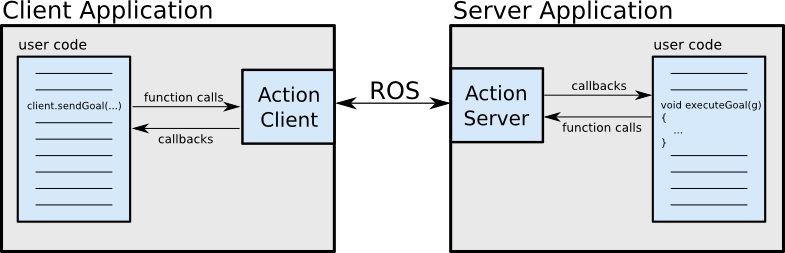
\includegraphics[width=.7\textwidth]{./img/ros/actionlib.png}
   \end{figure}
  \item Before writing an action we need to define the \textbf{goal}, \textbf{result}, and \textbf{feedback messages}. 

%  \item \texttt{actionlib\_tutorials} is a series of tutorials for using the actionlib client API. 
%  \item You can browse these tutorials by installing \texttt{common\_tutorials} and roscd-ing to the \texttt{actionlib\_tutorials} package, i.e.:
%\begin{lstlisting}[language=shell]
%$ apt-get install ros-noetic-common-tutorials
%$ roscd actionlib_tutorials
%\end{lstlisting}
  
  \item Before starting, create a sandbox package with the following dependencies:
\begin{lstlisting}[language=shell]
$ cd %YOUR_CATKIN_WORKSPACE%/src
$ catkin_create_pkg actionlib_tutorials actionlib message_generation roscpp rospy std_msgs actionlib_msgs
\end{lstlisting}
  
 \end{itemize}
\end{frame}

\begin{frame}[fragile,allowframebreaks]{Creating the Action Messages}
 \begin{itemize}
  \item The action messages are generated automatically from the \texttt{.action} file. 
   \begin{itemize}
    \item This file defines the type and format of the goal, result, and feedback topics for the action. 
    \item E.g. create \texttt{actionlib\_tutorials/action/Fibonacci.action} as follows:
   \end{itemize}  
\begin{lstlisting}[language=syntax]  
#goal definition
int32 order
---
#result definition
int32[] sequence
---
#feedback
int32[] sequence
\end{lstlisting}  

  \framebreak
  
  \item To automatically generate the message files during the make process, a few things need to be added to \texttt{CMakeLists.txt}.
   \begin{enumerate}
    \item add the \texttt{actionlib\_msgs} package to the \texttt{find\_package} macro's argument like this (if you used \texttt{catkin\_create\_package} to generate \texttt{CMakeLists.txt}, this may already have been added):
\begin{lstlisting}[language=syntax]
find_package(catkin REQUIRED COMPONENTS actionlib_msgs)  
\end{lstlisting}  
     \begin{itemize}
      \item Note that CMake needs to \texttt{find\_package} \texttt{actionlib\_msgs} (\texttt{message\_generation} does not need to be listed explicitly, it is referenced implicitly by \texttt{actionlib\_msgs}).
     \end{itemize}
     
    \item use the \texttt{add\_action\_files} macro to declare the actions you want to be generated:
\begin{lstlisting}[language=syntax]  
add_action_files(
  DIRECTORY action
  FILES Fibonacci.action
)
\end{lstlisting}  

    \framebreak

    \item call the \texttt{generate\_messages} macro, not forgetting the dependencies on \texttt{actionlib\_msgs} and other message packages like \texttt{std\_msgs}:
\begin{lstlisting}[language=syntax]  
generate_messages(
  DEPENDENCIES actionlib_msgs std_msgs  # Or other packages containing msgs
)
\end{lstlisting}  

    \item add \texttt{actionlib\_msgs} to \texttt{catkin\_package} macro like this:
\begin{lstlisting}[language=syntax]  
catkin_package(
  CATKIN_DEPENDS actionlib_msgs
)
\end{lstlisting}  
    \begin{itemize}
     \item \texttt{catkin\_package} also specifies only \texttt{CATKIN\_DEPEND} to \texttt{actionlib\_msgs}. The transitive dependency on \texttt{message\_runtime} is happening automatically.
    \end{itemize}
   \end{enumerate}

  \framebreak
  
  \item You have to setup your \texttt{package.xml}, since we are generating messages you have to declare on the manifest file that at run time you have to generate messages:
\begin{lstlisting}[language=syntax]  
<exec_depend>message_generation</exec_depend>
\end{lstlisting}  

 \item Now by following, automatically generate msg files of your action files:
\begin{lstlisting}[language=shell]  
$ cd ../.. # Go back to the top level of your catkin workspace
$ catkin_make
...
$ ls devel/share/actionlib_tutorials/msg/
FibonacciActionFeedback.msg  FibonacciAction.msg        FibonacciFeedback.msg
FibonacciResult.msg          FibonacciActionGoal.msg    FibonacciActionResult.msg  FibonacciGoal.msg
$ ls devel/include/actionlib_tutorials/
FibonacciActionFeedback.h  FibonacciAction.h        FibonacciFeedback.h  FibonacciResult.h
FibonacciActionGoal.h      FibonacciActionResult.h  FibonacciGoal.h
\end{lstlisting}   
 \end{itemize} 
\end{frame}

\begin{frame}[fragile,allowframebreaks]{Writing a Simple Action Server (Python)}
\texttt{fibonacci\_server.py} implements a python action server for the Fibonacci action. Place it in \texttt{actionlib\_tutorials/simple\_action\_servers}.

\begin{lstlisting}[language=python]  
#!/usr/bin/env python3
import rospy
from actionlib import SimpleActionServer
from actionlib_tutorials.msg import FibonacciAction, FibonacciFeedback, FibonacciResult

class FibonacciAction(object):
    # Create messages that are used to publish feedback/result.
    _feedback = FibonacciFeedback()
    _result = FibonacciResult()

    def __init__(self, name):
        self._action_name = name
        self._as = SimpleActionServer(self._action_name, FibonacciAction,
                                      execute_cb=self.execute_cb, auto_start = False)
        self._as.start()
        
    # This is the execute callback function that we'll run everytime a new goal is received.
    def execute_cb(self, goal):
        # Helper variables.
        r = rospy.Rate(1)
        success = True
        
        # Append the seeds for the fibonacci sequence.
        self._feedback.sequence = []
        self._feedback.sequence.append(0)
        self._feedback.sequence.append(1)
        
        # Publish info to the console for the user.
        rospy.loginfo('%s: Executing, creating fibonacci sequence 
                      of order %i with seeds %i, %i'
                      % (self._action_name, goal.order, 
                      self._feedback.sequence[0], self._feedback.sequence[1]))

        # Start executing the action.
        for i in range(1, goal.order):
            # Check that preempt has not been requested by the client.
            if self._as.is_preempt_requested():
                rospy.loginfo('%s: Preempted' % self._action_name)
                self._as.set_preempted() # Signal that the action has been preempted.
                success = False
                break

            self._feedback.sequence.append(self._feedback.sequence[i]
                                           + self._feedback.sequence[i-1])
            self._as.publish_feedback(self._feedback) # Publish the feedback.
            r.sleep()
            
        if success:
            self._result.sequence = self._feedback.sequence
            rospy.loginfo('%s: Succeeded' % self._action_name)
            self._as.set_succeeded(self._result) # Notify the action client 
                                                 #   that the goal is complete.

if __name__ == '__main__':
    rospy.init_node('fibonacci')
    server = FibonacciAction(rospy.get_name())
    rospy.spin()
\end{lstlisting} 

\framebreak
To compile and run the action server:
 \begin{enumerate}
  \item Compile to generate shell config files:
\begin{lstlisting}[language=shell]  
$ cd %TOPDIR_YOUR_CATKIN_WORKSPACE%
$ catkin_make
...
$ source devel/setup.bash
\end{lstlisting} 
  \item Run:
\begin{lstlisting}[language=shell]  
$ roscore
\end{lstlisting} 
  \item Then on a new terminal, the following command will run the action server.
\begin{lstlisting}[language=shell]  
$ rosrun actionlib_tutorials fibonacci_server.py
\end{lstlisting} 
 \end{enumerate}
\end{frame}

\begin{frame}[fragile,allowframebreaks]{Writing a Simple Action Client (Python)}
\texttt{fibonacci\_client.py} implements a python action client for the Fibonacci action.

\begin{lstlisting}[language=python]  
#!/usr/bin/env python3
import rospy
from actionlib import SimpleActionClient
from actionlib_tutorials.msg import FibonacciAction, FibonacciGoal, FibonacciResult

def fibonacci_client():
    # Creates the SimpleActionClient, passing the type of the action
    #   (FibonacciAction) to the constructor.
    client = SimpleActionClient('fibonacci', FibonacciAction)

    # Waits until the action server has started up and started listening for goals.
    client.wait_for_server()

    # Creates a goal to send to the action server.
    goal = FibonacciGoal(order=20)

    # Sends the goal to the action server.
    client.send_goal(goal)

    # Waits for the server to finish performing the action.
    client.wait_for_result()

    # Prints out the result of executing the action
    return client.get_result()  # A FibonacciResult

if __name__ == '__main__':
    try:
        # Initializes a rospy node so that the SimpleActionClient can
        #   publish and subscribe over ROS.
        rospy.init_node('fibonacci_client_py')
        result = fibonacci_client()
        print("Result:", ', '.join([str(n) for n in result.sequence]))
    except rospy.ROSInterruptException:
        print("program interrupted before completion", file=sys.stderr)
\end{lstlisting} 

\framebreak
Start the client. It will start up, send a goal to the server, wait for the goal to complete, and then exit.
\begin{lstlisting}[language=shell]  
$ rosrun actionlib_tutorials fibonacci_client.py
\end{lstlisting} 

\begin{itemize}
 \item Before running the client, roscore and Action server must be already running.
\end{itemize}
\end{frame}





%%% ESTA PARTE ES PARA EXPLICAR EL TURLTLEBOT3
\section{Managing a real robot: TurtleBot 3}%http://wiki.ros.org/Robots/TurtleBot

\begin{frame}{TurtleBot3}
\begin{itemize}
 \item TurtleBot is a ROS standard platform robot.
 \item There are 3 versions of the TurtleBot series. 
  \begin{enumerate}
   \item TurtleBot1 was developed by Tully (Platform Manager at Open Robotics) and Melonee (CEO of Fetch Robotics) from Willow Garage on top of the iRobot’s Roomba-based research robot, Create, for ROS deployment. It was developed in 2010 and has been on sale since 2011. 
   \item In 2012, TurtleBot2 was developed by Yujin Robot based on the research robot, iClebo Kobuki. 
   \item In 2017, TurtleBot3 was developed with features to supplement the lacking functions of its predecessors, and the demands of users. The TurtleBot3 adopts ROBOTIS smart actuator Dynamixel for driving.
  \end{enumerate}   
 \item TurtleBot3 is a small, affordable, programmable, ROS-based mobile robot for use in education, research, hobby, and product prototyping.
 \item TurtleBot3 is a collaboration project among Open Robotics, ROBOTIS, and more partners.
\end{itemize}
\begin{block}{TurtleBot3 Introduction Video}
\url{https://youtu.be/9OC3J53RUsk}
\end{block}
\end{frame}

\subsection{Turtlebot Installation}

\begin{frame}[fragile, allowframebreaks]{PC installation}
Install ROS on Remote PC:
\begin{lstlisting}[language=shell]
$ sudo apt update
$ sudo apt upgrade
$ wget https://raw.githubusercontent.com/ROBOTIS-GIT/robotis_tools/master/install_ros_noetic.sh
$ chmod 755 ./install_ros_noetic.sh 
$ bash ./install_ros_noetic.sh
\end{lstlisting}

Install Dependent ROS Packages:
\begin{lstlisting}[language=shell]
$ sudo apt-get install ros-noetic-joy ros-noetic-teleop-twist-joy ros-noetic-teleop-twist-keyboard ros-noetic-laser-proc ros-noetic-rgbd-launch ros-noetic-rosserial-arduino ros-noetic-rosserial-python ros-noetic-rosserial-client ros-noetic-rosserial-msgs ros-noetic-amcl ros-noetic-map-server ros-noetic-move-base ros-noetic-urdf ros-noetic-xacro ros-noetic-compressed-image-transport ros-noetic-rqt* ros-noetic-rviz ros-noetic-gmapping ros-noetic-navigation ros-noetic-interactive-markers ros-noetic-turtlebot3-msgs ros-noetic-turtlebot3-description ros-noetic-dynamixel-sdk ros-noetic-turtlebot3
$ cd ~/catkin_ws && catkin_make
\end{lstlisting}

Network configuration. Add the following lines to your $\sim$/.bashrc file:
\begin{lstlisting}[language=shell]
export TURTLEBOT3_MODEL=burger
export ROS_MASTER_URI=http://localhost:11311
export ROS_HOSTNAME=localhost
\end{lstlisting}
Usually, ROS\_MASTER\_URI and ROS\_HOSTNAME doesn't look like this. An usual configuration would be like this:
\begin{figure}
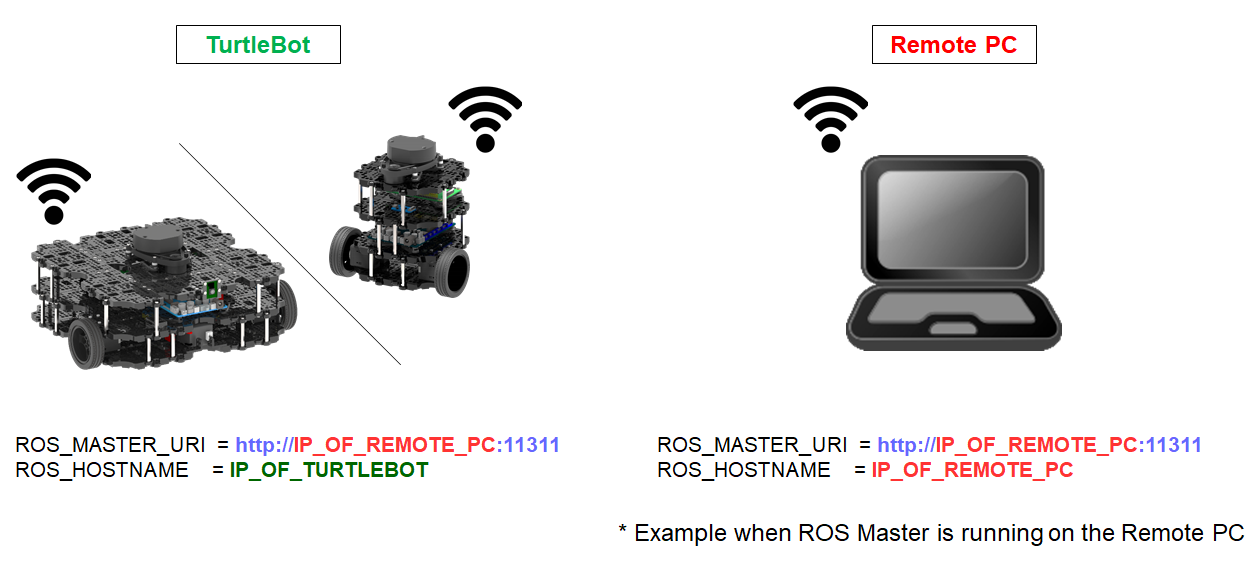
\includegraphics[width=.65\textwidth]{./img/ros/network_configuration.png}
\end{figure}
\end{frame}

\begin{frame}{TurtleBotPC and OpenCR installation}
To finish your installation you also need to:
\begin{itemize}
 \item Install Linux, ROS and hardware related packages to control the TurtleBot3 on your TurtleBot PC.
  \begin{itemize}
   \item \url{http://emanual.robotis.com/docs/en/platform/turtlebot3/sbc_setup/}
  \end{itemize}
  \begin{figure}
   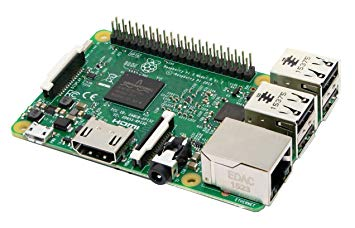
\includegraphics[height=1.7cm]{./img/ros/raspberry.jpg}
  \end{figure}
 \item Upload latest firmware of TurtleBot3 to embedded board OpenCR.
  \begin{itemize}
   \item \url{http://emanual.robotis.com/docs/en/platform/turtlebot3/hardware_setup/}
  \end{itemize}
  \begin{figure}
   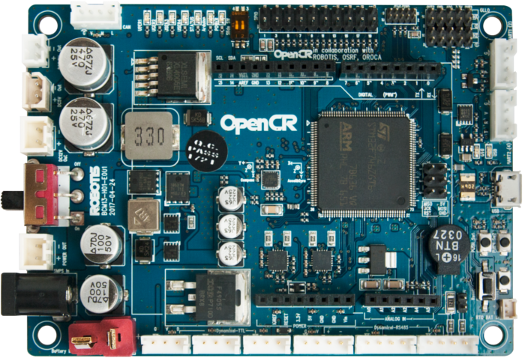
\includegraphics[height=1.7cm]{./img/ros/opencr.png}
  \end{figure}
\end{itemize}
\end{frame}

\subsection{Turtlebot Simulation}

\begin{frame}[fragile]{TurtleBot3 Simulation Installation}

\begin{lstlisting}[language=shell]
$ sudo apt-get install ros-noetic-joy ros-noetic-teleop-twist-joy ros-noetic-teleop-twist-keyboard ros-noetic-laser-proc ros-noetic-rgbd-launch ros-noetic-rosserial-arduino ros-noetic-rosserial-python ros-noetic-rosserial-client ros-noetic-rosserial-msgs ros-noetic-amcl ros-noetic-map-server ros-noetic-move-base ros-noetic-urdf ros-noetic-xacro ros-noetic-compressed-image-transport ros-noetic-rqt* ros-noetic-rviz ros-noetic-gmapping ros-noetic-navigation ros-noetic-interactive-markers ros-noetic-turtlebot3-msgs ros-noetic-turtlebot3-description
$ export TURTLEBOT3_MODEL=burger
$ cd ~/catkin_ws/src/
$ git clone -b noetic-devel https://github.com/ROBOTIS-GIT/turtlebot3_simulations.git
$ cd ~/catkin_ws && catkin_make
\end{lstlisting}

% The turtlebot3\_simulation metapackage requires turtlebot3 metapackage and turtlebot3\_msgs package as a prerequisite. 

% \vspace{.1cm}
% The turtlebot3\_fake is a very simple simulation node that can be run without having an actual robot. To launch the virtual robot, execute the turtlebot3\_fake.launch file in the turtlebot3\_fake package:
% \begin{lstlisting}[language=shell]
% $ roslaunch turtlebot3_fake turtlebot3_fake.launch
% \end{lstlisting}

% You can even control the virtual TurtleBot3 in RViz with a teleoperation node.
% \begin{lstlisting}[language=shell]
% $ roslaunch turtlebot3_teleop turtlebot3_teleop_key.launch
% \end{lstlisting}
\end{frame}

\begin{frame}[fragile]{TurtleBot3 Simulation using Gazebo}
The following command can be used to test the virtual TurtleBot3 on the empty world of the gazebo default environment.
\begin{lstlisting}[language=shell]
$ roslaunch turtlebot3_gazebo turtlebot3_empty_world.launch
\end{lstlisting}

TurtleBot3 world is a map consists of simple objects that makes up the shape of TurtleBot3 symbol. TurtleBot3 world is mainly used for testing such as SLAM and Navigation.  
\begin{lstlisting}[language=shell]
$ roslaunch turtlebot3_gazebo turtlebot3_world.launch
\end{lstlisting}

TurtleBot3 House is a map made with house drawings. It is suitable for testing related to more complex task performance.
\begin{lstlisting}[language=shell]
$ roslaunch turtlebot3_gazebo turtlebot3_house.launch
\end{lstlisting}

In order to control a TurtleBot3 with a keyboard, launch teleoperation feature with below command in a new terminal window.
\begin{lstlisting}[language=shell]
$ roslaunch turtlebot3_teleop turtlebot3_teleop_key.launch
\end{lstlisting}

RViz visualizes published topics while simulation is running. 
\begin{lstlisting}[language=shell]
$ roslaunch turtlebot3_gazebo turtlebot3_gazebo_rviz.launch
\end{lstlisting}
\end{frame}
%
%% ESTA PARTE ES PARA EXPLICAR EL SUMMIT

\section{Managing a real robot: Summit XL}
\begin{frame}{Summit XL}
\begin{figure}
    \centering
    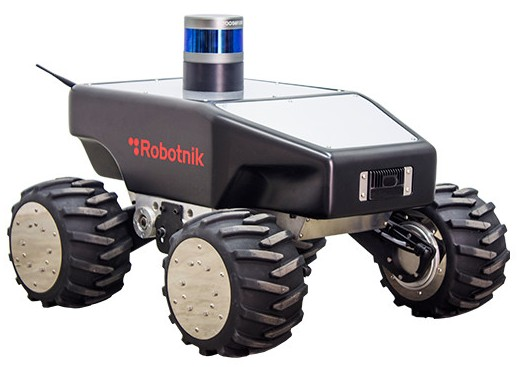
\includegraphics[scale=0.5]{img/ros/summit-xl.jpg}
\end{figure}
\end{frame}

\subsection{Summit Installation}
\label{subsec:summit_installation}

\begin{frame}[fragile]{PC installation}
\begin{enumerate}
    \item Install ROS noetic on PC or use a Docker image.
    \item Network configuration:
    \begin{itemize}
        \item Connect to the router of the robot (SSID: SUMMIT)
        \item Add to the /etc/hosts file the following data:
\begin{lstlisting}[language=shell]
192.168.0.200   shl00-230623aa
\end{lstlisting}
        \item Configure ROS\_MASTER and ROS\_IP parameters:
\begin{lstlisting}[language=shell]
export ROS_MASTER_URI=http://shl00-230623aa:11311
export ROS_IP=<IP provided by the router of the robot>
\end{lstlisting}
    
    \end{itemize}
\end{enumerate}
\end{frame}

\subsection{Summit Simulation}

\begin{frame}[fragile]{Summit Simulation in PC}
Install the repository of Robotnik in the workspace:
\begin{lstlisting}[language=shell]
$ cd catkin_ws
$ sudo apt-get install -y python3-vcstool
$ vcs import --input https://raw.githubusercontent.com/RobotnikAutomation/summit_xl_sim/noetic-devel/repos/summit_xl_sim_devel.repos
$ rosdep install --from-paths src --ignore-src --skip-keys="summit_xl_robot_control marker_mapping robotnik_locator robotnik_pose_filter robotnik_gazebo_elevator" -y -r
$ catkin_make
$ source devel/setup.bash
\end{lstlisting}

Launch the simulation:
\begin{lstlisting}[language=shell]
$ roslaunch summit_xl_sim_bringup summit_xl_complete.launch
\end{lstlisting}
\end{frame}

\begin{frame}[fragile]{Summit Simulation with docker}

Robotnik provides in their repository a docker image with all the software needed.

\begin{lstlisting}[language=shell]
$ git clone https://github.com/RobotnikAutomation/summit_xl_sim.git
$ cd summit_xl_sim
$ git checkout melodic-devel
$ cd docker/
$ export ROS_BU_PKG="summit_xl_sim_bringup"
$ export ROS_BU_LAUNCH="summit_xl_complete.launch"
$ nvidia-smi &>/dev/null \
  ln -sf docker-compose-nvidia.yml docker-compose.yml \
  || ln -sf docker-compose-intel.yml docker-compose.yml
$ docker compose up
\end{lstlisting}

To connect to a terminal in the container you can launch:
\begin{lstlisting}[language=shell]
$ docker exec -it docker-base-1 /bin/bash
\end{lstlisting}
\end{frame}


\section{Speech recognition}

\begin{frame}[fragile, allowframebreaks]{Getting started with speech recognition}

Prerequisites:
\begin{lstlisting}[language=shell]
$ sudo apt install python-pip
$ sudo pip install pyaudio
$ sudo pip install SpeechRecognition
\end{lstlisting}

A first example:
\begin{lstlisting}[language=python]
#!/usr/bin/env python
# -*- coding: utf-8 -*

import speech_recognition as sr

def listen():
    r = sr.Recognizer()
    m = sr.Microphone()

    while True:
        with m as source:
            r.adjust_for_ambient_noise(source)
            print("Say something!")
            try:
                audio = r.listen(source, timeout=1, phrase_time_limit=10)
                print("Got it! Now to recognize it...")
            except sr.WaitTimeoutError:
                pass

        try:
            value = r.recognize_google(audio)#, language="hu-HU")
            print("You said '%s'" % value)
        except sr.UnknownValueError:
            print("Oops! Didn't catch that")
        except sr.RequestError as e:
            print("Oops! Couldn't request results from Google Speech Recognition service; {0}".format(e))

if __name__ == '__main__':
    listen()
\end{lstlisting}

\end{frame}


\section{Arduino and ROS}

\begin{frame}[fragile, allowframebreaks]{Getting started with Arduino and ROS}

\href{http://wiki.ros.org/rosserial_arduino/Tutorials}{Link Tutoriales ROS y Arduino}.

Install rosserial package:
\begin{lstlisting}[language=shell]
$ sudo apt install ros-noetic-rosserial
\end{lstlisting}

Install in the Arduino IDE the latest version of the Rosserial Arduino Library by Joshua Frank.
\begin{lstlisting}[language=shell]
Sketch > Manage Library > Include Library > Manage Libraries
\end{lstlisting}

A first \href{https://microcontrollerslab.com/ros-arduino-rosserial-publish-range-hc-sr04-ultrasonic/}{example} for ultrasonic sensor:
\begin{lstlisting}[language=c]
#include <ros.h>
#include <ros/time.h>
#include <sensor_msgs/Range.h>
#define USE_USBCON

ros::NodeHandle  nh;
sensor_msgs::Range range_msg;
ros::Publisher pub_range( "/ultrasound", &range_msg);

int trigger_pin = 9;
int echo_pin = 12;


long range_time;
char frameid[] = "/ultrasound";


void setup() {
  nh.initNode();
  nh.advertise(pub_range);
  range_msg.radiation_type = sensor_msgs::Range::ULTRASOUND;
  range_msg.header.frame_id =  frameid;
  range_msg.field_of_view = 0.1;  
  range_msg.min_range = 0.0;
  range_msg.max_range = 6.47;
}

void loop()
{
  if ( millis() >= range_time ){ 
      range_msg.range = getRange() / 100;
      range_msg.header.stamp = nh.now();
      pub_range.publish(&range_msg);
      range_time =  millis() + 50;
    }    
    nh.spinOnce();
}

long microsecondsToCentimeters(long microseconds)
{
// The speed of sound is 340 m/s or 29 microseconds per centimeter.
// The ping travels out and back, so to find the distance of the
// object we take half of the distance travelled.
return microseconds / 29.1 / 2;
}

float getRange()
{
  long duration;
  
  // PING is triggered by a HIGH pulse of 2 or more microseconds.
  // Give a short LOW pulse beforehand to ensure a clean HIGH pulse:
  pinMode(trigger_pin, OUTPUT);
  digitalWrite(trigger_pin, LOW);
  delayMicroseconds(2);
  digitalWrite(trigger_pin, HIGH);
  delayMicroseconds(10);
  digitalWrite(trigger_pin, LOW);
  
  // The same pin is used to read the signal from the PING))): a HIGH
  // pulse whose duration is the time (in microseconds) from the sending
  // of the ping to the reception of its echo off of an object.
  pinMode(echo_pin, INPUT);
  duration = pulseIn(echo_pin, HIGH);
  
  // convert the time into a distance
  return microsecondsToCentimeters(duration);
}
\end{lstlisting}

\end{frame}
\section{Autonomous navigation}
\subsection{SLAM Map Building with Summit XL}

\begin{frame}[fragile]{SLAM with Summit XL}
The SLAM (Simultaneous Localization and Mapping) is a technique to draw a map by estimating current location in an arbitrary space. Steps: %The SLAM is a well-known feature of TurtleBot from its predecessors. \href{https://youtu.be/lkW4-dG2BCY}{
\includegraphics[height=.3cm]{./img/link.png}}

\begin{enumerate}
    \item Launch the docker container:
\begin{lstlisting}[language=shell]
$ rocker --x11 --network host --privilege --name ros-noetic --volume <path_to_shared_folder>:/root/catkin_ws -- docker.io/osrf/ros:noetic-desktop-full
\end{lstlisting}
    \item Configuration inside the container and launch Rviz:
\begin{lstlisting}[language=shell]
$ export ROS_MASTER_URI=http://shl00-230623aa:11311
$ export ROS_IP=<IP provided by the router of the robot>
$ rviz
\end{lstlisting}
    \item Connect to the robot in another terminal and launch the mapping functionality:
\begin{lstlisting}[language=shell]
$ ssh robot@shl00-230623aa
$ roslaunch summit_xl_localization slam_gmapping.launch scan_topic:=/robot/top_3d_laser/scan
\end{lstlisting}
    \item Move the robot to create the map and save it inside the robot:
\begin{lstlisting}[language=shell]
$ ssh robot@shl00-230623aa
$ cd /home/robot/EMPOTRADAS
$ mkdir mapa_<name>
$ rosrun map_server map_saver -f /home/robot/EMPOTRADAS/mapa_<name>/mapa_<name>
\end{lstlisting}
\end{enumerate}
\end{frame}


% \vspace{.1cm}
% Launch Gazebo:
% \begin{lstlisting}[language=shell]
% $ roslaunch turtlebot3_gazebo turtlebot3_world.launch
% \end{lstlisting}

% Launch SLAM:
% \begin{lstlisting}[language=shell]
% $ roslaunch turtlebot3_slam turtlebot3_slam.launch slam_methods:=gmapping
% \end{lstlisting}

% Remotely Control TurtleBot3:
% \begin{lstlisting}[language=shell]
% $ roslaunch turtlebot3_teleop turtlebot3_teleop_key.launch
% \end{lstlisting}

% Save the Map:
% \begin{lstlisting}[language=shell]
% $ rosrun map_server map_saver -f ~/map
% \end{lstlisting}


\begin{frame}[fragile]{Navigation with Summit XL}
For navigation with Summit XL follow the next steps: 
\begin{enumerate}
    \item Open a terminal inside the robot and launch the localization:
\begin{lstlisting}[language=shell]
$ ssh robot@shl00-230623aa
$ roslaunch summit_xl_localization localization_complete.launch maps_path:=/home/robot/EMPOTRADAS/ map_file:=mapa_<name>/mapa_<name>.yaml scan_topic:=/robot/top_3d_laser/scan id_robot:=robot
\end{lstlisting}

    \item Open other terminal inside the robot and launch the navigation:
\begin{lstlisting}[language=shell]
$ ssh robot@shl00-230623aa
$ roslaunch robot_bringup navigation_complete.launch 
\end{lstlisting}
    
    \item In the container launch Rviz to see the status of the robot:
\begin{lstlisting}[language=shell]
$ rviz
\end{lstlisting}

\item Configuration in Rviz:
\begin{itemize}
    \item $2D Pose Estimate > "right click" > Tool Properties > Topic > "/robot/initialpose"$
    \item $2D Nav Goal > "right click" > Tool Properties > Topic > "/robot/move\_base\_simple/goal"$
\end{itemize}
\end{enumerate}
\end{frame}


\begin{frame}[fragile, allowframebreaks]{Create a node to send a goal}


A first \href{http://wiki.ros.org/navigation/Tutorials/SendingSimpleGoals}{example}:
\begin{lstlisting}[language=c]
#include <ros/ros.h>
#include <move_base_msgs/MoveBaseAction.h>
#include <actionlib/client/simple_action_client.h>

typedef actionlib::SimpleActionClient<move_base_msgs::MoveBaseAction> MoveBaseClient;

int main(int argc, char** argv){
  ros::init(argc, argv, "simple_navigation_goals");

  //tell the action client that we want to spin a thread by default
  MoveBaseClient ac("move_base", true);

  //wait for the action server to come up
  while(!ac.waitForServer(ros::Duration(5.0))){
    ROS_INFO("Waiting for the move_base action server to come up");
  }

  move_base_msgs::MoveBaseGoal goal;

  //we'll send a goal to the robot to move 1 meter forward
  goal.target_pose.header.frame_id = "base_link";
  goal.target_pose.header.stamp = ros::Time::now();

  goal.target_pose.pose.position.x = 1.0;
  goal.target_pose.pose.orientation.w = 1.0;

  ROS_INFO("Sending goal");
  ac.sendGoal(goal);

  ac.waitForResult();

  if(ac.getState() == actionlib::SimpleClientGoalState::SUCCEEDED)
    ROS_INFO("Hooray, the base moved 1 meter forward");
  else
    ROS_INFO("The base failed to move forward 1 meter for some reason");

  return 0;
}
\end{lstlisting}

\end{frame}


% \begin{frame}[fragile]{Virtual Navigation with Summit XL}
% For virtual Navigation in Gazebo, instead of running the actual robot, you can select the various environments and robot models mentioned above, and the Navigation-related commands.

% \vspace{.1cm}
% Execute Gazebo:
% \begin{lstlisting}[language=shell]
% $ roslaunch turtlebot3_gazebo turtlebot3_world.launch
% \end{lstlisting}

% Execute Navigation:
% \begin{lstlisting}[language=shell]
% $ roslaunch turtlebot3_navigation turtlebot3_navigation.launch map_file:=$HOME/map.yaml
% \end{lstlisting}
% \end{frame}

\section{RaspberryPi Installation and Configuration}
\begin{frame}[fragile, allowframebreaks]{RaspberryPi Installation and Configuration}
To install Ubuntu Server 20.04.5 LTS in the Raspberry Pi and Configure it to connect with Summit you need to follow the next steps:

\begin{enumerate}
    \item Intall Raspberry Pi Imager:
\begin{lstlisting}[language=shell]
$ sudo snap install rpi-imager
\end{lstlisting}
    \item Connect a MicroSD card to your Computer and follow the next step in the graphical interface.
\begin{lstlisting}[language=shell]
Choose OS > Other general-purpose SO > Ubuntu > Ubuntu Server 20.04.5 LTS (64 bits)
Choose Storage > Select the MicroSD card
Write
\end{lstlisting}
    \item Plug the card into the Raspberry Pi and connect: keyboard, ethernet and HDMI:
\begin{lstlisting}[language=shell]
user: ubuntu
pass: ubuntu
(The first login is necessary to change the password (f.e.:ubunturaspy)
\end{lstlisting}
    \item Configure the Layout of the keyboard in Spanish: 
\begin{lstlisting}[language=shell]
$ sudo apt-get install console-data
\end{lstlisting}
    \item Configure the Wi-Fi Connection to Summit XL:
\begin{lstlisting}[language=shell]
$ sudo apt install network-manager
$ nmtui
Select "Activate a connection"
Select the wifi of Summit (SUMMIT)
\end{lstlisting}
    \item Configure the connection to Summit:
\begin{lstlisting}[language=shell]
$ ssh ubuntu@<IP>
$ sudo nano /etc/hosts
(Add)
192.168.0.200   shl00-230623aa
$ nano .bashrc
(Add to the final of the file)
source /opt/ros/noetic/setup.bash
ROS_MASTER_URI=http://shl00-230623aa:11311
ROS_IP=<IP>
$ source bashrc
$ rostopic list
...
\end{lstlisting}    

\end{enumerate}
\end{frame}


\part{Robot Operating System 2 (ROS 2)}

\begin{frame}{References}
    \begin{columns}[c]
        \begin{column}{.45\textwidth}
            \begin{figure}
                \centering
                
\includegraphics[scale=0.15]{img/ros2/ros2_logo.jpeg}
                
\includegraphics[scale=0.15]{img/ros2/ros2_humble.png}
            \end{figure}
        \end{column}
        \begin{column}{.45\textwidth}
            \centering
            \small
            \href{https://docs.ros.org/en/humble/}{ROS 2 Documentation}

            \vspace{0.3cm}

            \href{https://www.ros.org/}{ROS 2 Official Website}

            \vspace{0.3cm}

            \href{https://github.com/ros2/ros2_documentation}{ROS 2 Tutorials}
        \end{column}
    \end{columns}
\end{frame}

\section{Introduction to ROS 2}

\begin{frame}{What is ROS?}
    \begin{block}{Definition}
        \textbf{ROS (Robot Operating System)} is an open-source, flexible framework for writing robot software.
        \begin{itemize}
            \item Not an actual operating system, but a \textbf{middleware}
            \item Collection of tools, libraries, and conventions
            \item Facilitates communication between processes
            \item Provides hardware abstraction and low-level device control
        \end{itemize}
    \end{block}

    \begin{block}{Key Features}
        \begin{itemize}
            \item \textbf{Distributed computing}: Processes can run on multiple machines
            \item \textbf{Reusable code}: Extensive package ecosystem
            \item \textbf{Language independence}: C++, Python, and more
            \item \textbf{Tool ecosystem}: Visualization, simulation, debugging
        \end{itemize}
    \end{block}
\end{frame}

\begin{frame}[allowframebreaks]{History and Motivation}
    \begin{block}{The Problem Before ROS}
        \begin{itemize}
            \item Robot development required \textbf{reinventing the wheel}
            \item No standardized way to share code between robots
            \item Difficult to integrate different hardware and sensors
            \item Limited collaboration across research groups
            \item Each project started from scratch
        \end{itemize}
    \end{block}

    \framebreak

    \begin{block}{ROS History}
        \begin{itemize}
            \item \textbf{2007}: Started at Stanford University (STAIR project)
            \item \textbf{2008}: Development continued at Willow Garage
            \item \textbf{2010}: ROS 1.0 released
            \item \textbf{2013}: Open Source Robotics Foundation (OSRF) created
            \item \textbf{2017}: ROS 2 development begins in earnest
            \item \textbf{2020}: ROS 2 reaches production maturity
            \item \textbf{Today}: Used worldwide in research, industry, and education
        \end{itemize}
    \end{block}

    \framebreak

    \begin{block}{Why ROS Succeeded}
        \begin{itemize}
            \item \textbf{Open source}: Free to use and modify
            \item \textbf{Community-driven}: Thousands of contributors
            \item \textbf{Rich ecosystem}: Thousands of packages available
            \item \textbf{Industry adoption}: Used in commercial robots
            \item \textbf{Educational value}: Widely taught in universities
            \item \textbf{Active development}: Continuous improvements
        \end{itemize}
    \end{block}

    \begin{alertblock}{ROS Versions}
        \textbf{ROS 1}: Mature, widely used, but with limitations\\
        \textbf{ROS 2}: Modern redesign addressing ROS 1 limitations
    \end{alertblock}
\end{frame}

\begin{frame}[allowframebreaks]{Why ROS 2? }
    \begin{block}{Limitations of ROS 1}
        \begin{itemize}
            \item \textbf{Single point of failure}: roscore required for all communications
            \item \textbf{No real-time support}: not suitable for safety-critical systems
            \item \textbf{Limited multi-robot support}: challenging to run multiple robots
            \item \textbf{Network dependency}: relies heavily on stable network connections
            \item \textbf{Security}: minimal built-in security features
            \item \textbf{Platform support}: primarily Linux-focused
        \end{itemize}
    \end{block}

    \framebreak

    \begin{block}{ROS 2 Improvements}
        \begin{itemize}
            \item \textbf{No roscore}: fully distributed peer-to-peer architecture
            \item \textbf{Real-time capable}: support for real-time systems with DDS
            \item \textbf{Multi-robot native}: designed for multiple robot systems
            \item \textbf{Better reliability}: no single point of failure
            \item \textbf{Security}: built-in security features (SROS2)
            \item \textbf{Cross-platform}: Windows, Linux, and macOS support
            \item \textbf{Production ready}: suitable for commercial products
        \end{itemize}
    \end{block}
\end{frame}

\begin{frame}{ROS 2 Architecture}

    \begin{itemize}
        \item Built on top of \textbf{DDS} (Data Distribution Service)
        \item DDS provides \textbf{discovery}, \textbf{serialization}, and \textbf{transportation}
        \item Multiple DDS implementations supported (FastDDS, CycloneDDS, etc.)
    \end{itemize}
    \begin{figure}
        \centering
        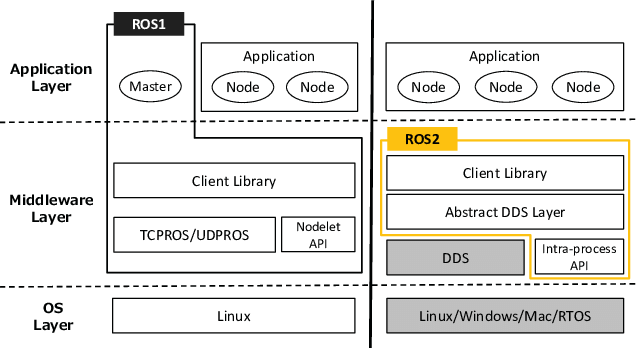
\includegraphics[width=0.99\textheight]{img/ros2/ROS1-ROS2-architecture-1.png}
        \caption{ROS 2 Architecture based on DDS}
    \end{figure}
\end{frame}

\begin{frame}[allowframebreaks]{What is DDS?}
    \begin{block}{Definition}
        \textbf{DDS (Data Distribution Service)} is an industry-standard protocol for real-time, scalable, and high-performance data exchange.
        \begin{itemize}
            \item Standardized by \textbf{Object Management Group (OMG)}
            \item Publish-subscribe middleware for distributed systems
            \item Used in mission-critical applications (aerospace, defense, healthcare)
        \end{itemize}
    \end{block}

    \framebreak

    \begin{block}{Key Features of DDS}
        \begin{itemize}
            \item \textbf{Decentralized}: No central broker required (peer-to-peer)
            \item \textbf{Quality of Service (QoS)}: Fine-grained control over reliability, latency, bandwidth
            \item \textbf{Data-centric}: Focus on data rather than connections
            \item \textbf{Discovery}: Automatic discovery of publishers and subscribers
            \item \textbf{Real-time capable}: Deterministic and low-latency communication
            \item \textbf{Scalable}: Supports large-scale distributed systems
        \end{itemize}
    \end{block}

    \framebreak

    \begin{block}{DDS Implementations in ROS 2}
        ROS 2 supports multiple DDS vendors:
        \begin{itemize}
            \item \textbf{Fast DDS} (eProsima): Default in ROS 2 Humble
            \item \textbf{Cyclone DDS} (Eclipse Foundation): Lightweight and fast
        \end{itemize}
    \end{block}

    \begin{alertblock}{Why DDS for ROS 2?}
        DDS solves ROS 1 limitations: no single point of failure, built-in QoS, real-time support, and production-ready reliability.
    \end{alertblock}
\end{frame}

\begin{frame}[allowframebreaks]{ROS 2 Distributions}
    \begin{block}{LTS (Long Term Support) Distributions}
        \begin{itemize}
            \item \textbf{Humble Hawksbill} (May 2022): Ubuntu 22.04, supported until May 2027
            \item \textbf{Foxy Fitzroy} (June 2020): Ubuntu 20.04, supported until May 2023
        \end{itemize}
    \end{block}

    \begin{block}{Current Distributions (as of 2024)}
        \begin{itemize}
            \item \textbf{Iron Irwini} (May 2023): Ubuntu 22.04
            \item \textbf{Jazzy Jalisco} (May 2024): Ubuntu 24.04
            \item Rolling Ridley: continuously updated development distribution
        \end{itemize}
    \end{block}

    \begin{alertblock}{Recommendation}
        For production and learning, use \textbf{Humble Hawksbill} (LTS version)
    \end{alertblock}
\end{frame}

\section{ROS 2 Concepts}

\begin{frame}[allowframebreaks]{ROS 2 Core Concepts}
    \begin{description}[leftmargin=3cm]
        \item[Nodes] Processes that perform computation. Same as ROS 1 but with improved lifecycle management.

        \item[Topics] Named buses for asynchronous communication using publish/subscribe pattern. Similar to ROS 1.

        \item[Services] Synchronous request-reply communication. Enhanced in ROS 2 with better timeout handling.

        \item[Actions] Asynchronous goal-oriented tasks with feedback. Improved implementation compared to ROS 1.

        \item[Parameters] Runtime configuration values for nodes. Enhanced with parameter events and better type safety.

        \item[Quality of Service (QoS)] NEW in ROS 2: fine-grained control over communication behavior (reliability, durability, etc.).
    \end{description}
\end{frame}

\begin{frame}{ROS 2 Communication: Topics}
    \begin{block}{Definition}
        Buses \textbf{many-to-many}, \textbf{asynchronous} communication using the publish-subscribe pattern.
        \begin{itemize}
            \item Multiple publishers/subscribers can send/receive messages to/from a topic
            \item Fire-and-forget: publishers don't wait for acknowledgment
            \item Best for: sensor data, continuous streams (e.g., camera images, laser scans)
        \end{itemize}
    \end{block}

    \begin{figure}
        \centering
        \href{https://docs.ros.org/en/foxy/Tutorials/Beginner-CLI-Tools/Understanding-ROS2-Topics/Understanding-ROS2-Topics.html}{%
            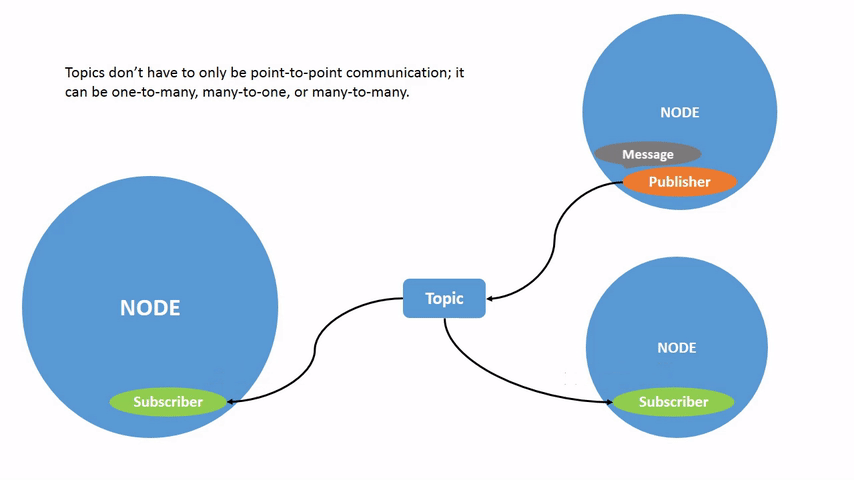
\includegraphics[width=0.5\textwidth]{img/ros2/ros2_communication.png}%
        }
        \caption{Topic communication pattern (click for tutorial)}
    \end{figure}
\end{frame}

\begin{frame}{ROS 2 Communication: Services}
    \begin{block}{Definition}
        Provide \textbf{one-to-one}, \textbf{synchronous} request-reply communication.
        \small
        \begin{itemize}
            \item Client sends a request and waits for response
            \item Server processes the request and sends back a reply
            \item Blocking operation: client waits for the response
            \item Best for: occasional tasks, computations (e.g., inverse kinematics, spawn entities)
        \end{itemize}
    \end{block}

    \begin{figure}
        \centering
        \href{https://docs.ros.org/en/foxy/Tutorials/Beginner-CLI-Tools/Understanding-ROS2-Services/Understanding-ROS2-Services.html}{%
            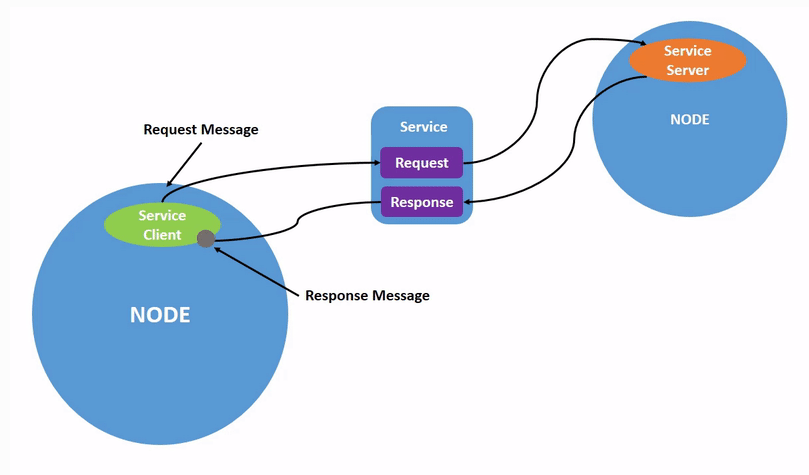
\includegraphics[width=0.5\textwidth]{img/ros2/ros2_communication_service.png}%
        }
        \caption{Service communication pattern (click for tutorial)}
    \end{figure}
\end{frame}

\begin{frame}{ROS 2 Communication: Actions}
    \begin{block}{Definition}
        Designed for \textbf{asynchronous}, \textbf{long-running} tasks with feedback and the ability to cancel.
        \begin{itemize}
            \item Client sends a goal and receives periodic feedback
            \item Server can send progress updates while executing
            \item Goals can be cancelled by the client
            \item Result is sent when the action completes
            \item Best for: navigation, manipulation, time-consuming operations
        \end{itemize}
    \end{block}

    \begin{figure}
        \centering
        \href{https://docs.ros.org/en/foxy/Tutorials/Beginner-CLI-Tools/Understanding-ROS2-Actions/Understanding-ROS2-Actions.html}{%
            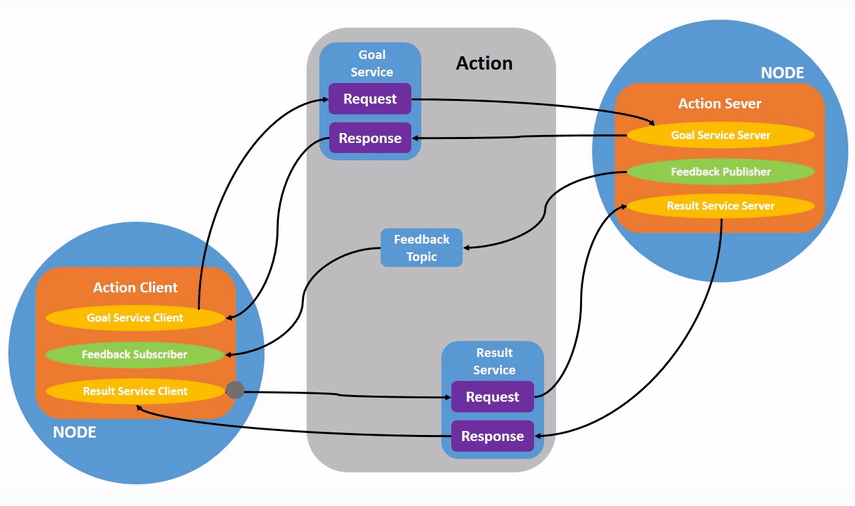
\includegraphics[width=0.3\textwidth]{img/ros2/ros2_communication_actions.png}%
        }
        \caption{Action communication pattern (click for tutorial)}
    \end{figure}
\end{frame}

\section{Installing ROS 2}

\begin{frame}[fragile, allowframebreaks]{Ubuntu install of ROS 2 Humble}
    ROS 2 Humble supports Ubuntu 22.04 (Jammy Jellyfish).

    \href{https://docs.ros.org/en/humble/Installation/Ubuntu-Install-Debs.html}{Installation instructions}

    \begin{enumerate}
        \item \textbf{Set locale}:
              \begin{lstlisting}[language=shell]
$ locale  # check for UTF-8
$ sudo apt update && sudo apt install locales
$ sudo locale-gen en_US en_US.UTF-8
$ sudo update-locale LC_ALL=en_US.UTF-8 LANG=en_US.UTF-8
$ export LANG=en_US.UTF-8
\end{lstlisting}

        \item \textbf{Setup Sources}:
              \begin{lstlisting}[language=shell]
$ sudo apt install software-properties-common
$ sudo add-apt-repository universe
$ sudo apt update && sudo apt install curl -y
$ sudo curl -sSL https://raw.githubusercontent.com/ros/rosdistro/master/ros.key -o /usr/share/keyrings/ros-archive-keyring.gpg
\end{lstlisting}

              \framebreak

              \begin{lstlisting}[language=shell]
$ echo "deb [arch=$(dpkg --print-architecture) signed-by=/usr/share/keyrings/ros-archive-keyring.gpg] http://packages.ros.org/ros2/ubuntu $(. /etc/os-release && echo $UBUNTU_CODENAME) main" | sudo tee /etc/apt/sources.list.d/ros2.list > /dev/null
\end{lstlisting}

        \item \textbf{Install ROS 2 packages}:
              \begin{lstlisting}[language=shell]
$ sudo apt update
$ sudo apt upgrade
$ sudo apt install ros-humble-desktop
\end{lstlisting}

        \item \textbf{Environment setup}:
              \begin{lstlisting}[language=shell]
$ source /opt/ros/humble/setup.bash
$ echo "source /opt/ros/humble/setup.bash" >> ~/.bashrc
\end{lstlisting}

        \item \textbf{Install development tools}:
              \begin{lstlisting}[language=shell]
$ sudo apt install ros-dev-tools
\end{lstlisting}
    \end{enumerate}
\end{frame}

\begin{frame}[fragile, allowframebreaks]{Setting up Docker image for ROS 2}
    \begin{enumerate}
        \item \textbf{Download the image from Docker Hub}:
              \begin{lstlisting}[language=shell]
$ docker pull osrf/ros:humble-desktop-full
\end{lstlisting}

        \item \textbf{Launch the container using Rocker}:
              \begin{lstlisting}[language=shell]
$ rocker --nvidia --x11 --network host --name ros2-humble --volume <path_to_shared_folder>:/root/ros2_ws -- docker.io/osrf/ros:humble-desktop-full
\end{lstlisting}
              \textcolor{blue}{- -nvidia option only if the computer has a graphic card}\\
              \textcolor{blue}{- -volume for sharing folder between host and container}

        \item \textbf{To open a new terminal inside the container}:
              \begin{lstlisting}[language=shell]
$ docker exec -it ros2-humble /bin/bash 
\end{lstlisting}

              \framebreak

        \item \textbf{To source the ROS 2 environment}:
              \begin{lstlisting}[language=shell]
$ source /opt/ros/humble/setup.bash
\end{lstlisting}

        \item \textbf{To source the workspace} (after building):
              \begin{lstlisting}[language=shell]
$ source /root/ros2_ws/install/setup.bash
\end{lstlisting}
    \end{enumerate}
\end{frame}

\begin{frame}[fragile]{Verify Installation}
    Test that ROS 2 is installed correctly:

    \begin{lstlisting}[language=shell]
$ ros2 --help
\end{lstlisting}

    You should see a list of available commands:
    \begin{lstlisting}[language=output]
usage: ros2 [-h] Call `ros2 <command> -h` for more detailed usage. ...

ros2 is an extensible command-line tool for ROS 2.
  ...
\end{lstlisting}

    \framebreak

    Main commands:
    \begin{lstlisting}[language=syntax]
ros2 node      # Node introspection tools
ros2 topic     # Topic introspection tools
ros2 service   # Service introspection tools
ros2 action    # Action introspection tools
ros2 param     # Parameter introspection tools
ros2 bag       # Recording and playback tools
ros2 run       # Run a node
ros2 launch    # Launch files
ros2 pkg       # Package tools
ros2 interface # Interface introspection
\end{lstlisting}
\end{frame}

\section{ROS 2 Workspace}

\begin{frame}[fragile, allowframebreaks]{Creating a ROS 2 Workspace}
    A ROS 2 workspace is organized differently from ROS 1:

    \begin{lstlisting}[language=shell]
$ mkdir -p ~/ros2_ws/src
$ cd ~/ros2_ws
\end{lstlisting}

    \textbf{Build the workspace} using colcon (Inside the ros2\_ws directory):
    \begin{lstlisting}[language=shell]
$ colcon build
\end{lstlisting}

    After building, you'll have these directories:
    \begin{lstlisting}[language=syntax]
ros2_ws/
  build/    # Build artifacts
  install/  # Installation files
  log/      # Build logs
  src/      # Source code
\end{lstlisting}

    \framebreak

    \textbf{Source the workspace}:
    \begin{lstlisting}[language=shell]
$ source ~/ros2_ws/install/setup.bash
\end{lstlisting}

    To automatically source on every new terminal:
    \begin{lstlisting}[language=shell]
$ echo "source ~/ros2_ws/install/setup.bash" >> ~/.bashrc
\end{lstlisting}

    \begin{alertblock}{Build specific packages}
        \begin{lstlisting}[language=shell]
$ colcon build --packages-select <package_name>
\end{lstlisting}
    \end{alertblock}
\end{frame}

\begin{frame}[fragile]{Installing Turtlesim}
    \textbf{Turtlesim} is a lightweight simulator for learning ROS 2 concepts.
    \\ \href{https://docs.ros.org/en/humble/Tutorials/Beginner-CLI-Tools/Introducing-Turtlesim/Introducing-Turtlesim.html}{Learn more about Turtlesim.}

    \begin{block}{Install on Ubuntu}
        \begin{lstlisting}[language=shell]
$ sudo apt update
$ sudo apt install ros-humble-turtlesim
\end{lstlisting}
    \end{block}

    \begin{block}{Verify installation}
        Check if turtlesim package is available:
        \begin{lstlisting}[language=shell]
$ ros2 pkg executables turtlesim
turtlesim draw_square
turtlesim mimic
turtlesim turtle_teleop_key
turtlesim turtlesim_node
\end{lstlisting}
    \end{block}
\end{frame}

\begin{frame}[fragile]{Running Turtlesim}
    \textbf{Start the turtlesim node}:
    \begin{lstlisting}[language=shell]
$ ros2 run turtlesim turtlesim_node
\end{lstlisting}

    A window will appear with a turtle in the center.

    \vspace{0.5cm}

    \textbf{In a new terminal, start the teleop node}:
    \begin{lstlisting}[language=shell]
$ ros2 run turtlesim turtle_teleop_key
\end{lstlisting}

    Use arrow keys to control the turtle!

    \begin{alertblock}{Tip}
        Make sure the terminal with \texttt{turtle\_teleop\_key} is active (in focus) when pressing arrow keys.
    \end{alertblock}
\end{frame}

\begin{frame}[fragile]{Turtlesim in Docker}
    If running ROS 2 in Docker, you need X11 forwarding for GUI applications.

    \begin{block}{Using Rocker (recommended)}
        \begin{lstlisting}[language=shell]
$ rocker --x11 --nvidia osrf/ros:humble-desktop-full
\end{lstlisting}
    \end{block}

    \begin{block}{Inside the container}
        \begin{lstlisting}[language=shell]
$ source /opt/ros/humble/setup.bash
$ apt update && apt install -y ros-humble-turtlesim
$ ros2 run turtlesim turtlesim_node
\end{lstlisting}
    \end{block}

    \begin{alertblock}{Note}
        The \texttt{--x11} flag enables X11 forwarding for displaying GUI windows.
    \end{alertblock}
\end{frame}

\begin{frame}[fragile, allowframebreaks]{Working with Nodes}
    \textbf{List running nodes}:
    \begin{lstlisting}[language=shell]
$ ros2 node list
\end{lstlisting}

    \textbf{Get node information}:
    \begin{lstlisting}[language=shell]
$ ros2 node info /node_name
\end{lstlisting}

    \textbf{Run a node}:
    \begin{lstlisting}[language=shell]
$ ros2 run <package_name> <executable_name>
\end{lstlisting}

    Example with turtlesim:
    \begin{lstlisting}[language=shell]
$ sudo apt install ros-humble-turtlesim
$ ros2 run turtlesim turtlesim_node
\end{lstlisting}

    \framebreak

    \textbf{Remap node name}:
    \begin{lstlisting}[language=shell]
$ ros2 run turtlesim turtlesim_node --ros-args --remap __node:=my_turtle
\end{lstlisting}

    \textbf{Get node info}:
    \begin{lstlisting}[language=shell]
$ ros2 node info /turtlesim
Node [/turtlesim]
  Subscribers:
    /turtle1/cmd_vel: geometry_msgs/msg/Twist
  Publishers:
    /turtle1/color_sensor: turtlesim/msg/Color
    /turtle1/pose: turtlesim/msg/Pose
  Service Servers:
    /clear: std_srvs/srv/Empty
    /kill: turtlesim/srv/Kill
    ...
\end{lstlisting}
\end{frame}

\begin{frame}[fragile, allowframebreaks]{Working with Topics}
    \textbf{List topics}:
    \begin{lstlisting}[language=shell]
$ ros2 topic list
$ ros2 topic list -t  # Show message types
\end{lstlisting}

    \textbf{Echo topic messages}:
    \begin{lstlisting}[language=shell]
$ ros2 topic echo /turtle1/cmd_vel
\end{lstlisting}

    \textbf{Get topic info}:
    \begin{lstlisting}[language=shell]
$ ros2 topic info /turtle1/cmd_vel
Type: geometry_msgs/msg/Twist
Publisher count: 1
Subscription count: 1
\end{lstlisting}

    \framebreak

    \textbf{Publish to a topic}:
    \begin{lstlisting}[language=shell]
$ ros2 topic pub /turtle1/cmd_vel geometry_msgs/msg/Twist "{linear: {x: 2.0, y: 0.0, z: 0.0}, angular: {x: 0.0, y: 0.0, z: 1.8}}"
\end{lstlisting}

    Add \texttt{--once} to publish once or \texttt{--rate 1} for continuous publishing at 1 Hz.

    \textbf{Get publishing frequency}:
    \begin{lstlisting}[language=shell]
$ ros2 topic hz /turtle1/pose
average rate: 62.506
	min: 0.014s max: 0.018s std dev: 0.00070s window: 64
\end{lstlisting}

    \textbf{Get bandwidth}:
    \begin{lstlisting}[language=shell]
$ ros2 topic bw /turtle1/pose
\end{lstlisting}
\end{frame}

\begin{frame}[fragile, allowframebreaks]{Working with Services}
    \textbf{List services}:
    \begin{lstlisting}[language=shell]
$ ros2 service list
$ ros2 service list -t  # Show service types
\end{lstlisting}

    \textbf{Get service type}:
    \begin{lstlisting}[language=shell]
$ ros2 service type /clear
std_srvs/srv/Empty
\end{lstlisting}

    \textbf{Find services by type}:
    \begin{lstlisting}[language=shell]
$ ros2 service find std_srvs/srv/Empty
/clear
/reset
\end{lstlisting}

    \framebreak

    \textbf{Call a service}:
    \begin{lstlisting}[language=shell]
$ ros2 service call /clear std_srvs/srv/Empty
\end{lstlisting}

    Spawn a new turtle:
    \begin{lstlisting}[language=shell]
$ ros2 service call /spawn turtlesim/srv/Spawn "{x: 2.0, y: 2.0, theta: 0.2, name: 'turtle2'}"
\end{lstlisting}

    \textbf{Show service interface}:
    \begin{lstlisting}[language=shell]
$ ros2 interface show turtlesim/srv/Spawn
float32 x
float32 y
float32 theta
string name
---
string name
\end{lstlisting}
\end{frame}

\begin{frame}[fragile, allowframebreaks]{Working with Parameters}
    \textbf{List parameters}:
    \begin{lstlisting}[language=shell]
$ ros2 param list
\end{lstlisting}

    \textbf{Get parameter value}:
    \begin{lstlisting}[language=shell]
$ ros2 param get /turtlesim background_r
Integer value is: 69
\end{lstlisting}

    \textbf{Set parameter value}:
    \begin{lstlisting}[language=shell]
$ ros2 param set /turtlesim background_r 150
Set parameter successful
\end{lstlisting}

    \framebreak

    \textbf{Dump parameters to file}:
    \begin{lstlisting}[language=shell]
$ ros2 param dump /turtlesim
Saving to:  ./turtlesim.yaml
\end{lstlisting}

    \textbf{Load parameters from file}:
    \begin{lstlisting}[language=shell]
$ ros2 param load /turtlesim turtlesim.yaml
\end{lstlisting}

    \textbf{Start node with parameters}:
    \begin{lstlisting}[language=shell]
$ ros2 run turtlesim turtlesim_node --ros-args --params-file turtlesim.yaml
\end{lstlisting}
\end{frame}

\begin{frame}[fragile, allowframebreaks]{Working with Actions}
    Actions are for long-running tasks with feedback.

    \textbf{List actions}:
    \begin{lstlisting}[language=shell]
$ ros2 action list
$ ros2 action list -t  # Show action types
\end{lstlisting}

    \textbf{Get action info}:
    \begin{lstlisting}[language=shell]
$ ros2 action info /turtle1/rotate_absolute
Action: /turtle1/rotate_absolute
Action clients: 0
Action servers: 1
    /turtlesim
\end{lstlisting}

    \framebreak

    \textbf{Show action interface}:
    \begin{lstlisting}[language=shell]
$ ros2 interface show turtlesim/action/RotateAbsolute
# Goal
float32 theta
---
# Result
float32 delta
---
# Feedback
float32 remaining
\end{lstlisting}

    \textbf{Send action goal}:
    \begin{lstlisting}[language=shell]
$ ros2 action send_goal /turtle1/rotate_absolute turtlesim/action/RotateAbsolute "{theta: 1.57}" --feedback
\end{lstlisting}
\end{frame}

\section{Creating ROS 2 Packages}

\begin{frame}[fragile, allowframebreaks]{Creating a Package}
    ROS 2 supports two build types: \textbf{ament\_cmake} and \textbf{ament\_python}.

    \textbf{Create a Python package}:
    \begin{lstlisting}[language=shell]
$ cd ~/ros2_ws/src
$ ros2 pkg create --build-type ament_python --node-name my_node my_package
\end{lstlisting}

    \textbf{Create a C++ package}:
    \begin{lstlisting}[language=shell]
$ ros2 pkg create --build-type ament_cmake --node-name my_node my_package --dependencies rclcpp std_msgs
\end{lstlisting}

    \framebreak

    \textbf{Package structure} (Python):
    \begin{lstlisting}[language=syntax]
my_package/
  my_package/
    __init__.py
    my_node.py
  resource/
    my_package
  test/
  package.xml
  setup.py
  setup.cfg
\end{lstlisting}

    \framebreak

    \textbf{Package structure} (C++):
    \begin{lstlisting}[language=syntax]
my_package/
  include/
    my_package/
  src/
    my_node.cpp
  CMakeLists.txt
  package.xml
\end{lstlisting}
\end{frame}

\begin{frame}[fragile]{Building and Running}
    \textbf{Build the package}:
    \begin{lstlisting}[language=shell]
$ cd ~/ros2_ws
$ colcon build --packages-select my_package
\end{lstlisting}

    \textbf{Source the workspace}:
    \begin{lstlisting}[language=shell]
$ source ~/ros2_ws/install/setup.bash
\end{lstlisting}

    \textbf{Run the node}:
    \begin{lstlisting}[language=shell]
$ ros2 run my_package my_node
\end{lstlisting}

    \begin{alertblock}{Tip}
        Use \texttt{--symlink-install} flag for Python packages to avoid rebuilding after code changes:
        \begin{lstlisting}[language=shell]
$ colcon build --symlink-install
\end{lstlisting}
    \end{alertblock}
\end{frame}

\section{Writing Nodes in Python}

\begin{frame}[fragile, allowframebreaks]{Simple Publisher (Python)}
    Create file \texttt{publisher\_member\_function.py}:

    \begin{lstlisting}[language=python]
import rclpy
from rclpy.node import Node
from std_msgs.msg import String

class MinimalPublisher(Node):
    def __init__(self):
        super().__init__('minimal_publisher')
        self.publisher_ = self.create_publisher(String, 'topic', 10)
        timer_period = 0.5  # seconds
        self.timer = self.create_timer(timer_period, self.timer_callback)
        self.i = 0

    def timer_callback(self):
        msg = String()
        msg.data = 'Hello World: %d' % self.i
        self.publisher_.publish(msg)
        self.get_logger().info('Publishing: "%s"' % msg.data)
        self.i += 1

def main(args=None):
    rclpy.init(args=args)
    minimal_publisher = MinimalPublisher()
    rclpy.spin(minimal_publisher)
    minimal_publisher.destroy_node()
    rclpy.shutdown()

if __name__ == '__main__':
    main()
\end{lstlisting}

    \framebreak

    \textbf{Key concepts}:
    \begin{itemize}
        \item \texttt{rclpy.init()}: Initialize ROS 2 Python client library
        \item \texttt{Node}: Base class for ROS 2 nodes
        \item \texttt{create\_publisher()}: Create a publisher with topic name, message type, and QoS
        \item \texttt{create\_timer()}: Create a timer for periodic callbacks
        \item \texttt{rclpy.spin()}: Keep the node running
        \item \texttt{get\_logger()}: Built-in logging functionality
    \end{itemize}
\end{frame}

\begin{frame}[fragile, allowframebreaks]{Simple Subscriber (Python)}
    Create file \texttt{subscriber\_member\_function.py}:

    \begin{lstlisting}[language=python]
import rclpy
from rclpy.node import Node
from std_msgs.msg import String

class MinimalSubscriber(Node):
    def __init__(self):
        super().__init__('minimal_subscriber')
        self.subscription = self.create_subscription(
            String,
            'topic',
            self.listener_callback,
            10)
        self.subscription  # prevent unused variable warning

    def listener_callback(self, msg):
        self.get_logger().info('I heard: "%s"' % msg.data)

def main(args=None):
    rclpy.init(args=args)
    minimal_subscriber = MinimalSubscriber()
    rclpy.spin(minimal_subscriber)
    minimal_subscriber.destroy_node()
    rclpy.shutdown()

if __name__ == '__main__':
    main()
\end{lstlisting}

    \framebreak

    \textbf{Add to setup.py}:
    \begin{lstlisting}[language=python]
entry_points={
    'console_scripts': [
        'talker = my_package.publisher_member_function:main',
        'listener = my_package.subscriber_member_function:main',
    ],
},
\end{lstlisting}

    \textbf{Build and run}:
    \begin{lstlisting}[language=shell]
$ cd ~/ros2_ws
$ colcon build --packages-select my_package
$ source install/setup.bash
$ ros2 run my_package talker
\end{lstlisting}

    In another terminal:
    \begin{lstlisting}[language=shell]
$ ros2 run my_package listener
\end{lstlisting}
\end{frame}

\begin{frame}[fragile, allowframebreaks]{Service Server (Python)}
    Create file \texttt{service\_member\_function.py}:

    \begin{lstlisting}[language=python]
from example_interfaces.srv import AddTwoInts
import rclpy
from rclpy.node import Node

class MinimalService(Node):
    def __init__(self):
        super().__init__('minimal_service')
        self.srv = self.create_service(
            AddTwoInts, 
            'add_two_ints', 
            self.add_two_ints_callback)

    def add_two_ints_callback(self, request, response):
        response.sum = request.a + request.b
        self.get_logger().info(
            'Incoming request\na: %d b: %d' % (request.a, request.b))
        return response

def main(args=None):
    rclpy.init(args=args)
    minimal_service = MinimalService()
    rclpy.spin(minimal_service)
    rclpy.shutdown()

if __name__ == '__main__':
    main()
\end{lstlisting}
\end{frame}

\begin{frame}[fragile, allowframebreaks]{Service Client (Python)}
    Create file \texttt{client\_member\_function.py}:

    \begin{lstlisting}[language=python]
import sys
from example_interfaces.srv import AddTwoInts
import rclpy
from rclpy.node import Node

class MinimalClientAsync(Node):
    def __init__(self):
        super().__init__('minimal_client_async')
        self.cli = self.create_client(AddTwoInts, 'add_two_ints')
        while not self.cli.wait_for_service(timeout_sec=1.0):
            self.get_logger().info('service not available, waiting...')
        self.req = AddTwoInts.Request()

    def send_request(self, a, b):
        self.req.a = a
        self.req.b = b
        self.future = self.cli.call_async(self.req)
        rclpy.spin_until_future_complete(self, self.future)
        return self.future.result()

def main(args=None):
    rclpy.init(args=args)
    minimal_client = MinimalClientAsync()
    response = minimal_client.send_request(int(sys.argv[1]), int(sys.argv[2]))
    minimal_client.get_logger().info(
        'Result of add_two_ints: %d + %d = %d' %
        (int(sys.argv[1]), int(sys.argv[2]), response.sum))
    minimal_client.destroy_node()
    rclpy.shutdown()

if __name__ == '__main__':
    main()
\end{lstlisting}
\end{frame}

\section{Launch Files}

\begin{frame}[fragile, allowframebreaks]{ROS 2 Launch Files}
    Launch files in ROS 2 can be written in \textbf{Python}, XML, or YAML.

    \textbf{Python launch file} (\texttt{my\_launch.py}):
    \begin{lstlisting}[language=python]
from launch import LaunchDescription
from launch_ros.actions import Node

def generate_launch_description():
    return LaunchDescription([
        Node(
            package='turtlesim',
            executable='turtlesim_node',
            name='sim'
        ),
        Node(
            package='turtlesim',
            executable='turtle_teleop_key',
            name='teleop',
            prefix='xterm -e',
            output='screen'
        ),
    ])
\end{lstlisting}

    \framebreak

    \textbf{Create launch directory}:
    \begin{lstlisting}[language=shell]
$ mkdir -p ~/ros2_ws/src/my_package/launch
\end{lstlisting}

    \textbf{Update setup.py} to include launch files:
    \begin{lstlisting}[language=python]
import os
from glob import glob
# ...

data_files=[
    # ...
    (os.path.join('share', package_name, 'launch'), 
     glob('launch/*.py')),
],
\end{lstlisting}

    \framebreak

    \textbf{Run launch file}:
    \begin{lstlisting}[language=shell]
$ ros2 launch my_package my_launch.py
\end{lstlisting}

    \textbf{Launch with arguments}:
    \begin{lstlisting}[language=python]
from launch.actions import DeclareLaunchArgument
from launch.substitutions import LaunchConfiguration

def generate_launch_description():
    return LaunchDescription([
        DeclareLaunchArgument('use_sim_time', default_value='false'),
        Node(
            package='my_package',
            executable='my_node',
            parameters=[{'use_sim_time': LaunchConfiguration('use_sim_time')}]
        ),
    ])
\end{lstlisting}

    \begin{lstlisting}[language=shell]
$ ros2 launch my_package my_launch.py use_sim_time:=true
\end{lstlisting}
\end{frame}

\section{Custom Interfaces}

\begin{frame}[fragile, allowframebreaks]{Creating Custom Messages}
    \textbf{Create interface package}:
    \begin{lstlisting}[language=shell]
$ ros2 pkg create --build-type ament_cmake tutorial_interfaces
\end{lstlisting}

    \textbf{Create directory structure}:
    \begin{lstlisting}[language=shell]
$ mkdir -p tutorial_interfaces/msg
$ mkdir -p tutorial_interfaces/srv
$ mkdir -p tutorial_interfaces/action
\end{lstlisting}

    \textbf{Create custom message} (\texttt{msg/Num.msg}):
    \begin{lstlisting}[language=syntax]
int64 num
\end{lstlisting}

    \textbf{Create custom message with nested types} (\texttt{msg/Sphere.msg}):
    \begin{lstlisting}[language=syntax]
geometry_msgs/Point center
float64 radius
\end{lstlisting}

    \framebreak

    \textbf{Update CMakeLists.txt}:
    \begin{lstlisting}[language=syntax]
find_package(geometry_msgs REQUIRED)
find_package(rosidl_default_generators REQUIRED)

rosidl_generate_interfaces(${PROJECT_NAME}
  "msg/Num.msg"
  "msg/Sphere.msg"
  DEPENDENCIES geometry_msgs
)
\end{lstlisting}

    \textbf{Update package.xml}:
    \begin{lstlisting}[language=xml]
<depend>geometry_msgs</depend>
<buildtool_depend>rosidl_default_generators</buildtool_depend>
<exec_depend>rosidl_default_runtime</exec_depend>
<member_of_group>rosidl_interface_packages</member_of_group>
\end{lstlisting}

    \framebreak

    \textbf{Build the interface package}:
    \begin{lstlisting}[language=shell]
$ cd ~/ros2_ws
$ colcon build --packages-select tutorial_interfaces
$ source install/setup.bash
\end{lstlisting}

    \textbf{Verify the interface}:
    \begin{lstlisting}[language=shell]
$ ros2 interface show tutorial_interfaces/msg/Num
int64 num
\end{lstlisting}

    \textbf{Use in your node}:
    \begin{lstlisting}[language=python]
from tutorial_interfaces.msg import Num

# In your node:
self.publisher_ = self.create_publisher(Num, 'topic', 10)
msg = Num()
msg.num = 42
\end{lstlisting}
\end{frame}

\begin{frame}[fragile, allowframebreaks]{Creating Custom Services}
    \textbf{Create service definition} (\texttt{srv/AddThreeInts.srv}):
    \begin{lstlisting}[language=syntax]
int64 a
int64 b
int64 c
---
int64 sum
\end{lstlisting}

    \textbf{Update CMakeLists.txt}:
    \begin{lstlisting}[language=syntax]
rosidl_generate_interfaces(${PROJECT_NAME}
  "msg/Num.msg"
  "srv/AddThreeInts.srv"
)
\end{lstlisting}

    Build and verify:
    \begin{lstlisting}[language=shell]
$ colcon build --packages-select tutorial_interfaces
$ ros2 interface show tutorial_interfaces/srv/AddThreeInts
\end{lstlisting}
\end{frame}


\begin{frame}[allowframebreaks]{Quality of Service (QoS)}
    \begin{block}{What is QoS?}
        Quality of Service policies allow you to configure the behavior of communication in ROS 2:
        \begin{itemize}
            \item \textbf{Reliability}: Reliable (guaranteed delivery) vs Best Effort
            \item \textbf{Durability}: Transient Local (late joiners get last message) vs Volatile
            \item \textbf{History}: Keep Last N messages vs Keep All
            \item \textbf{Deadline}: Maximum time between messages
            \item \textbf{Lifespan}: Maximum age of a message
        \end{itemize}
    \end{block}

    \framebreak

    \begin{block}{QoS Profiles}
        ROS 2 provides predefined QoS profiles:
        \begin{itemize}
            \item \textbf{Sensor Data}: Best effort, volatile (e.g., camera images)
            \item \textbf{Parameters}: Reliable, volatile (e.g., configuration)
            \item \textbf{Services}: Reliable, volatile
            \item \textbf{System Default}: Reliable, volatile, keep last 10
        \end{itemize}
    \end{block}

    \begin{alertblock}{Important}
        Publishers and subscribers must have \textbf{compatible} QoS policies to communicate!
    \end{alertblock}
\end{frame}

\section{ROS 2 Tools and Visualization}

\begin{frame}[fragile, allowframebreaks]{ROS 2 Bag}
    \textbf{rosbag2} is used for recording and playing back topic data.

    \textbf{Record topics}:
    \begin{lstlisting}[language=shell]
$ ros2 bag record /turtle1/cmd_vel /turtle1/pose
\end{lstlisting}

    \textbf{Record all topics}:
    \begin{lstlisting}[language=shell]
$ ros2 bag record -a
\end{lstlisting}

    \textbf{Record with output name}:
    \begin{lstlisting}[language=shell]
$ ros2 bag record -o my_bag /topic1 /topic2
\end{lstlisting}

    \framebreak

    \textbf{Get bag info}:
    \begin{lstlisting}[language=shell]
$ ros2 bag info my_bag
\end{lstlisting}

    \textbf{Play bag}:
    \begin{lstlisting}[language=shell]
$ ros2 bag play my_bag
\end{lstlisting}

    \textbf{Play at different rate}:
    \begin{lstlisting}[language=shell]
$ ros2 bag play my_bag --rate 2.0  # 2x speed
\end{lstlisting}

    \textbf{Play in loop}:
    \begin{lstlisting}[language=shell]
$ ros2 bag play my_bag --loop
\end{lstlisting}
\end{frame}

\begin{frame}[fragile]{RQT and Visualization Tools}
    \textbf{rqt} is a Qt-based framework for GUI development in ROS 2.

    \textbf{Launch rqt}:
    \begin{lstlisting}[language=shell]
$ rqt
\end{lstlisting}

    \textbf{Useful rqt plugins}:
    \begin{itemize}
        \item \texttt{rqt\_graph}: Visualize node graph
        \item \texttt{rqt\_console}: View log messages
        \item \texttt{rqt\_plot}: Plot topic data
        \item \texttt{rqt\_publisher}: Publish messages
        \item \texttt{rqt\_service\_caller}: Call services
        \item \texttt{rqt\_reconfigure}: Dynamic reconfigure (limited in ROS 2)
    \end{itemize}

    \begin{lstlisting}[language=shell]
$ ros2 run rqt_graph rqt_graph
$ ros2 run rqt_console rqt_console
$ ros2 run rqt_plot rqt_plot
\end{lstlisting}
\end{frame}



% \begin{frame}[fragile]{TF2 - Transform Library}
%     \textbf{TF2} tracks coordinate frames over time.

%     \textbf{View TF tree}:
%     \begin{lstlisting}[language=shell]
% $ ros2 run tf2_tools view_frames
% \end{lstlisting}

%     \textbf{Echo transform}:
%     \begin{lstlisting}[language=shell]
% $ ros2 run tf2_ros tf2_echo [source_frame] [target_frame]
% \end{lstlisting}

%     \textbf{Static transform publisher}:
%     \begin{lstlisting}[language=shell]
% $ ros2 run tf2_ros static_transform_publisher x y z yaw pitch roll parent_frame child_frame
% \end{lstlisting}

%     Example:
%     \begin{lstlisting}[language=shell]
% $ ros2 run tf2_ros static_transform_publisher 0 0 1 0 0 0 base_link camera_link
% \end{lstlisting}
% \end{frame}

% \section{Advanced Topics}

% \begin{frame}[fragile, allowframebreaks]{Lifecycle Nodes}
%     ROS 2 introduces \textbf{managed nodes} with defined lifecycle states:

%     %\begin{figure}
%     %    \centering
%     %    \includegraphics[width=0.7\textwidth]{img/lifecycle.png}
%     %    \caption{Lifecycle node states}
%     %\end{figure}

%     \textbf{States}:
%     \begin{itemize}
%         \item \textbf{Unconfigured}: Initial state
%         \item \textbf{Inactive}: Configured but not active
%         \item \textbf{Active}: Fully operational
%         \item \textbf{Finalized}: Shutdown
%     \end{itemize}

%     \framebreak

%     \textbf{Transitions}:
%     \begin{itemize}
%         \item \texttt{configure}: Unconfigured → Inactive
%         \item \texttt{activate}: Inactive → Active
%         \item \texttt{deactivate}: Active → Inactive
%         \item \texttt{cleanup}: Inactive → Unconfigured
%         \item \texttt{shutdown}: Any state → Finalized
%     \end{itemize}

%     \textbf{Control lifecycle node}:
%     \begin{lstlisting}[language=shell]
% $ ros2 lifecycle set /node_name configure
% $ ros2 lifecycle set /node_name activate
% $ ros2 lifecycle get /node_name
% \end{lstlisting}
% \end{frame}

% \begin{frame}[fragile, allowframebreaks]{Executors and Callbacks}
%     ROS 2 provides different \textbf{executor} types for handling callbacks:

%     \begin{itemize}
%         \item \textbf{SingleThreadedExecutor}: Default, single thread
%         \item \textbf{MultiThreadedExecutor}: Multiple threads
%         \item \textbf{StaticSingleThreadedExecutor}: Optimized single thread
%     \end{itemize}

%     \textbf{Using MultiThreadedExecutor}:
%     \begin{lstlisting}[language=python]
% import rclpy
% from rclpy.executors import MultiThreadedExecutor

% rclpy.init()
% node1 = MyNode1()
% node2 = MyNode2()

% executor = MultiThreadedExecutor()
% executor.add_node(node1)
% executor.add_node(node2)

% try:
%     executor.spin()
% finally:
%     executor.shutdown()
%     node1.destroy_node()
%     node2.destroy_node()
%     rclpy.shutdown()
% \end{lstlisting}

%     \framebreak

%     \textbf{Callback groups}:
%     \begin{lstlisting}[language=python]
% from rclpy.callback_groups import ReentrantCallbackGroup, MutuallyExclusiveCallbackGroup

% class MyNode(Node):
%     def __init__(self):
%         super().__init__('my_node')

%         # Callbacks in this group can execute in parallel
%         self.reentrant_group = ReentrantCallbackGroup()

%         # Callbacks in this group execute sequentially
%         self.exclusive_group = MutuallyExclusiveCallbackGroup()

%         self.timer1 = self.create_timer(
%             1.0, self.callback1, callback_group=self.reentrant_group)
%         self.timer2 = self.create_timer(
%             1.0, self.callback2, callback_group=self.exclusive_group)
% \end{lstlisting}
% \end{frame}

% \begin{frame}[fragile, allowframebreaks]{Composition}
%     ROS 2 supports \textbf{composable nodes} - multiple nodes in a single process.

%     \textbf{Benefits}:
%     \begin{itemize}
%         \item Reduced overhead (no inter-process communication)
%         \item Better performance
%         \item Shared memory communication
%     \end{itemize}

%     \textbf{Create composable node}:
%     \begin{lstlisting}[language=python]
% import rclpy
% from rclpy.node import Node

% class MyComposableNode(Node):
%     def __init__(self, options=None):
%         super().__init__('my_composable_node', 
%                          allow_undeclared_parameters=True,
%                          automatically_declare_parameters_from_overrides=True)
%         # Node implementation...

% def main(args=None):
%     rclpy.init(args=args)
%     node = MyComposableNode()
%     rclpy.spin(node)
%     rclpy.shutdown()
% \end{lstlisting}

%     \framebreak

%     \textbf{Launch composed nodes}:
%     \begin{lstlisting}[language=python]
% from launch import LaunchDescription
% from launch_ros.actions import ComposableNodeContainer
% from launch_ros.descriptions import ComposableNode

% def generate_launch_description():
%     container = ComposableNodeContainer(
%         name='my_container',
%         namespace='',
%         package='rclcpp_components',
%         executable='component_container',
%         composable_node_descriptions=[
%             ComposableNode(
%                 package='my_package',
%                 plugin='my_package::MyNode1',
%                 name='node1'),
%             ComposableNode(
%                 package='my_package',
%                 plugin='my_package::MyNode2',
%                 name='node2'),
%         ],
%         output='screen',
%     )
%     return LaunchDescription([container])
% \end{lstlisting}
% \end{frame}

\section{Best Practices}

\begin{frame}{ROS 2 Best Practices}
    \begin{enumerate}
        \item \textbf{Use appropriate QoS profiles} for your application
              \begin{itemize}
                  \item Sensor data: Best effort
                  \item Commands: Reliable
                  \item State: Transient local
              \end{itemize}

        \item \textbf{Namespace your nodes} to avoid conflicts

        \item \textbf{Use parameters} for configuration, not hardcoded values

        \item \textbf{Log appropriately}: DEBUG, INFO, WARN, ERROR, FATAL

        \item \textbf{Handle shutdown gracefully}: cleanup resources

        \item \textbf{Use lifecycle nodes} for critical systems

        \item \textbf{Write launch files} instead of manual node starting

        \item \textbf{Use composition} for performance-critical applications
    \end{enumerate}
\end{frame}

\begin{frame}[fragile]{Package Organization}
    \textbf{Good package structure}:
    \begin{lstlisting}[language=syntax]
my_robot/
  my_robot_bringup/        # Launch files
  my_robot_description/    # URDF/meshes
  my_robot_control/        # Control nodes
  my_robot_navigation/     # Navigation configuration
  my_robot_interfaces/     # Custom messages/services
  my_robot_gazebo/        # Simulation
\end{lstlisting}

    \textbf{Principles}:
    \begin{itemize}
        \item One package = one clear purpose
        \item Separate interfaces from implementation
        \item Keep launch files in dedicated packages
        \item Use package dependencies appropriately
    \end{itemize}
\end{frame}

\begin{frame}{Migration from ROS 1 to ROS 2}
    \begin{block}{Key Differences}
        \begin{itemize}
            \item No \texttt{roscore} required
            \item \texttt{colcon} instead of \texttt{catkin\_make}
            \item Different build types: \texttt{ament\_cmake}, \texttt{ament\_python}
            \item \texttt{ros2} CLI instead of separate tools
            \item Different client libraries APIs
            \item QoS policies
            \item Launch files in Python (preferred)
            \item Different parameter handling
        \end{itemize}
    \end{block}

    \begin{alertblock}{Tools}
        \texttt{ros1\_bridge} allows ROS 1 and ROS 2 nodes to communicate
    \end{alertblock}
\end{frame}

\section{Practical Exercise}

\begin{frame}[fragile]{Exercise: Publisher-Subscriber System}
    \textbf{Create a temperature monitoring system}:

    \begin{enumerate}
        \item Create a package called \texttt{temperature\_monitor}

        \item Create a publisher node that:
              \begin{itemize}
                  \item Publishes random temperature values (15-35°C) at 1 Hz
                  \item Uses a custom message with: temperature (float), timestamp (time), sensor\_id (string)
              \end{itemize}

        \item Create a subscriber node that:
              \begin{itemize}
                  \item Subscribes to temperature data
                  \item Logs a warning if temperature $>$ 30°C
                  \item Logs an error if temperature $>$ 32°C
              \end{itemize}

        \item Create a service that returns:
              \begin{itemize}
                  \item Average temperature
                  \item Min and max temperatures
              \end{itemize}

        \item Create a launch file to start all nodes
    \end{enumerate}
\end{frame}

\begin{frame}[fragile]{Exercise: Solution Structure}
    \begin{lstlisting}[language=syntax]
temperature_monitor/
  temperature_monitor/
    __init__.py
    temperature_publisher.py
    temperature_subscriber.py
    temperature_service.py
  launch/
    temperature_system.launch.py
  package.xml
  setup.py
  setup.cfg

temperature_interfaces/
  msg/
    Temperature.msg
  srv/
    GetStats.srv
  CMakeLists.txt
  package.xml
\end{lstlisting}

    \textbf{Time}: 30-45 minutes
\end{frame}

\section{Resources and Next Steps}

\begin{frame}{Learning Resources}
    \begin{itemize}
        \item \textbf{Official Documentation}: \url{https://docs.ros.org/en/humble/}
        \item \textbf{ROS 2 Design}: \url{https://design.ros2.org/}
        \item \textbf{ROS Discourse}: \url{https://discourse.ros.org/}
        \item \textbf{ROS Answers}: \url{https://answers.ros.org/}
        \item \textbf{GitHub}: \url{https://github.com/ros2}
        \item \textbf{ROS Index}: \url{https://index.ros.org/}
    \end{itemize}

    \begin{block}{Books}
        \begin{itemize}
            \item $"$A Concise Introduction to Robot Programming with ROS2$"$ by F. Martín Rico
            \item $"$ROS 2 for Beginners$"$ (Online courses)
        \end{itemize}
    \end{block}
\end{frame}

\begin{frame}{Next Steps}
    \begin{enumerate}
        \item \textbf{Practice with turtlesim} - master the basics
        \item \textbf{Learn URDF} - robot description format
        \item \textbf{Study TF2} - coordinate frame transformations
        \item \textbf{Navigation stack} - autonomous navigation
        \item \textbf{MoveIt 2} - motion planning
        \item \textbf{Gazebo} - robot simulation
        \item \textbf{RViz2} - 3D visualization
        \item \textbf{Real robots} - apply to physical systems
        \item \textbf{Contribute} - give back to the community
    \end{enumerate}
\end{frame}

\begin{frame}{Common ROS 2 Packages}
    \begin{description}[leftmargin=4cm]
        \item[geometry2] TF2 and related tools
        \item[image\_transport] Image topic infrastructure
        \item[laser\_geometry] Convert laser scans to point clouds
        \item[navigation2] Navigation stack
        \item[moveit2] Motion planning framework
        \item[gazebo\_ros\_pkgs] Gazebo simulation
        \item[ros2\_control] Hardware control framework
        \item[rqt] Qt-based GUI tools
        \item[rviz2] 3D visualization
        \item[rosbag2] Data recording and playback
    \end{description}
\end{frame}

\begin{frame}{Summary}
    \begin{block}{What we covered}
        \begin{itemize}
            \item ROS 2 architecture and improvements over ROS 1
            \item Installation and workspace setup
            \item Core concepts: nodes, topics, services, actions, parameters
            \item Quality of Service (QoS) policies
            \item CLI tools for introspection
            \item Creating packages and custom interfaces
            \item Writing publishers, subscribers, services in Python
            \item Launch files
            \item ROS 2 bags and visualization tools
            \item Advanced topics: lifecycle, executors, composition
            \item Best practices
        \end{itemize}
    \end{block}
\end{frame}

\begin{frame}{Questions?}
    \begin{center}
        \Huge{¿Preguntas?}

        \vspace{1cm}

        \Large{Thank you for your attention!}

        \vspace{1cm}

        \normalsize
        \textbf{Contact}\\
        Claudia Álvarez Aparicio\\
        \url{calvaa@unileon.es}
    \end{center}
\end{frame}


\begin{frame}[plain]
    \titlepage
\end{frame}

\end{document}